\documentclass[11pt]{beamer}
\usepackage{graphicx}
\usepackage[export]{adjustbox}
\usepackage{ifthen}
\usepackage{fontspec}
\usepackage{textcomp}
% \usepackage[T1]{fontenc}
\usepackage{caption}


\usetheme[hideothersubsections]{Goettingen}
\usecolortheme{seahorse}
\setbeamercovered{invisible}
\setbeamertemplate{navigation symbols}{\insertslidenavigationsymbol}
\setbeamertemplate{page number in head/foot}{}
\setbeamertemplate{blocks}[rounded][shadow=false]
% \setbeamerfont{section in sidebar}{size=\fontsize{4}{3}\selectfont}
% \setbeamerfont{subsection in sidebar}{size=\fontsize{4}{3}\selectfont}
% \setbeamerfont{subsubsection in sidebar}{size=\fontsize{4}{2}\selectfont}

\usepackage{microtype}
% \DisableLigatures[f]{encoding = *, family = *}

% \usefonttheme{professionalfonts} % using non standard fonts for beamer
\usefonttheme{serif}
\usepackage{XCharter}
% stix2
% XCharter
% (sans) [defaultsans]{cantarell}

\AtBeginSection[]{
  \begin{frame}
    \vfill
    \centering
    \begin{beamercolorbox}[sep=8pt,center,shadow=true,rounded=true]{title}
    \usebeamerfont{title}\insertsectionhead\par%
    \ifthenelse{\equal{\thisSectionName}{Bonus}}{}{
        \usebeamerfont{subtitle}\thisSectionName\par%
    }
    \end{beamercolorbox}
    \begin{center}
    Please mute yourselves!
    \end{center}

    \ifthenelse{\equal{\thisSectionName}{Bonus}}
    {
        Get ready for some \emph{devilishly} hard questions!
        \vspace*{1em}
        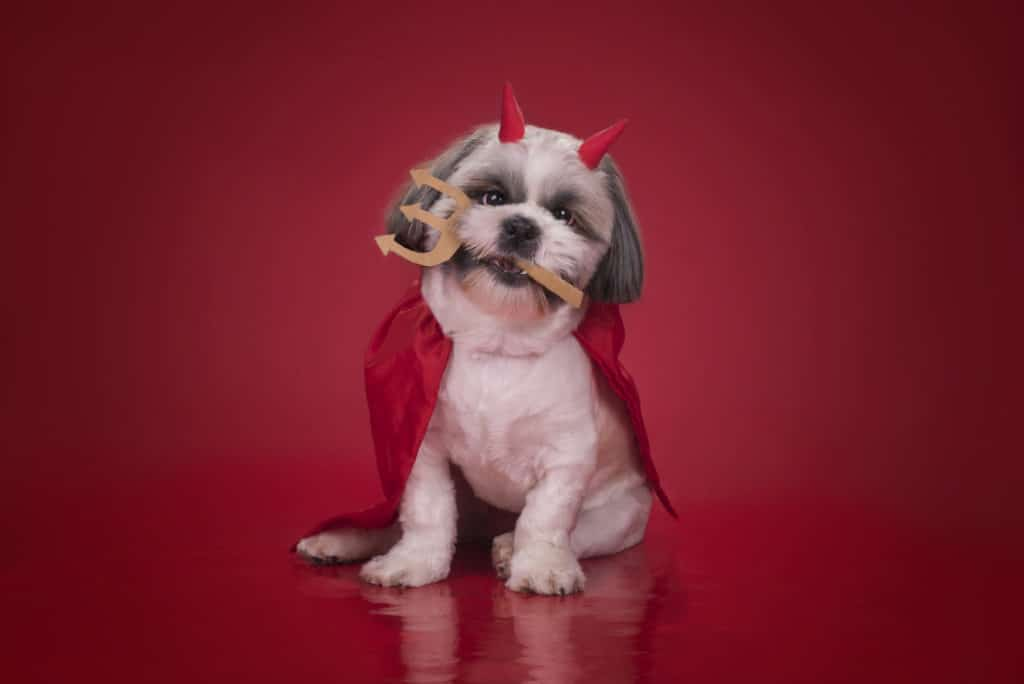
\includegraphics[max width=0.5\textwidth,
            max height=0.4\textheight]{Images/devil.jpg}
    }{}

    \vfill
  \end{frame}
}

\AtBeginSubsection[]{
  \begin{frame}
    \vfill
    \centering
    \begin{beamercolorbox}[sep=8pt,center,shadow=true,rounded=true]{title}
    \usebeamerfont{title}\insertsectionhead\par%
    \usebeamerfont{subtitle}\insertsubsectionhead\par%
    \end{beamercolorbox}
    \ifthenelse{\equal{\subsecname}{Answers}} {
        \begin{center}
        Unmute yourselves!
        \end{center}
    }
    \vfill
  \end{frame}
}
\begin{document}

\title{Welcome to Quarantine Trivia VI!\vspace{-0.5in}}
\date{}

\begin{frame}
\titlepage{}
\begin{center}

\includegraphics[max width=0.9\textwidth,
    max height=0.4\textheight]{Images/triviatitleframelogo.png}
\end{center}
\end{frame}

\begingroup{}
\begin{frame}[t]{Our Research Team}
Once again this week, our team of academic researchers has been searching through the
world's great libraries (online of course, to maintain social distancing) to assemble
challenging questions.\par%
\pause{}
\begin{center}
\begin{figure}[h]
\caption*{OUR RESEARCH TEAM}
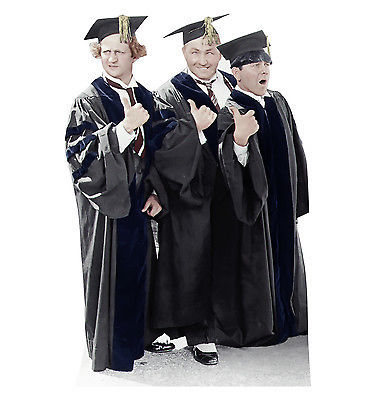
\includegraphics[max width=0.9\textwidth,
    max height=0.5\textheight]{{Images/threestooges}.jpg}
\end{figure}
\end{center}
\end{frame}
\endgroup{}

\begingroup{}
\begin{frame}[t]{Categories}
This week, they've come up with questions in the following categories:
\begin{enumerate}
\item Weather
\item Word Origins
\item Broadway Musical Names from Song Titles
\item Dog Breeds
\item Disney
\item National Parks
\item Rome
\item Books that had a Big Impact
\item Inventors and Inventions
\item California
\end{enumerate}
\end{frame}
\endgroup{}

\begingroup{}
\begin{frame}
\vfill{}
\begin{beamercolorbox}[sep=8pt,center,shadow=true,rounded=true]{title}
\usebeamerfont{title}Good luck everyone! And have fun!
\end{beamercolorbox}
\vfill{}
\end{frame}
\endgroup{}


\begin{frame}
\vfill
\centering
\begin{beamercolorbox}[sep=8pt,center,shadow=true,rounded=true]{title}
\usebeamerfont{title}Round 1\par%
\usebeamerfont{subtitle}Weather\par%
\end{beamercolorbox}
\begin{center}
Please mute yourselves!
\end{center}
\vfill
\end{frame}

\begin{frame}[t]{Weather, Question 1}

\begin{block}{Question}
The Inuit have approximately 50 different words for snow. Name any 15 of them.
\end{block}
\pause{}
\begin{block}{}
Sorry, couldn't resist! Now, on to the real game.
\end{block}
\end{frame}
\def\thisSectionName{Weather}
\section{Round 1}
\subsection*{Q1}
\begin{frame}[t]{Weather, Question 1}
% \vspace{0.5em}
\begin{block}{Question}
It's a myth that this effect leads to toilets flushing in the opposite direction in Australia, but the effect does cause hurricanes in the Northern and Southern hemispheres to rotate in opposite directions. What is the name of the effect?
\end{block}
\end{frame}
\subsection*{Q2}
\begin{frame}[t]{Weather, Question 2}
% \vspace{0.5em}
\begin{columns}[T,totalwidth=\linewidth]
\begin{column}{0.32\linewidth}
\begin{block}{Question}
What is the meteorological term for the thin, wispy clouds pictured here?
\end{block}
\end{column}
\begin{column}{0.65\linewidth}
\begin{center}
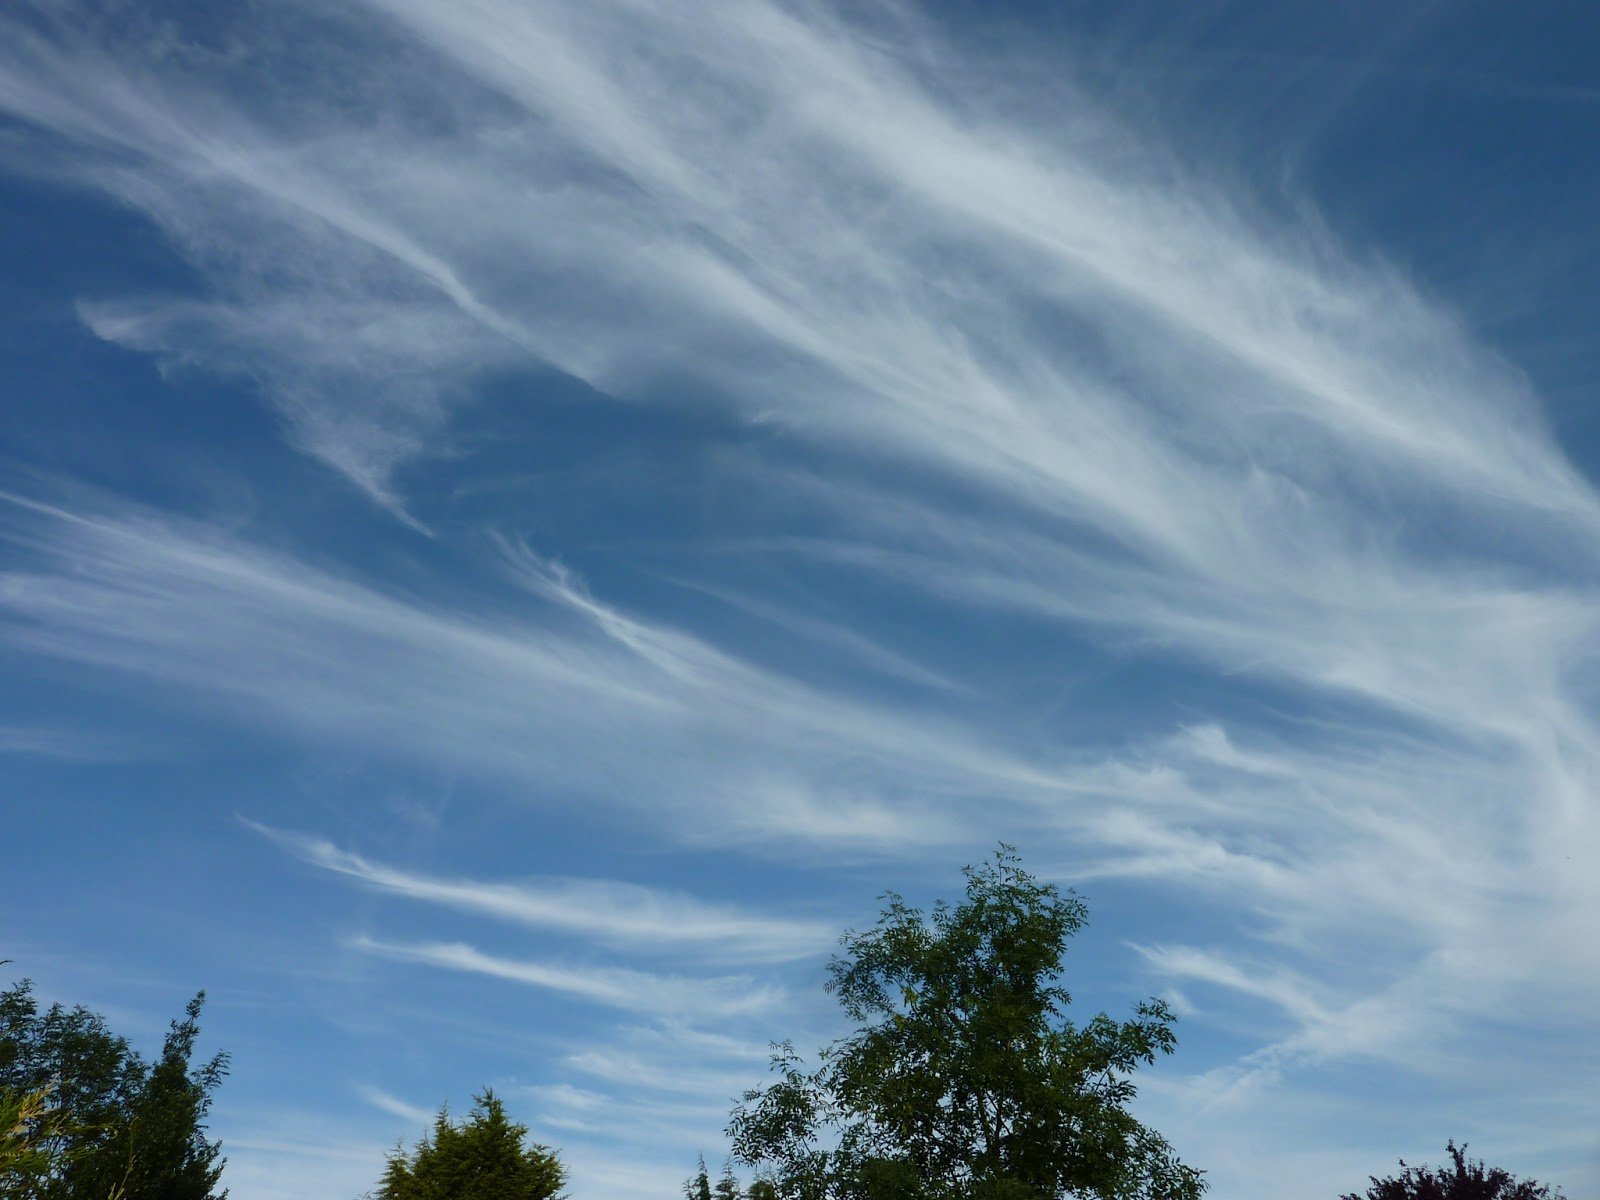
\includegraphics[max width=0.95\textwidth,max height=0.7\textheight]{{Images/cirrus}.jpg}
\end{center}
\end{column}
\end{columns}
\end{frame}
\subsection*{Q3}
\begin{frame}[t]{Weather, Question 3}
% \vspace{0.5em}
\begin{block}{Question}
Which two U.S. states are the only two that have never had a high temperature higher than 100\textdegree{}F\@?
\end{block}
\end{frame}
\subsection*{Q4}
\begin{frame}[t]{Weather, Question 4}
% \vspace{0.5em}
\begin{columns}[T,totalwidth=\linewidth]
\begin{column}{0.32\linewidth}
\begin{block}{Question}
The device pictured here measures wind speed and direction. What is it called?
\end{block}
\end{column}
\begin{column}{0.65\linewidth}
\begin{center}
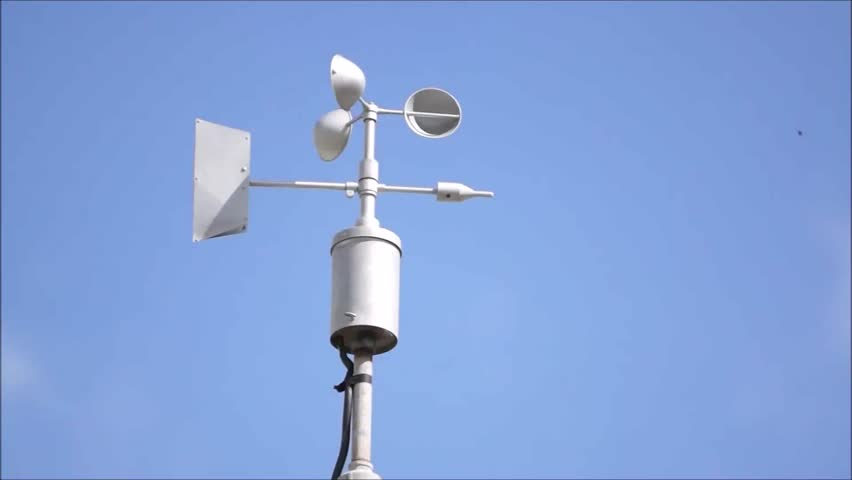
\includegraphics[max width=0.95\textwidth,max height=0.7\textheight]{{Images/anemometer}.jpg}
\end{center}
\end{column}
\end{columns}
\end{frame}
\subsection*{Q5}
\begin{frame}[t]{Weather, Question 5}
% \vspace{0.5em}
\begin{block}{Question}
The Tri-State Tornado of 1925 is both the deadliest tornado in U.S. history and the one with the longest path, which was approximately 220mi long. Name any one of the three states it hit.
\end{block}
\end{frame}
\subsection*{Q6}
\begin{frame}[t]{Weather, Question 6}
% \vspace{0.5em}
\begin{block}{Question}
What is the name of the scale that classifies hurricanes as category 1 to 5 based on their wind speed?
\end{block}
\end{frame}
\subsection*{Q7}
\begin{frame}[t]{Weather, Question 7}
% \vspace{0.5em}
\begin{block}{Question}
Spearfish, South Dakota holds the record for the most rapid temperature change ever recorded. To within 5 \textdegree{}F / 3 \textdegree{}C, how much did the air temperature there rise in the two-minute period over which this record-setting temperature change occurred?
\end{block}
\end{frame}
\subsection*{Q8}
\begin{frame}[t]{Weather, Question 8}
% \vspace{0.5em}
\begin{block}{Question}
On average, which U.S. state has the most tornadoes per year?
\end{block}
\end{frame}
\subsection*{Q9}
\begin{frame}[t]{Weather, Question 9}
% \vspace{0.5em}
\begin{columns}[T,totalwidth=\linewidth]
\begin{column}{0.32\linewidth}
\begin{block}{Question}
What is the name of the ice pictured here, which forms when water droplets in fog freeze to the surface of a solid object?
\end{block}
\end{column}
\begin{column}{0.65\linewidth}
\begin{center}
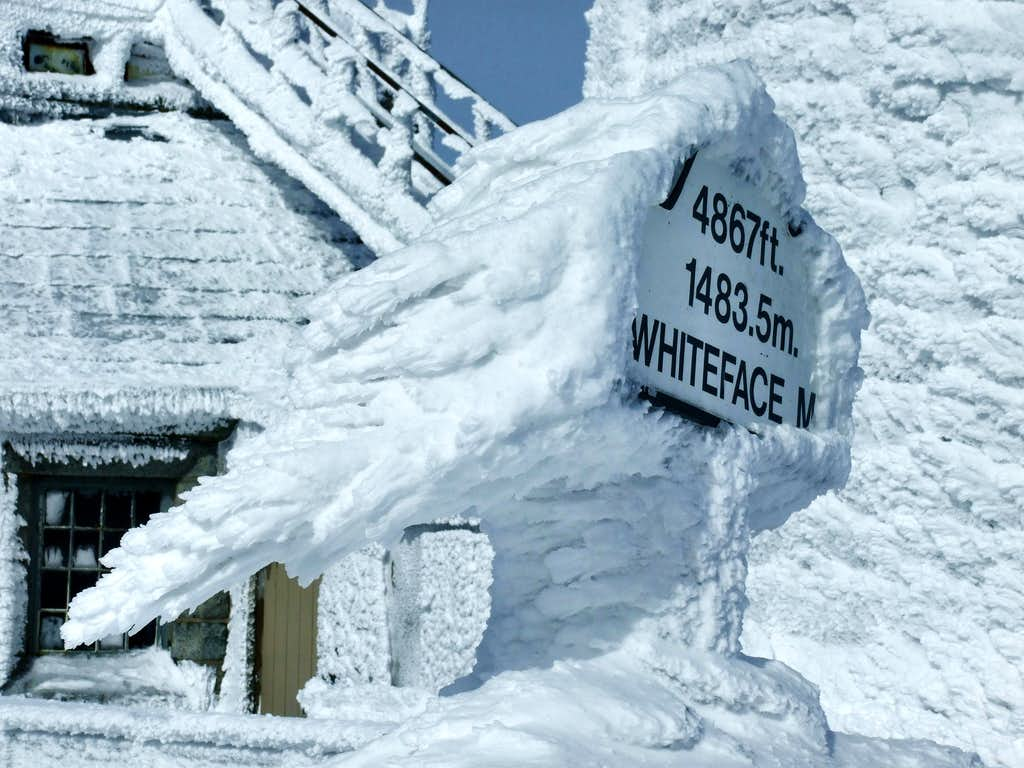
\includegraphics[max width=0.95\textwidth,max height=0.7\textheight]{{Images/rime}.jpg}
\end{center}
\end{column}
\end{columns}
\end{frame}
\subsection*{Q10}
\begin{frame}[t]{Weather, Question 10}
% \vspace{0.5em}
\begin{columns}[T,totalwidth=\linewidth]
\begin{column}{0.32\linewidth}
\begin{block}{Question}
What does this meteorological symbol indicate the approach of?
\end{block}
\end{column}
\begin{column}{0.65\linewidth}
\begin{center}
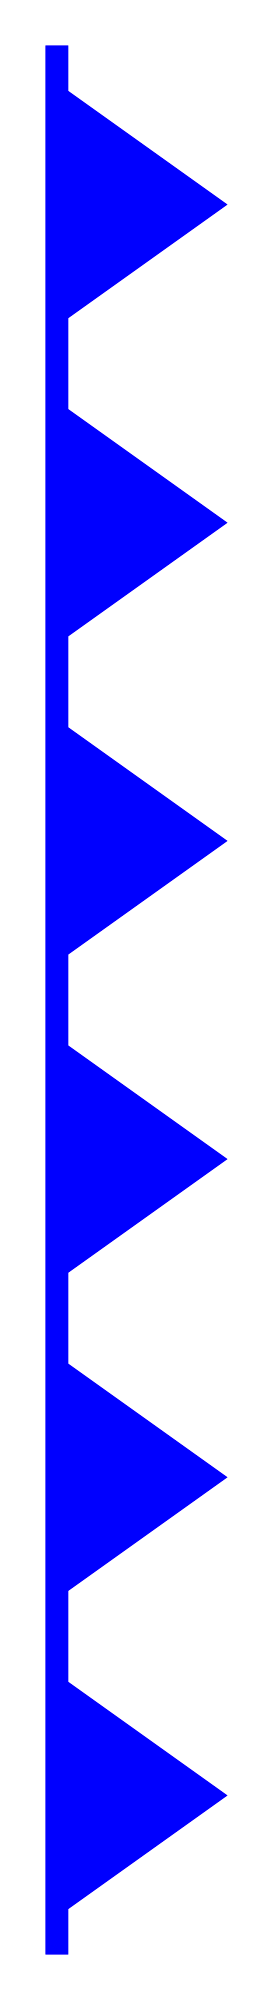
\includegraphics[max width=0.95\textwidth,max height=0.7\textheight]{{Images/coldfront}.png}
\end{center}
\end{column}
\end{columns}
\end{frame}
\subsection{Answers}
\begin{frame}[t]{Weather, Answer 1}
% \vspace{0.5em}
\begin{block}{Question}
It's a myth that this effect leads to toilets flushing in the opposite direction in Australia, but the effect does cause hurricanes in the Northern and Southern hemispheres to rotate in opposite directions. What is the name of the effect?
\end{block}

\visible<2->{
    \begin{columns}[T,totalwidth=\linewidth]
    \begin{column}{0.32\linewidth}
    \begin{block}{Answer}
    The Coriolis effect
    \end{block}
    \end{column}
    \begin{column}{0.65\linewidth}
    \begin{center}
    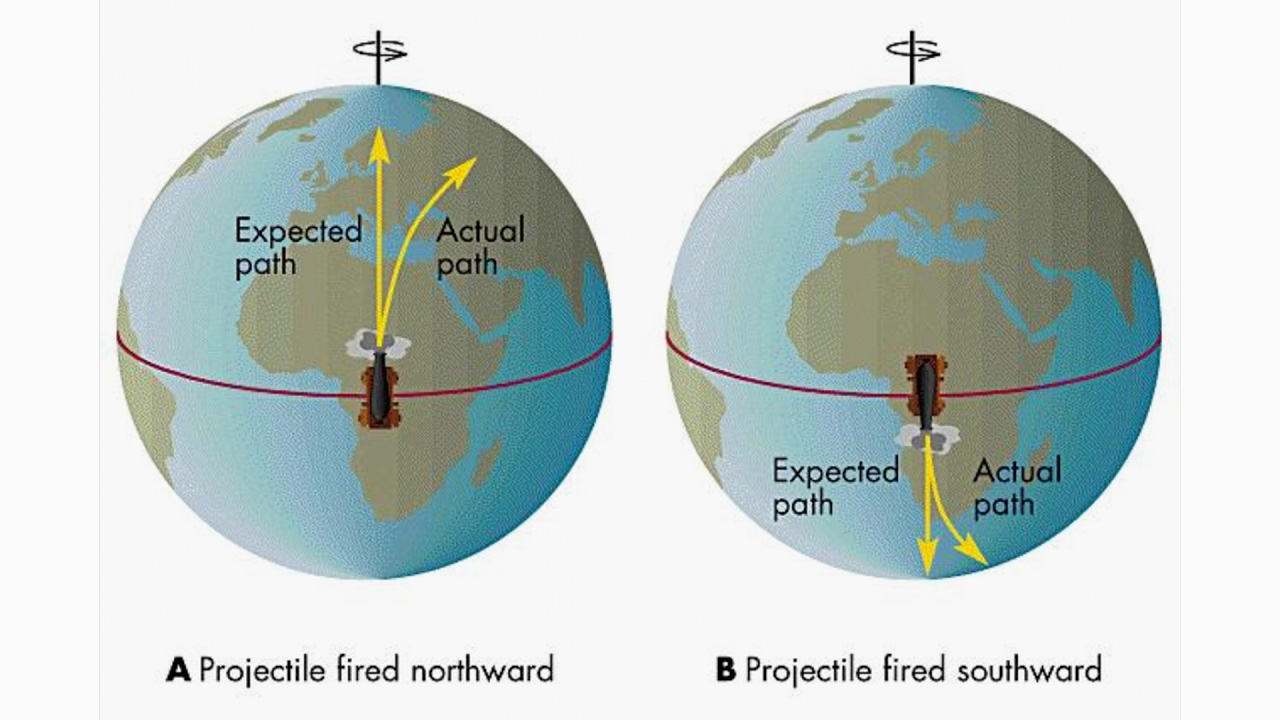
\includegraphics[max width=0.95\textwidth,
        max height=0.42000\textheight]{{Images/coriolis}.jpg}
    \end{center}
    \end{column}
    \end{columns}
}
\end{frame}
\begin{frame}[t]{Weather, Answer 2}
% \vspace{0.5em}
\begin{columns}[T,totalwidth=\linewidth]
\begin{column}{0.32\linewidth}
\begin{block}{Question}
What is the meteorological term for the thin, wispy clouds pictured here?
\end{block}
\visible<2->{
    \begin{block}{Answer}
    Cirrus clouds
    \end{block}
}
\end{column}
\begin{column}{0.65\linewidth}
\begin{center}
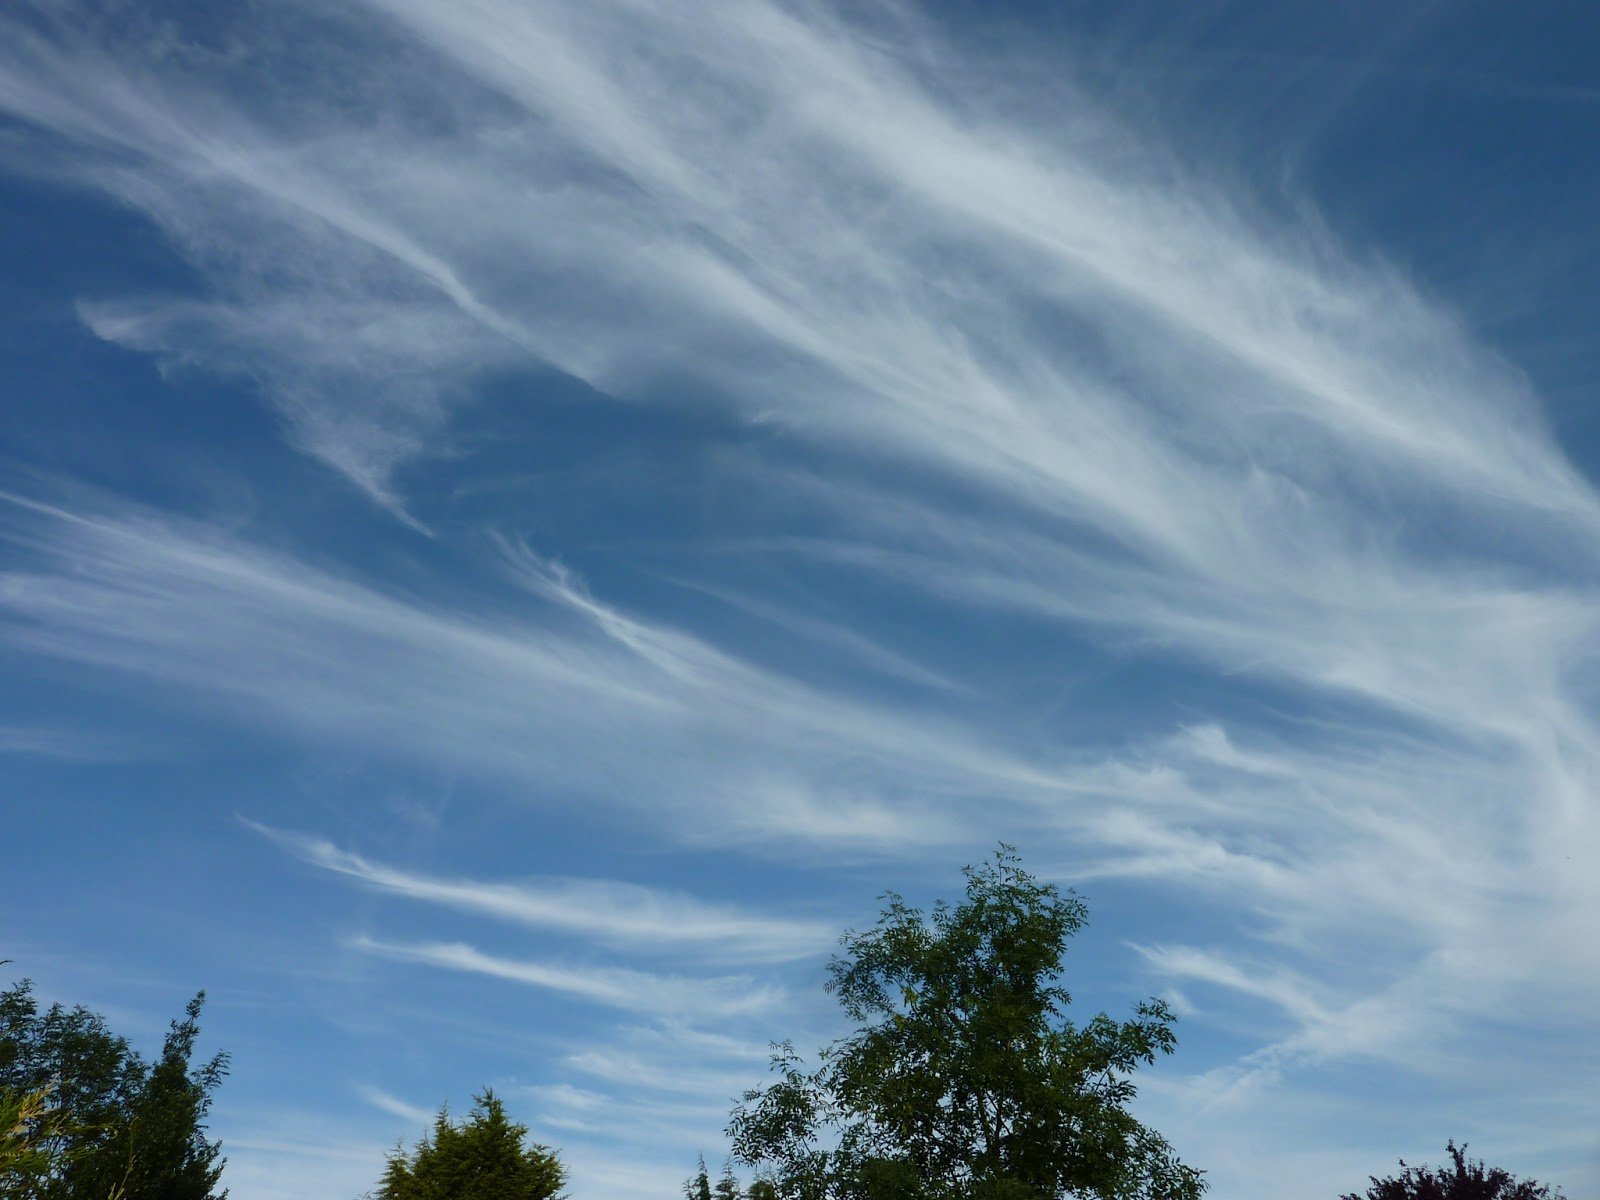
\includegraphics[max width=0.95\textwidth,max height=0.7\textheight]{{Images/cirrus}.jpg}
\end{center}
\end{column}
\end{columns}
\end{frame}
\begin{frame}[t]{Weather, Answer 3}
% \vspace{0.5em}
\begin{block}{Question}
Which two U.S. states are the only two that have never had a high temperature higher than 100\textdegree{}F\@?
\end{block}

\visible<2->{
    \begin{columns}[T,totalwidth=\linewidth]
    \begin{column}{0.32\linewidth}
    \begin{block}{Answer}
    Alaska and Hawaii
    \end{block}
    \end{column}
    \begin{column}{0.65\linewidth}
    \begin{center}
    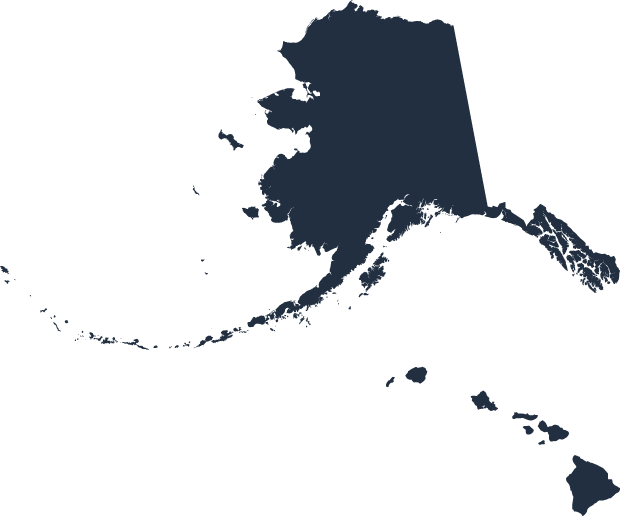
\includegraphics[max width=0.95\textwidth,
        max height=0.50000\textheight]{{Images/hightemp}.png}
    \end{center}
    \end{column}
    \end{columns}
}
\end{frame}
\begin{frame}[t]{Weather, Answer 4}
% \vspace{0.5em}
\begin{columns}[T,totalwidth=\linewidth]
\begin{column}{0.32\linewidth}
\begin{block}{Question}
The device pictured here measures wind speed and direction. What is it called?
\end{block}
\visible<2->{
    \begin{block}{Answer}
    Anemometer
    \end{block}
}
\end{column}
\begin{column}{0.65\linewidth}
\begin{center}
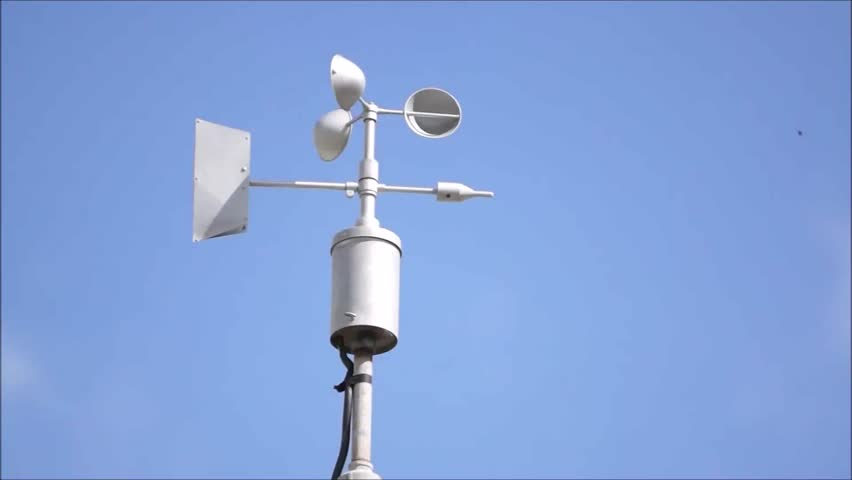
\includegraphics[max width=0.95\textwidth,max height=0.7\textheight]{{Images/anemometer}.jpg}
\end{center}
\end{column}
\end{columns}
\end{frame}
\begin{frame}[t]{Weather, Answer 5}
% \vspace{0.5em}
\begin{block}{Question}
The Tri-State Tornado of 1925 is both the deadliest tornado in U.S. history and the one with the longest path, which was approximately 220mi long. Name any one of the three states it hit.
\end{block}

\visible<2->{
    \begin{columns}[T,totalwidth=\linewidth]
    \begin{column}{0.32\linewidth}
    \begin{block}{Answer}
    Missouri, Illinois, Indiana
    \end{block}
    \end{column}
    \begin{column}{0.65\linewidth}
    \begin{center}
    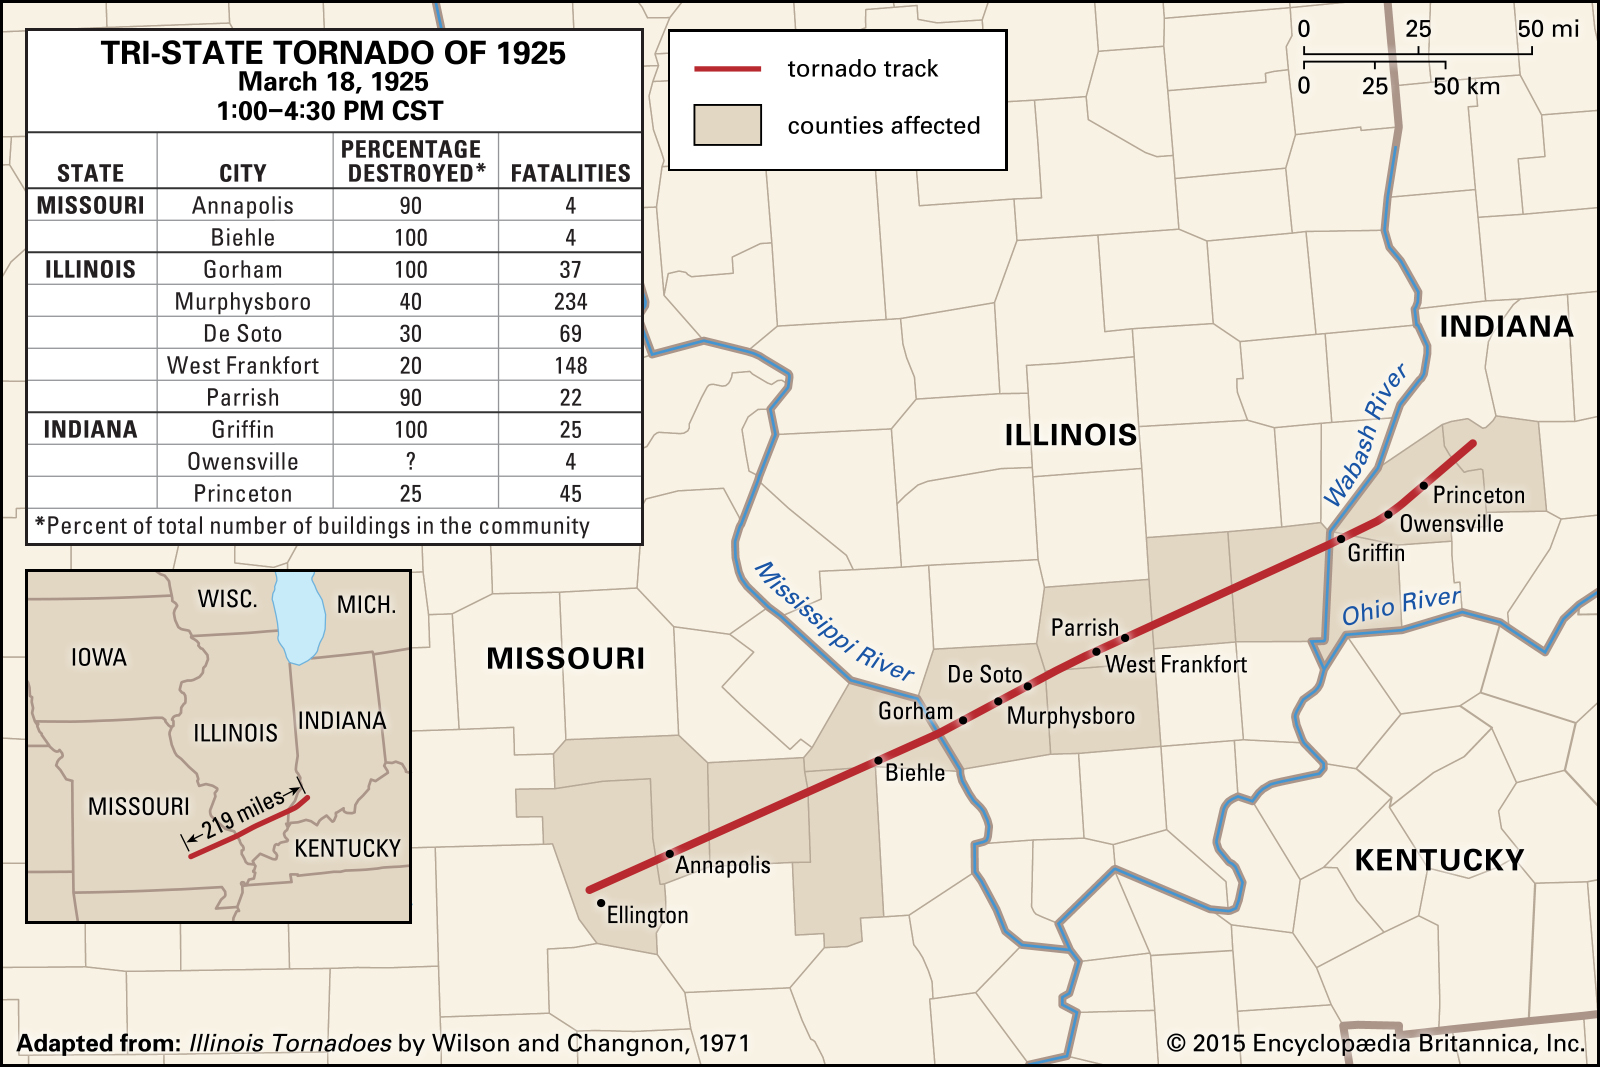
\includegraphics[max width=0.95\textwidth,
        max height=0.46000\textheight]{{Images/tristatetornado}.jpg}
    \end{center}
    \end{column}
    \end{columns}
}
\end{frame}
\begin{frame}[t]{Weather, Answer 6}
% \vspace{0.5em}
\begin{block}{Question}
What is the name of the scale that classifies hurricanes as category 1 to 5 based on their wind speed?
\end{block}

\visible<2->{
    \begin{columns}[T,totalwidth=\linewidth]
    \begin{column}{0.32\linewidth}
    \begin{block}{Answer}
    The Saffir-Simpson scale
    \end{block}
    \end{column}
    \begin{column}{0.65\linewidth}
    \begin{center}
    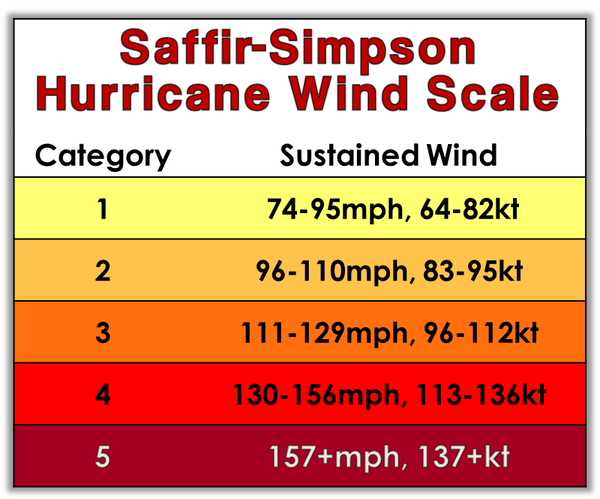
\includegraphics[max width=0.95\textwidth,
        max height=0.50000\textheight]{{Images/saffirsimpson}.png}
    \end{center}
    \end{column}
    \end{columns}
}
\end{frame}
\begin{frame}[t]{Weather, Answer 7}
% \vspace{0.5em}
\begin{block}{Question}
Spearfish, South Dakota holds the record for the most rapid temperature change ever recorded. To within 5 \textdegree{}F / 3 \textdegree{}C, how much did the air temperature there rise in the two-minute period over which this record-setting temperature change occurred?
\end{block}

\visible<2->{
    \begin{columns}[T,totalwidth=\linewidth]
    \begin{column}{0.32\linewidth}
    \begin{block}{Answer}
    49 \textdegree{}F / 27 \textdegree{}C (44--54 \textdegree{}F / 24--30 \textdegree{}C will be accepted)
    \end{block}
    \end{column}
    \begin{column}{0.65\linewidth}
    \begin{center}
    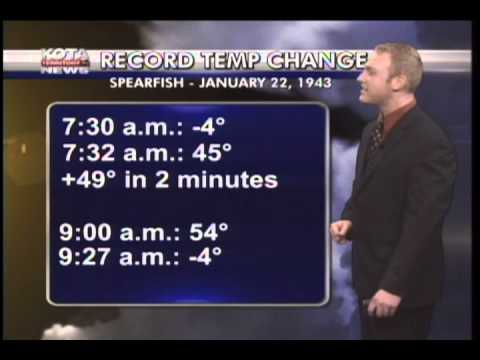
\includegraphics[max width=0.95\textwidth,
        max height=0.38000\textheight]{{Images/spearfish}.jpg}
    \end{center}
    \end{column}
    \end{columns}
}
\end{frame}
\begin{frame}[t]{Weather, Answer 8}
% \vspace{0.5em}
\begin{block}{Question}
On average, which U.S. state has the most tornadoes per year?
\end{block}
\visible<2->{
    \begin{block}{Answer}
    Texas (approx.\ 135 annually)
    \end{block}
}
\end{frame}
\begin{frame}[t]{Weather, Answer 9}
% \vspace{0.5em}
\begin{columns}[T,totalwidth=\linewidth]
\begin{column}{0.32\linewidth}
\begin{block}{Question}
What is the name of the ice pictured here, which forms when water droplets in fog freeze to the surface of a solid object?
\end{block}
\visible<2->{
    \begin{block}{Answer}
    Rime
    \end{block}
}
\end{column}
\begin{column}{0.65\linewidth}
\begin{center}
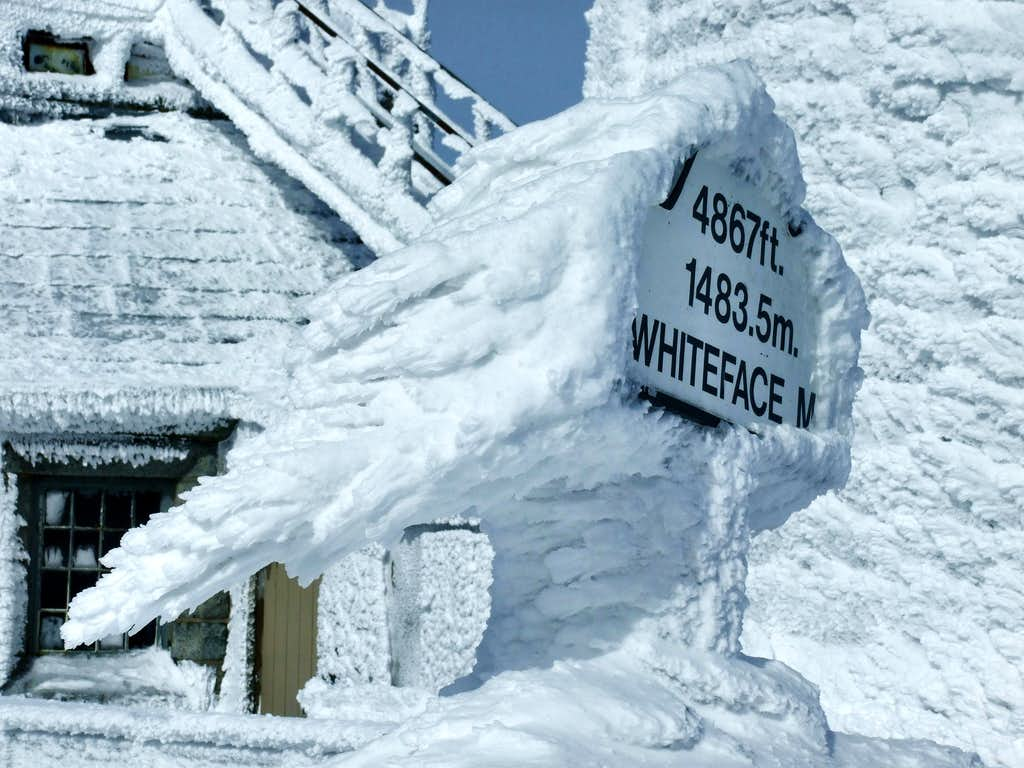
\includegraphics[max width=0.95\textwidth,max height=0.7\textheight]{{Images/rime}.jpg}
\end{center}
\end{column}
\end{columns}
\end{frame}
\begin{frame}[t]{Weather, Answer 10}
% \vspace{0.5em}
\begin{columns}[T,totalwidth=\linewidth]
\begin{column}{0.32\linewidth}
\begin{block}{Question}
What does this meteorological symbol indicate the approach of?
\end{block}
\visible<2->{
    \begin{block}{Answer}
    A cold front
    \end{block}
}
\end{column}
\begin{column}{0.65\linewidth}
\begin{center}
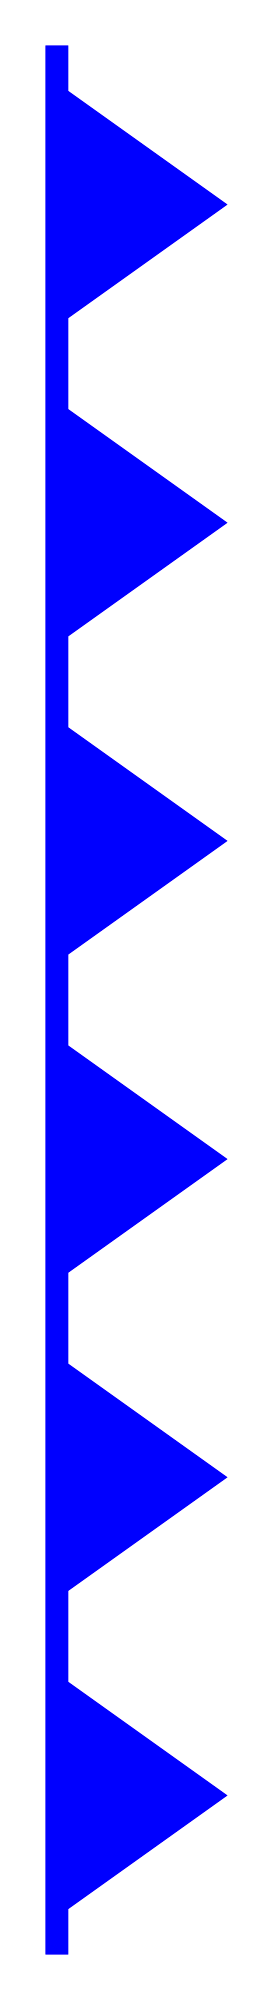
\includegraphics[max width=0.95\textwidth,max height=0.7\textheight]{{Images/coldfront}.png}
\end{center}
\end{column}
\end{columns}
\end{frame}
\def\thisSectionName{Word Origins}
\section{Round 2}
\subsection*{Q1}
\begin{frame}[t]{Word Origins, Question 1}
% \vspace{0.5em}
\begin{block}{Question}
The name of which contraption is a combination of the Greek words for ``spiral'' and ``wing''?
\end{block}
\end{frame}
\subsection*{Q2}
\begin{frame}[t]{Word Origins, Question 2}
% \vspace{0.5em}
\begin{block}{Question}
Which word that is synonymous with ``calamity'' comes from the Greek for, literally, ``ill-starred'', stemming from the ancient superstition that the stars determined one's fate?
\end{block}
\end{frame}
\subsection*{Q3}
\begin{frame}[t]{Word Origins, Question 3}
% \vspace{0.5em}
\begin{block}{Question}
The word ``first'' is derived from the superlative of which adjective that has a related meaning?
\end{block}
\end{frame}
\subsection*{Q4}
\begin{frame}[t]{Word Origins, Question 4}
% \vspace{0.5em}
\begin{columns}[T,totalwidth=\linewidth]
\begin{column}{0.32\linewidth}
\begin{block}{Question}
The name of the Civil War general pictured here is the origin of the word for a particular style of facial hair. What is the general's name?
\end{block}
\end{column}
\begin{column}{0.65\linewidth}
\begin{center}
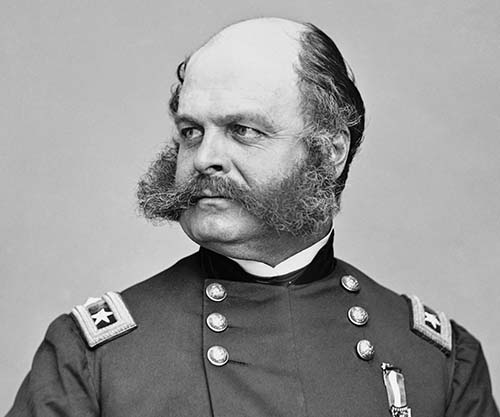
\includegraphics[max width=0.95\textwidth,max height=0.7\textheight]{{Images/burnsides}.jpg}
\end{center}
\end{column}
\end{columns}
\end{frame}
\subsection*{Q5}
\begin{frame}[t]{Word Origins, Question 5}
% \vspace{0.5em}
\begin{block}{Question}
Which English word is derived from an ancient Greek word that meant ``foreigner'' and that was onomatopoetic in that it resembled the sound of foreign or unintelligible speech?
\end{block}
\end{frame}
\subsection*{Q6}
\begin{frame}[t]{Word Origins, Question 6}
% \vspace{0.5em}
\begin{block}{Question}
This name of a region of the Earth comes from the Greek for ``bear'' (the animal), as it was thought to lie beneath Ursa Major, the bear constellation.
\end{block}
\end{frame}
\subsection*{Q7}
\begin{frame}[t]{Word Origins, Question 7}
% \vspace{0.5em}
\begin{block}{Question}
Which animal's name is Afrikaans Dutch for ``ground-pig''?
\end{block}
\end{frame}
\subsection*{Q8}
\begin{frame}[t]{Word Origins, Question 8}
% \vspace{0.5em}
\begin{block}{Question}
The word for this kind of book was taken directly from a Latin word that originally meant ``treasury'' but whose meaning expanded to mean any kind of repository.
\end{block}
\end{frame}
\subsection*{Q9}
\begin{frame}[t]{Word Origins, Question 9}
% \vspace{0.5em}
\begin{block}{Question}
What current English word is an amalgam of the Ancient Greek words for ``crappy'' and ``sound''?
\end{block}
\end{frame}
\subsection*{Q10}
\begin{frame}[t]{Word Origins, Question 10}
% \vspace{0.5em}
\begin{block}{Question}
Which word's origin is the Medieval Latin collective noun for the first three of the seven liberal arts (grammar, rhetoric, and logic), which itself ultimately comes from the Latin for ``place where three roads meet''?
\end{block}
\end{frame}
\subsection{Answers}
\begin{frame}[t]{Word Origins, Answer 1}
% \vspace{0.5em}
\begin{block}{Question}
The name of which contraption is a combination of the Greek words for ``spiral'' and ``wing''?
\end{block}

\visible<2->{
    \begin{columns}[T,totalwidth=\linewidth]
    \begin{column}{0.32\linewidth}
    \begin{block}{Answer}
    Helicopter (helico + pter)
    \end{block}
    \end{column}
    \begin{column}{0.65\linewidth}
    \begin{center}
    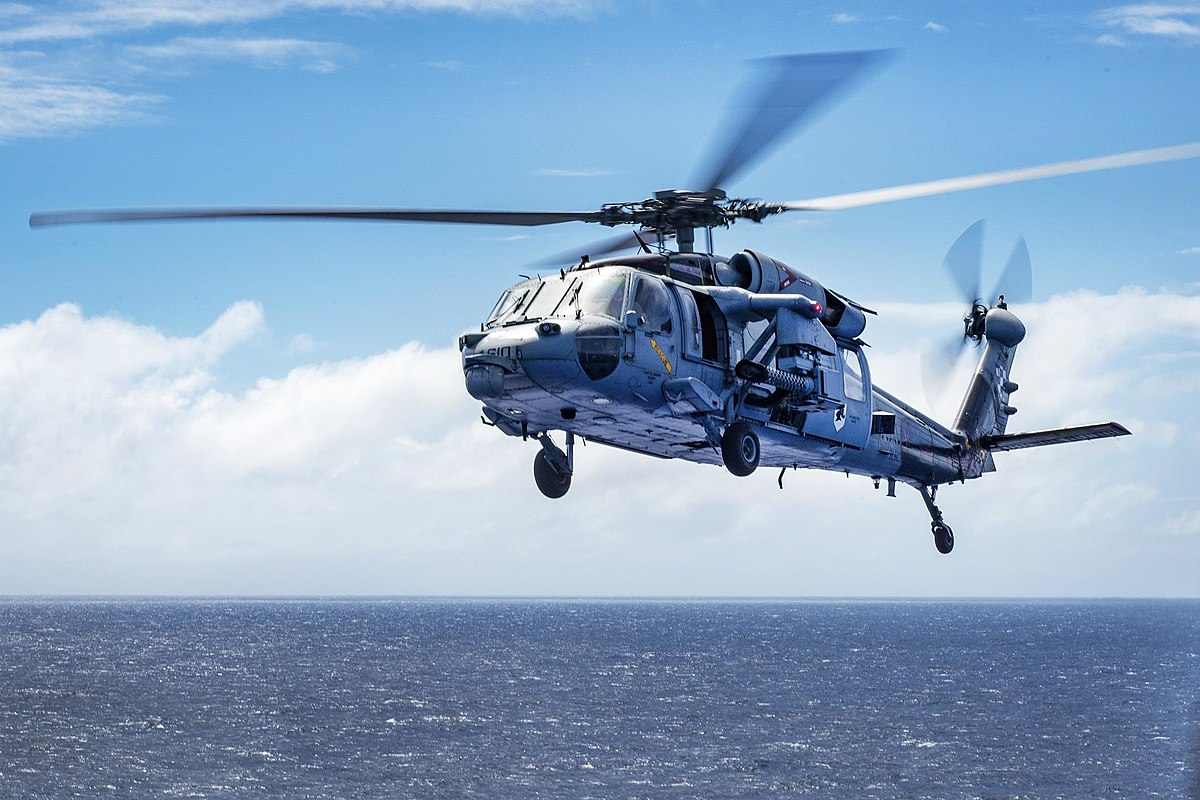
\includegraphics[max width=0.95\textwidth,
        max height=0.54000\textheight]{{Images/helicopter}.jpeg}
    \end{center}
    \end{column}
    \end{columns}
}
\end{frame}
\begin{frame}[t]{Word Origins, Answer 2}
% \vspace{0.5em}
\begin{block}{Question}
Which word that is synonymous with ``calamity'' comes from the Greek for, literally, ``ill-starred'', stemming from the ancient superstition that the stars determined one's fate?
\end{block}
\visible<2->{
    \begin{block}{Answer}
    Disaster
    \end{block}
}
\end{frame}
\begin{frame}[t]{Word Origins, Answer 3}
% \vspace{0.5em}
\begin{block}{Question}
The word ``first'' is derived from the superlative of which adjective that has a related meaning?
\end{block}
\visible<2->{
    \begin{block}{Answer}
    Fore
    \end{block}
}
\end{frame}
\begin{frame}[t]{Word Origins, Answer 4}
% \vspace{0.5em}
\begin{columns}[T,totalwidth=\linewidth]
\begin{column}{0.32\linewidth}
\begin{block}{Question}
The name of the Civil War general pictured here is the origin of the word for a particular style of facial hair. What is the general's name?
\end{block}
\visible<2->{
    \begin{block}{Answer}
    General Burnsides
    \end{block}
}
\end{column}
\begin{column}{0.65\linewidth}
\begin{center}
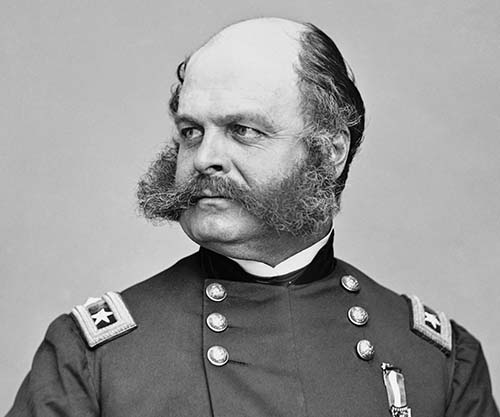
\includegraphics[max width=0.95\textwidth,max height=0.7\textheight]{{Images/burnsides}.jpg}
\end{center}
\end{column}
\end{columns}
\end{frame}
\begin{frame}[t]{Word Origins, Answer 5}
% \vspace{0.5em}
\begin{block}{Question}
Which English word is derived from an ancient Greek word that meant ``foreigner'' and that was onomatopoetic in that it resembled the sound of foreign or unintelligible speech?
\end{block}

\visible<2->{
    \begin{columns}[T,totalwidth=\linewidth]
    \begin{column}{0.32\linewidth}
    \begin{block}{Answer}
    Barbarian or barbaric
    \end{block}
    \end{column}
    \begin{column}{0.65\linewidth}
    \begin{center}
    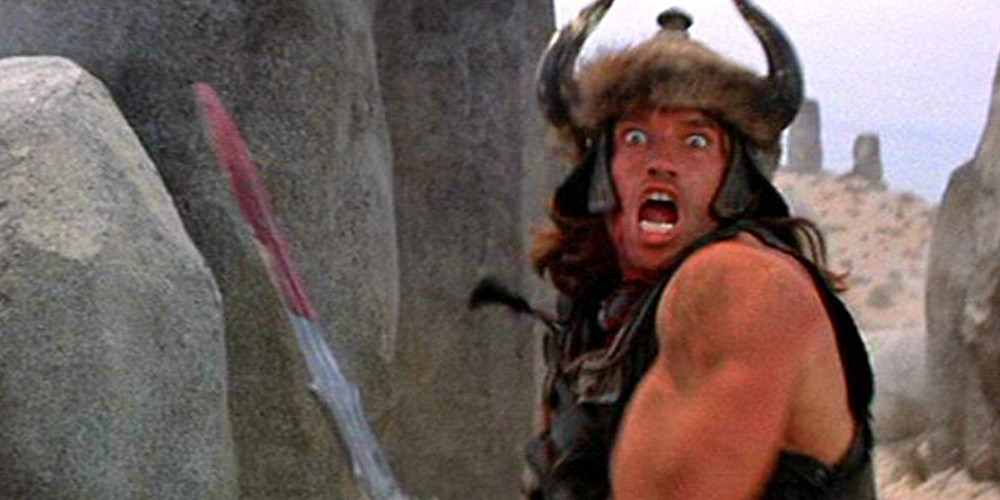
\includegraphics[max width=0.95\textwidth,
        max height=0.46000\textheight]{{Images/barbarian}.jpg}
    \end{center}
    \end{column}
    \end{columns}
}
\end{frame}
\begin{frame}[t]{Word Origins, Answer 6}
% \vspace{0.5em}
\begin{block}{Question}
This name of a region of the Earth comes from the Greek for ``bear'' (the animal), as it was thought to lie beneath Ursa Major, the bear constellation.
\end{block}

\visible<2->{
    \begin{columns}[T,totalwidth=\linewidth]
    \begin{column}{0.32\linewidth}
    \begin{block}{Answer}
    The Arctic (from Greek \emph{arktos})
    \end{block}
    \end{column}
    \begin{column}{0.65\linewidth}
    \begin{center}
    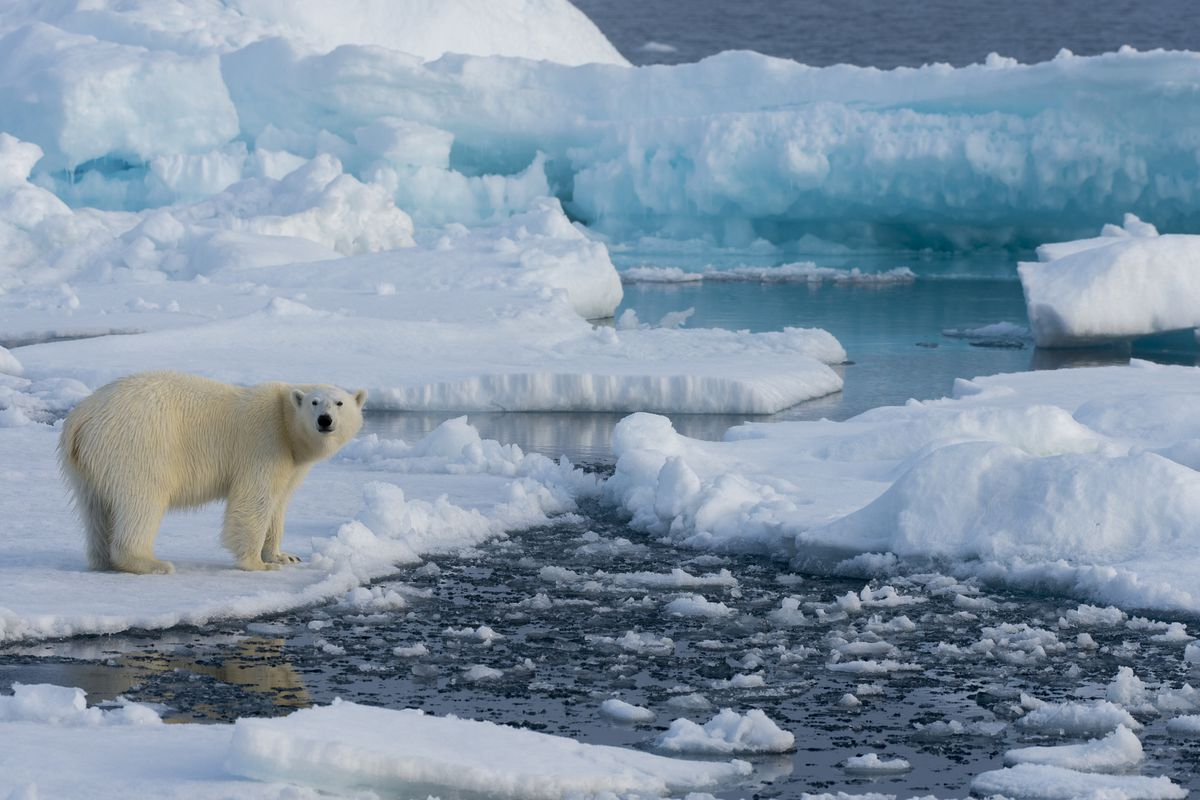
\includegraphics[max width=0.95\textwidth,
        max height=0.46000\textheight]{{Images/arctic}.jpg}
    \end{center}
    \end{column}
    \end{columns}
}
\end{frame}
\begin{frame}[t]{Word Origins, Answer 7}
% \vspace{0.5em}
\begin{block}{Question}
Which animal's name is Afrikaans Dutch for ``ground-pig''?
\end{block}

\visible<2->{
    \begin{columns}[T,totalwidth=\linewidth]
    \begin{column}{0.32\linewidth}
    \begin{block}{Answer}
    Aardvark
    \end{block}
    \end{column}
    \begin{column}{0.65\linewidth}
    \begin{center}
    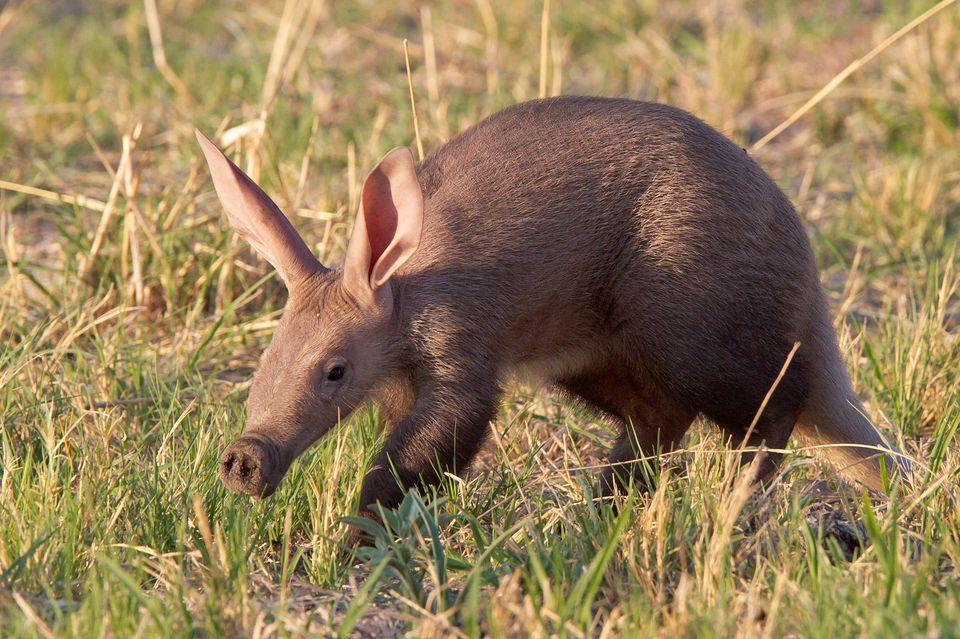
\includegraphics[max width=0.95\textwidth,
        max height=0.54000\textheight]{{Images/aardvark}.jpg}
    \end{center}
    \end{column}
    \end{columns}
}
\end{frame}
\begin{frame}[t]{Word Origins, Answer 8}
% \vspace{0.5em}
\begin{block}{Question}
The word for this kind of book was taken directly from a Latin word that originally meant ``treasury'' but whose meaning expanded to mean any kind of repository.
\end{block}

\visible<2->{
    \begin{columns}[T,totalwidth=\linewidth]
    \begin{column}{0.32\linewidth}
    \begin{block}{Answer}
    Thesaurus
    \end{block}
    \end{column}
    \begin{column}{0.65\linewidth}
    \begin{center}
    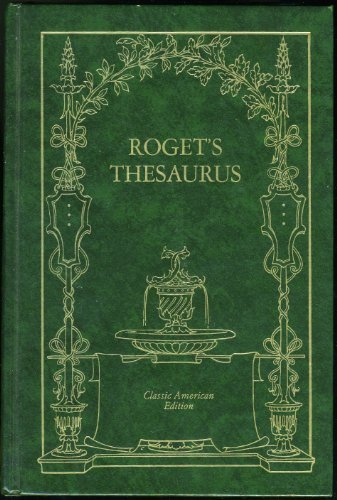
\includegraphics[max width=0.95\textwidth,
        max height=0.46000\textheight]{{Images/roget}.jpg}
    \end{center}
    \end{column}
    \end{columns}
}
\end{frame}
\begin{frame}[t]{Word Origins, Answer 9}
% \vspace{0.5em}
\begin{block}{Question}
What current English word is an amalgam of the Ancient Greek words for ``crappy'' and ``sound''?
\end{block}
\visible<2->{
    \begin{block}{Answer}
    Cacophony
    \end{block}
}
\end{frame}
\begin{frame}[t]{Word Origins, Answer 10}
% \vspace{0.5em}
\begin{block}{Question}
Which word's origin is the Medieval Latin collective noun for the first three of the seven liberal arts (grammar, rhetoric, and logic), which itself ultimately comes from the Latin for ``place where three roads meet''?
\end{block}

\visible<2->{
    \begin{columns}[T,totalwidth=\linewidth]
    \begin{column}{0.32\linewidth}
    \begin{block}{Answer}
    Trivia!
    \end{block}
    \end{column}
    \begin{column}{0.65\linewidth}
    \begin{center}
    
\includegraphics[max width=0.95\textwidth,
        max height=0.42000\textheight]{{Images/triviatitleframelogo}.png}
    \end{center}
    \end{column}
    \end{columns}
}
\end{frame}
\def\thisSectionName{Broadway Musical Names from Song Titles}
\section{Round 3}
\subsection*{Q1}
\begin{frame}[t]{Broadway Musical Names from Song Titles, Question 1}
% \vspace{0.5em}
\begin{block}{Question}
Just you Wait
\end{block}
\end{frame}
\subsection*{Q2}
\begin{frame}[t]{Broadway Musical Names from Song Titles, Question 2}
% \vspace{0.5em}
\begin{block}{Question}
No One is Alone
\end{block}
\end{frame}
\subsection*{Q3}
\begin{frame}[t]{Broadway Musical Names from Song Titles, Question 3}
% \vspace{0.5em}
\begin{block}{Question}
There's No Business Like Show Business
\end{block}
\end{frame}
\subsection*{Q4}
\begin{frame}[t]{Broadway Musical Names from Song Titles, Question 4}
% \vspace{0.5em}
\begin{block}{Question}
Bill
\end{block}
\end{frame}
\subsection*{Q5}
\begin{frame}[t]{Broadway Musical Names from Song Titles, Question 5}
% \vspace{0.5em}
\begin{block}{Question}
If I Were a Bell
\end{block}
\end{frame}
\subsection*{Q6}
\begin{frame}[t]{Broadway Musical Names from Song Titles, Question 6}
% \vspace{0.5em}
\begin{block}{Question}
What I Did for Love
\end{block}
\end{frame}
\subsection*{Q7}
\begin{frame}[t]{Broadway Musical Names from Song Titles, Question 7}
% \vspace{0.5em}
\begin{block}{Question}
Out Tonight
\end{block}
\end{frame}
\subsection*{Q8}
\begin{frame}[t]{Broadway Musical Names from Song Titles, Question 8}
% \vspace{0.5em}
\begin{block}{Question}
The King of Broadway
\end{block}
\end{frame}
\subsection*{Q9}
\begin{frame}[t]{Broadway Musical Names from Song Titles, Question 9}
% \vspace{0.5em}
\begin{block}{Question}
Cool
\end{block}
\end{frame}
\subsection*{Q10}
\begin{frame}[t]{Broadway Musical Names from Song Titles, Question 10}
% \vspace{0.5em}
\begin{block}{Question}
It Might as Well be Spring
\end{block}
\end{frame}
\subsection{Answers}
\begin{frame}[t]{Broadway Musical Names from Song Titles, Answer 1}
% \vspace{0.5em}
\begin{block}{Question}
Just you Wait
\end{block}

\visible<2->{
    \begin{columns}[T,totalwidth=\linewidth]
    \begin{column}{0.32\linewidth}
    \begin{block}{Answer}
    \emph{My Fair Lady}
    \end{block}
    \end{column}
    \begin{column}{0.65\linewidth}
    \begin{center}
    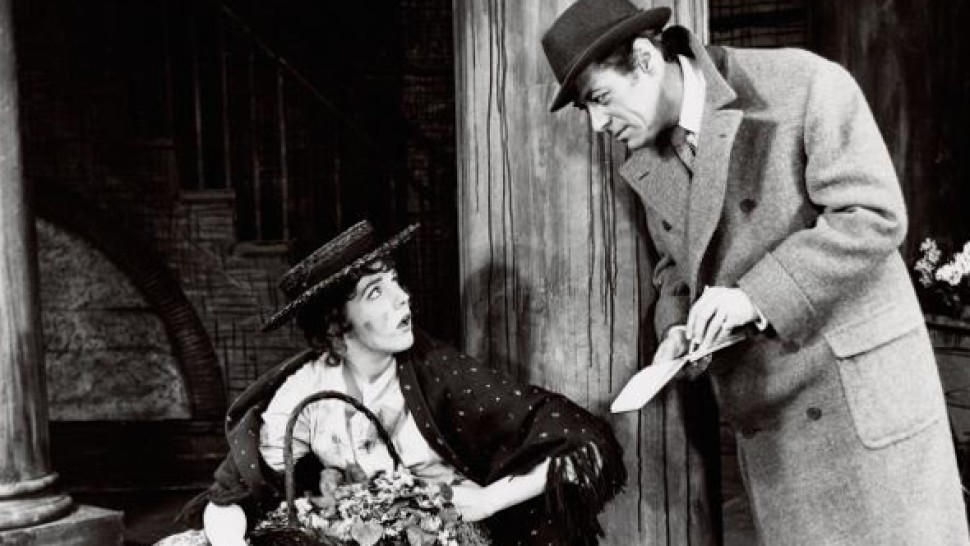
\includegraphics[max width=0.95\textwidth,
        max height=0.58000\textheight]{{Images/myfairlady}.jpeg}
    \end{center}
    \end{column}
    \end{columns}
}
\end{frame}
\begin{frame}[t]{Broadway Musical Names from Song Titles, Answer 2}
% \vspace{0.5em}
\begin{block}{Question}
No One is Alone
\end{block}

\visible<2->{
    \begin{columns}[T,totalwidth=\linewidth]
    \begin{column}{0.32\linewidth}
    \begin{block}{Answer}
    \emph{Into the Woods}
    \end{block}
    \end{column}
    \begin{column}{0.65\linewidth}
    \begin{center}
    
\includegraphics[max width=0.95\textwidth,
        max height=0.58000\textheight]{{Images/intowoods}.jpg}
    \end{center}
    \end{column}
    \end{columns}
}
\end{frame}
\begin{frame}[t]{Broadway Musical Names from Song Titles, Answer 3}
% \vspace{0.5em}
\begin{block}{Question}
There's No Business Like Show Business
\end{block}

\visible<2->{
    \begin{columns}[T,totalwidth=\linewidth]
    \begin{column}{0.32\linewidth}
    \begin{block}{Answer}
    \emph{Annie Get your Gun}
    \end{block}
    \end{column}
    \begin{column}{0.65\linewidth}
    \begin{center}
    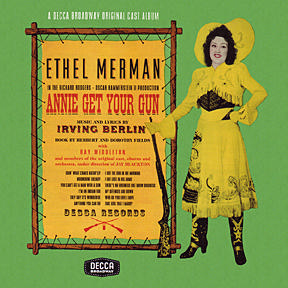
\includegraphics[max width=0.95\textwidth,
        max height=0.58000\textheight]{{Images/anniegun}.jpg}
    \end{center}
    \end{column}
    \end{columns}
}
\end{frame}
\begin{frame}[t]{Broadway Musical Names from Song Titles, Answer 4}
% \vspace{0.5em}
\begin{block}{Question}
Bill
\end{block}

\visible<2->{
    \begin{columns}[T,totalwidth=\linewidth]
    \begin{column}{0.32\linewidth}
    \begin{block}{Answer}
    \emph{Showboat}
    \end{block}
    \end{column}
    \begin{column}{0.65\linewidth}
    \begin{center}
    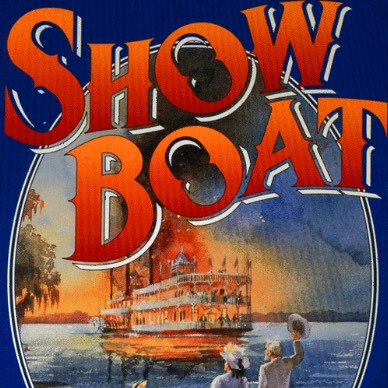
\includegraphics[max width=0.95\textwidth,
        max height=0.58000\textheight]{{Images/showboat}.jpg}
    \end{center}
    \end{column}
    \end{columns}
}
\end{frame}
\begin{frame}[t]{Broadway Musical Names from Song Titles, Answer 5}
% \vspace{0.5em}
\begin{block}{Question}
If I Were a Bell
\end{block}

\visible<2->{
    \begin{columns}[T,totalwidth=\linewidth]
    \begin{column}{0.32\linewidth}
    \begin{block}{Answer}
    \emph{Guys and Dolls}
    \end{block}
    \end{column}
    \begin{column}{0.65\linewidth}
    \begin{center}
    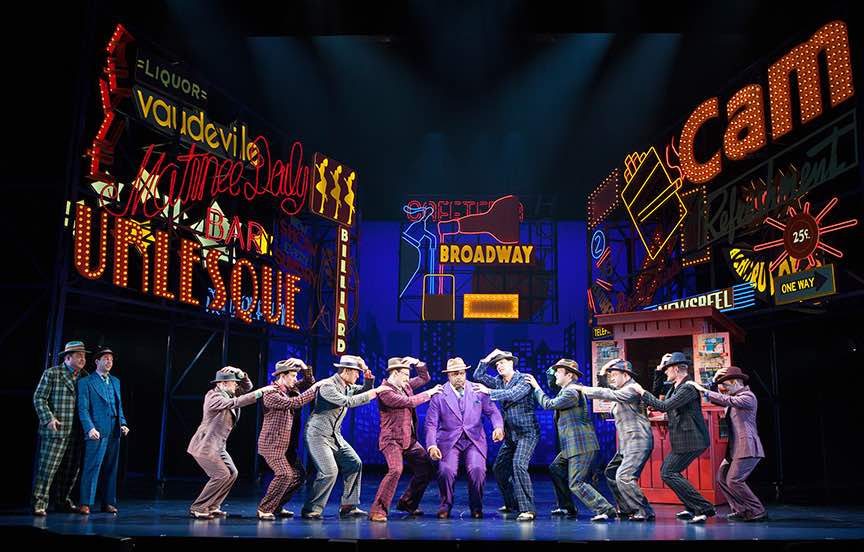
\includegraphics[max width=0.95\textwidth,
        max height=0.58000\textheight]{{Images/guysanddolls}.jpg}
    \end{center}
    \end{column}
    \end{columns}
}
\end{frame}
\begin{frame}[t]{Broadway Musical Names from Song Titles, Answer 6}
% \vspace{0.5em}
\begin{block}{Question}
What I Did for Love
\end{block}

\visible<2->{
    \begin{columns}[T,totalwidth=\linewidth]
    \begin{column}{0.32\linewidth}
    \begin{block}{Answer}
    \emph{A Chorus Line}
    \end{block}
    \end{column}
    \begin{column}{0.65\linewidth}
    \begin{center}
    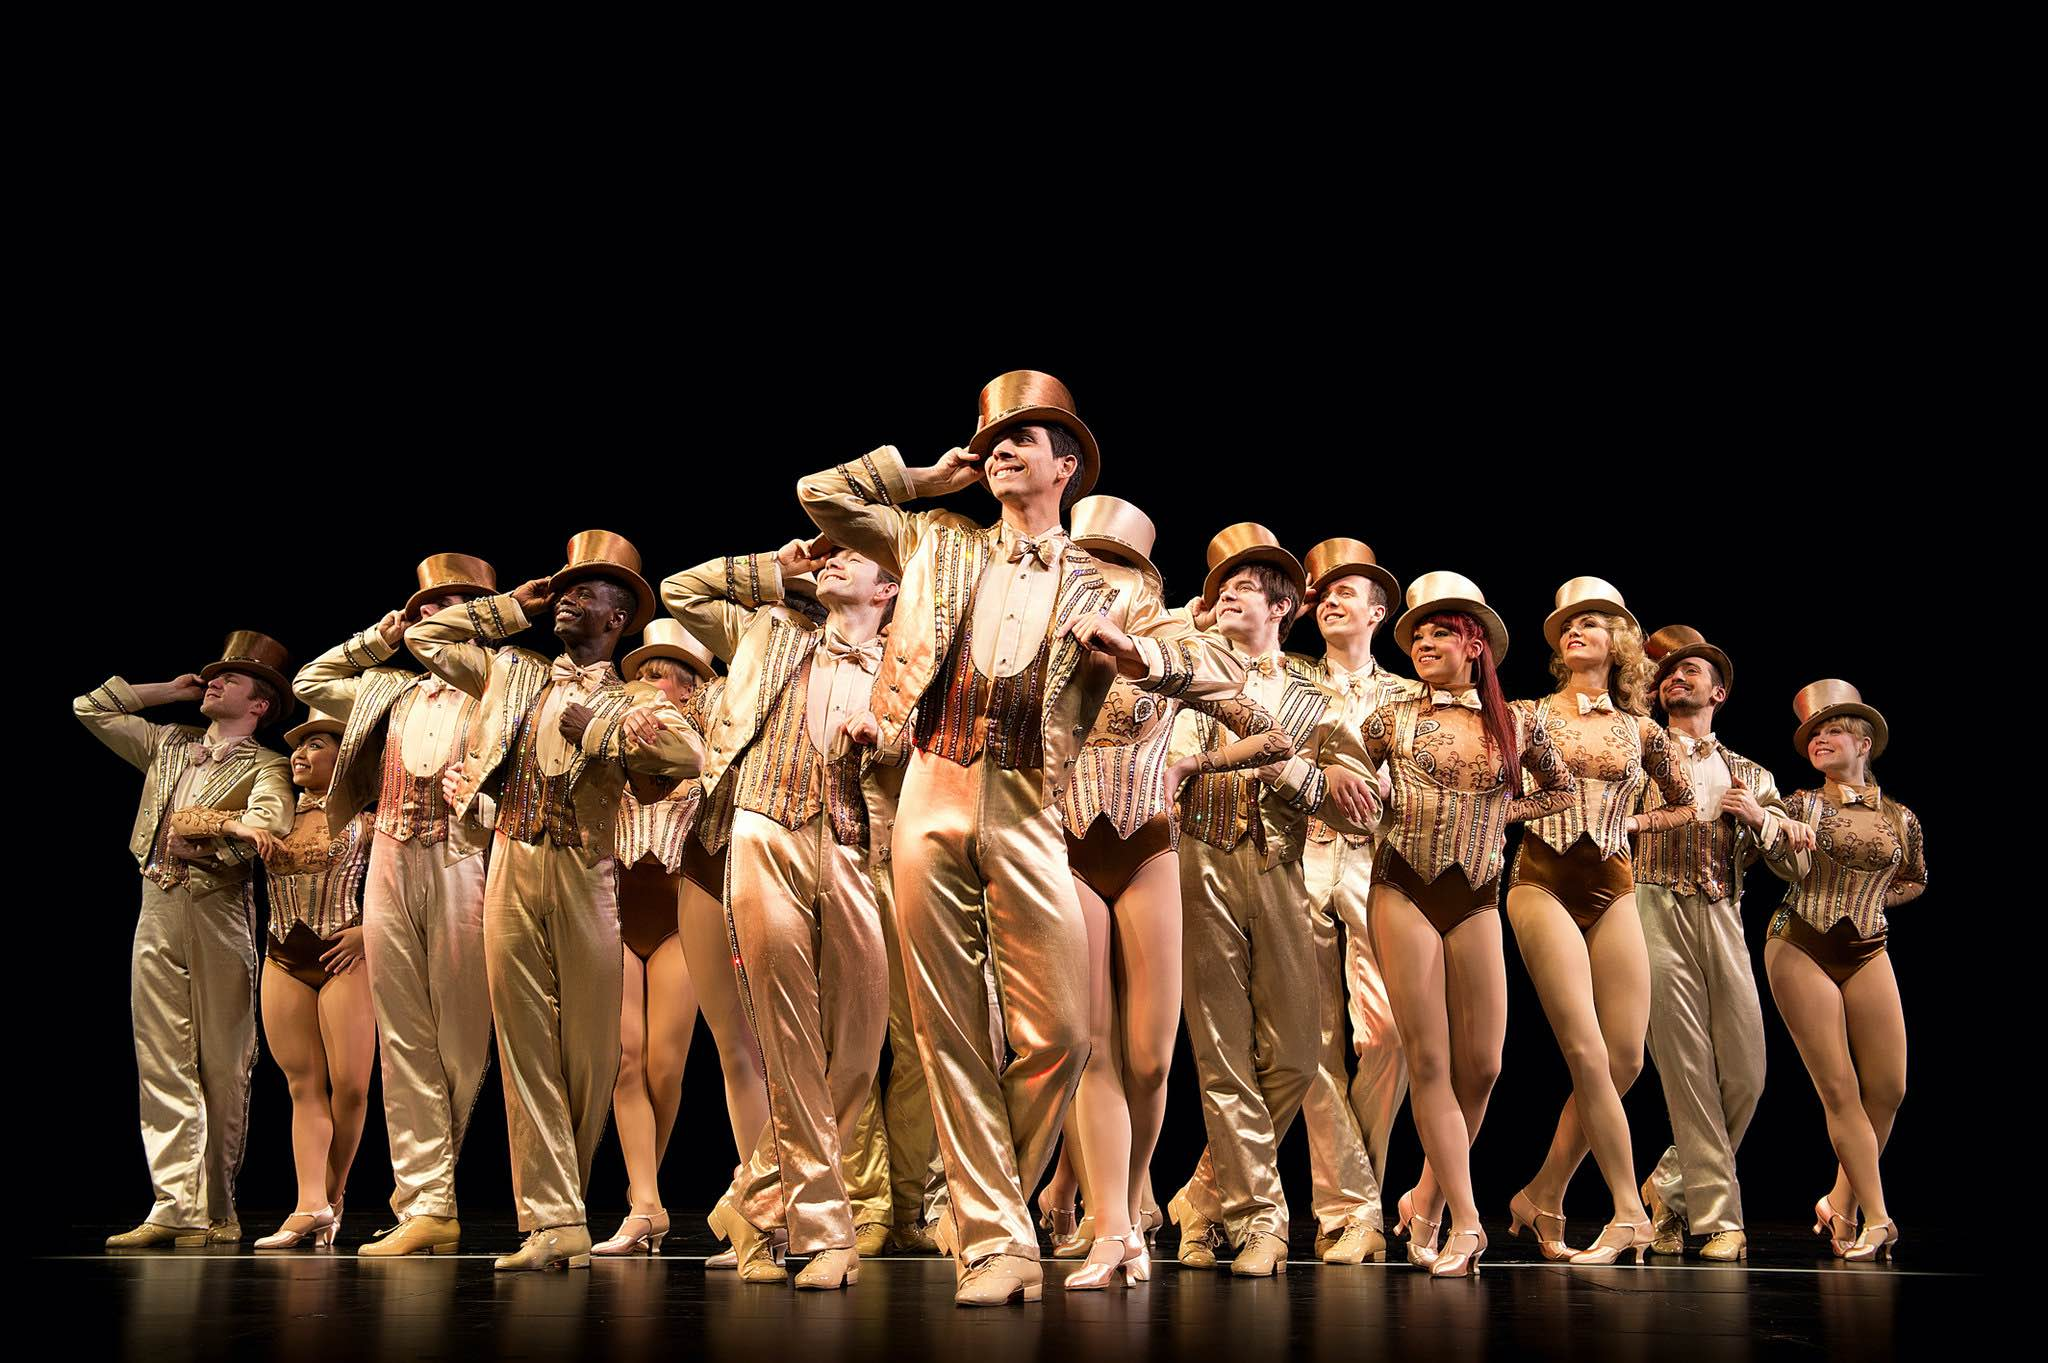
\includegraphics[max width=0.95\textwidth,
        max height=0.58000\textheight]{{Images/chorusline}.jpg}
    \end{center}
    \end{column}
    \end{columns}
}
\end{frame}
\begin{frame}[t]{Broadway Musical Names from Song Titles, Answer 7}
% \vspace{0.5em}
\begin{block}{Question}
Out Tonight
\end{block}

\visible<2->{
    \begin{columns}[T,totalwidth=\linewidth]
    \begin{column}{0.32\linewidth}
    \begin{block}{Answer}
    \emph{Rent}
    \end{block}
    \end{column}
    \begin{column}{0.65\linewidth}
    \begin{center}
    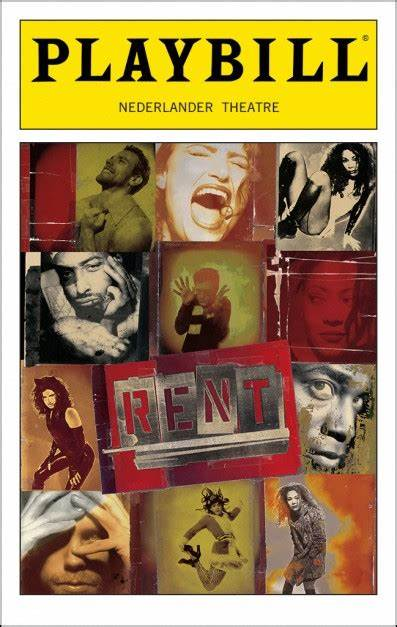
\includegraphics[max width=0.95\textwidth,
        max height=0.58000\textheight]{{Images/rent}.jpeg}
    \end{center}
    \end{column}
    \end{columns}
}
\end{frame}
\begin{frame}[t]{Broadway Musical Names from Song Titles, Answer 8}
% \vspace{0.5em}
\begin{block}{Question}
The King of Broadway
\end{block}

\visible<2->{
    \begin{columns}[T,totalwidth=\linewidth]
    \begin{column}{0.32\linewidth}
    \begin{block}{Answer}
    \emph{The Producers}
    \end{block}
    \end{column}
    \begin{column}{0.65\linewidth}
    \begin{center}
    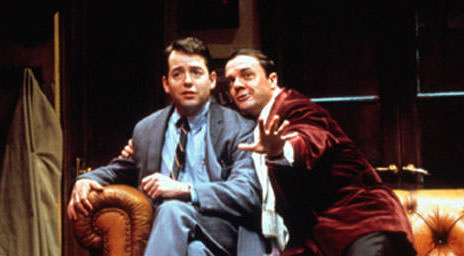
\includegraphics[max width=0.95\textwidth,
        max height=0.58000\textheight]{{Images/producers}.jpg}
    \end{center}
    \end{column}
    \end{columns}
}
\end{frame}
\begin{frame}[t]{Broadway Musical Names from Song Titles, Answer 9}
% \vspace{0.5em}
\begin{block}{Question}
Cool
\end{block}

\visible<2->{
    \begin{columns}[T,totalwidth=\linewidth]
    \begin{column}{0.32\linewidth}
    \begin{block}{Answer}
    \emph{West Side Story}
    \end{block}
    \end{column}
    \begin{column}{0.65\linewidth}
    \begin{center}
    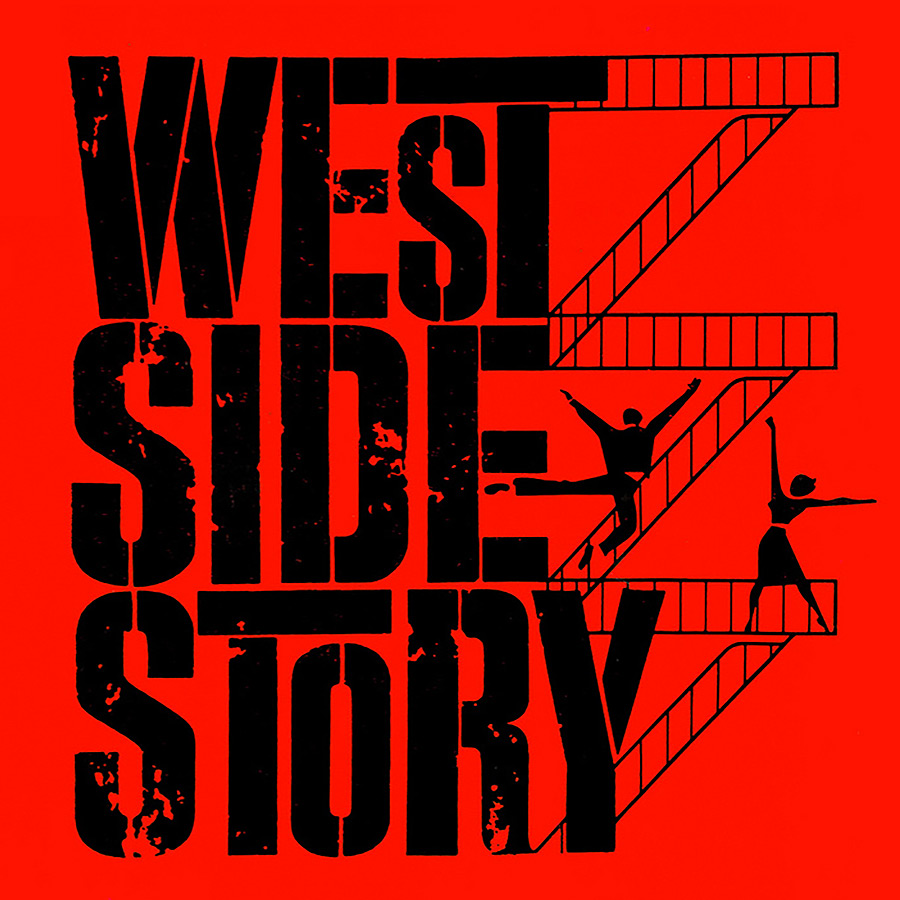
\includegraphics[max width=0.95\textwidth,
        max height=0.58000\textheight]{{Images/westsidestory}.jpg}
    \end{center}
    \end{column}
    \end{columns}
}
\end{frame}
\begin{frame}[t]{Broadway Musical Names from Song Titles, Answer 10}
% \vspace{0.5em}
\begin{block}{Question}
It Might as Well be Spring
\end{block}

\visible<2->{
    \begin{columns}[T,totalwidth=\linewidth]
    \begin{column}{0.32\linewidth}
    \begin{block}{Answer}
    \emph{State Fair}
    \end{block}
    \end{column}
    \begin{column}{0.65\linewidth}
    \begin{center}
    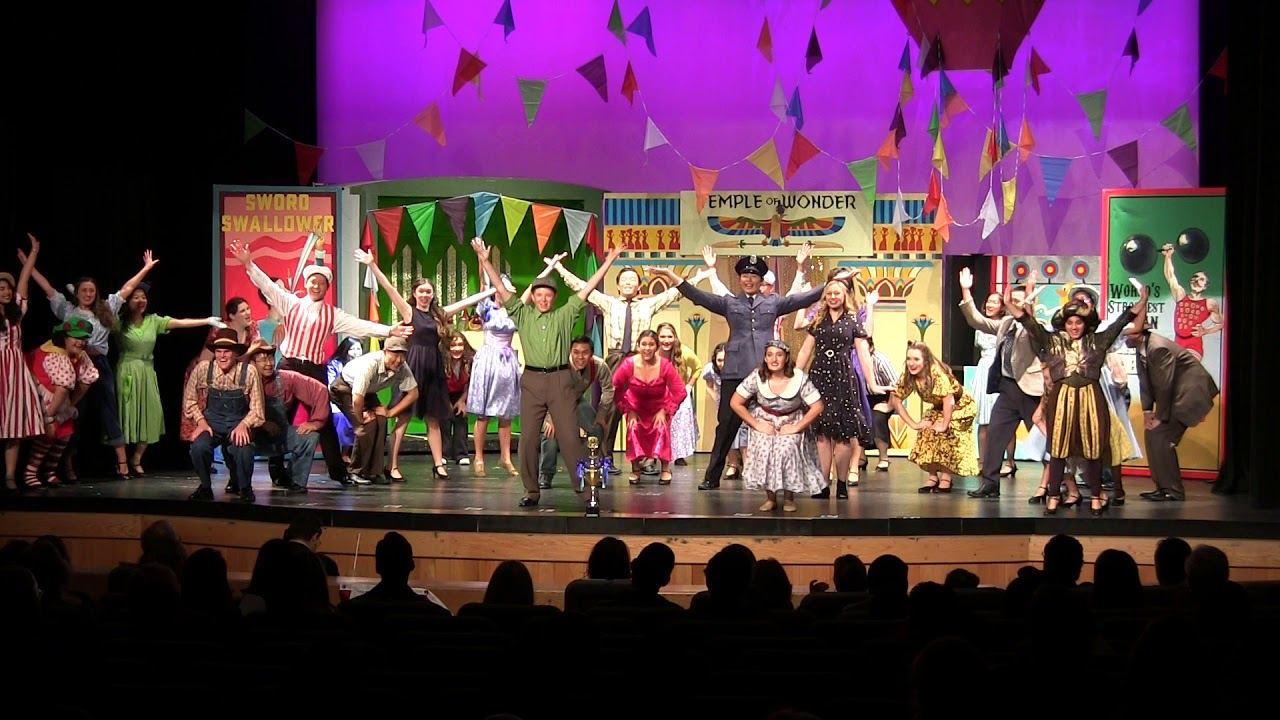
\includegraphics[max width=0.95\textwidth,
        max height=0.58000\textheight]{{Images/statefair}.jpg}
    \end{center}
    \end{column}
    \end{columns}
}
\end{frame}
\def\thisSectionName{Dog Breeds}
\section{Round 4}
\subsection*{Q1}
\begin{frame}[t]{Dog Breeds, Question 1}
% \vspace{0.5em}
\begin{columns}[T,totalwidth=\linewidth]
\begin{column}{0.32\linewidth}
\begin{block}{Question}
Name the breed.
\end{block}
\end{column}
\begin{column}{0.65\linewidth}
\begin{center}
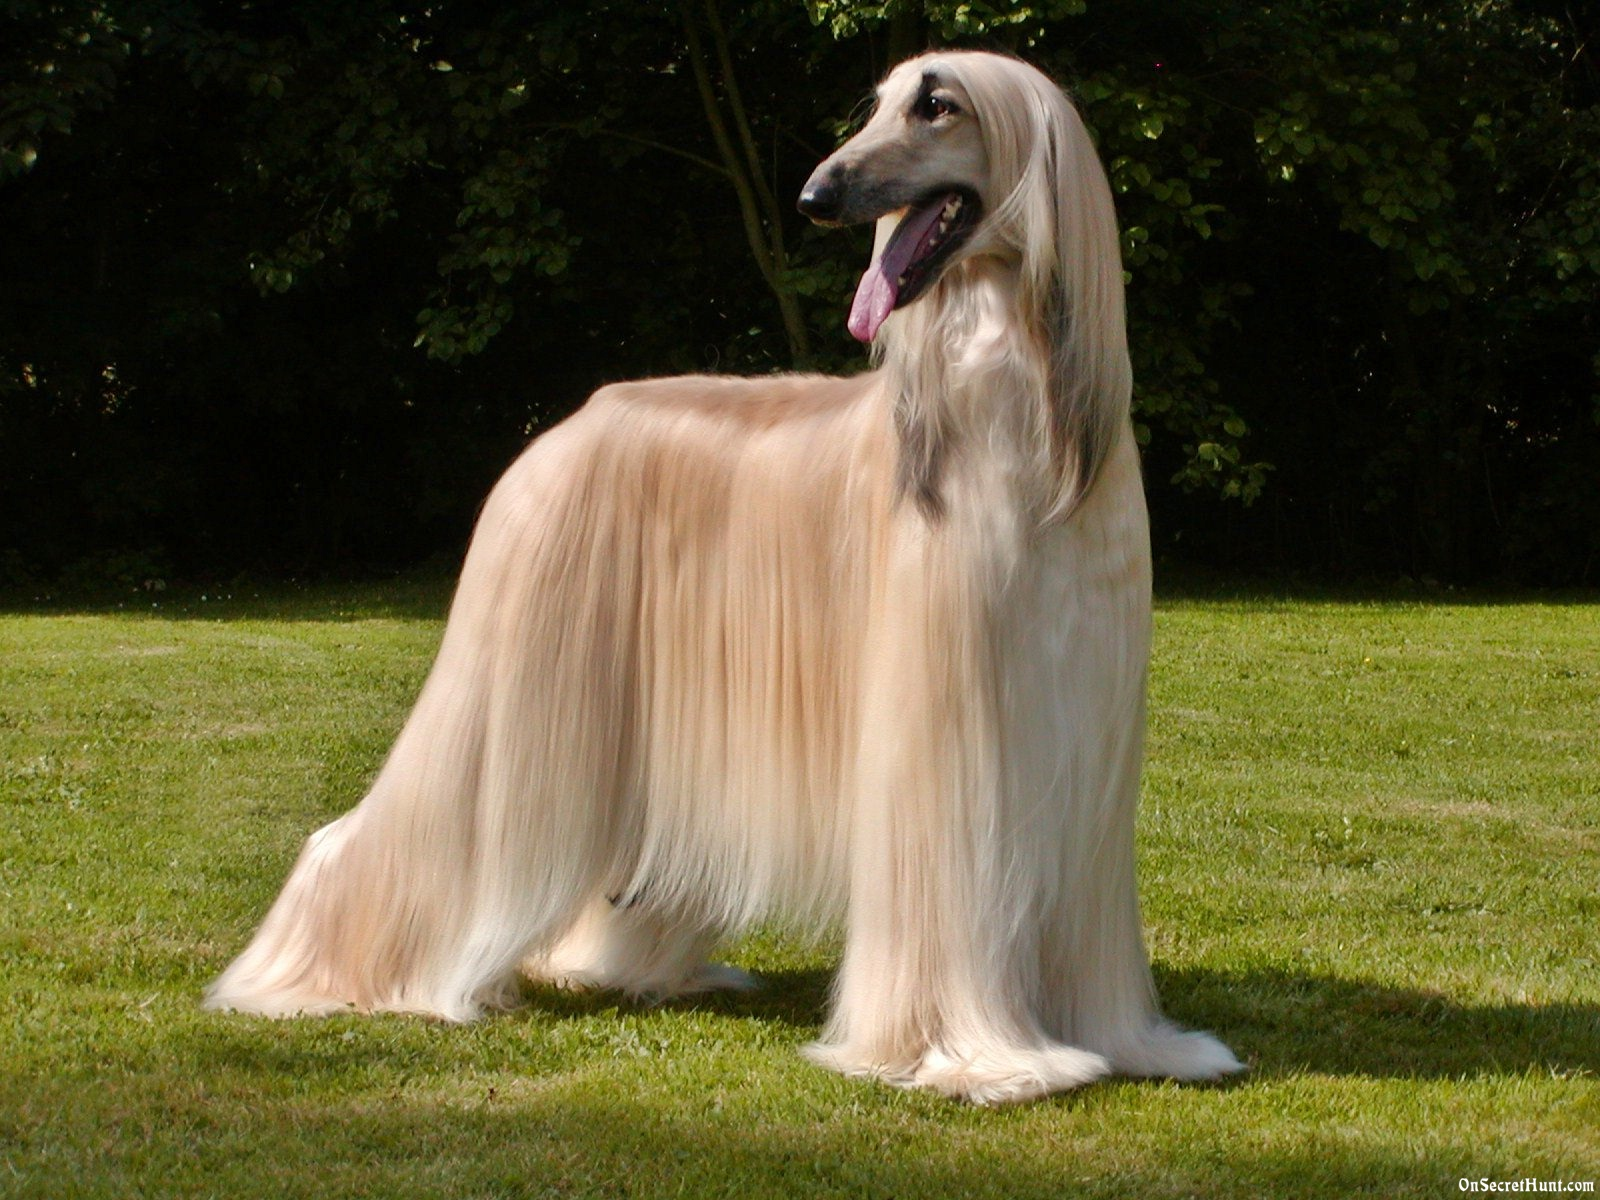
\includegraphics[max width=0.95\textwidth,max height=0.7\textheight]{{Images/afghanhound}.jpg}
\end{center}
\end{column}
\end{columns}
\end{frame}
\subsection*{Q2}
\begin{frame}[t]{Dog Breeds, Question 2}
% \vspace{0.5em}
\begin{columns}[T,totalwidth=\linewidth]
\begin{column}{0.32\linewidth}
\begin{block}{Question}
Name the breed.
\end{block}
\end{column}
\begin{column}{0.65\linewidth}
\begin{center}
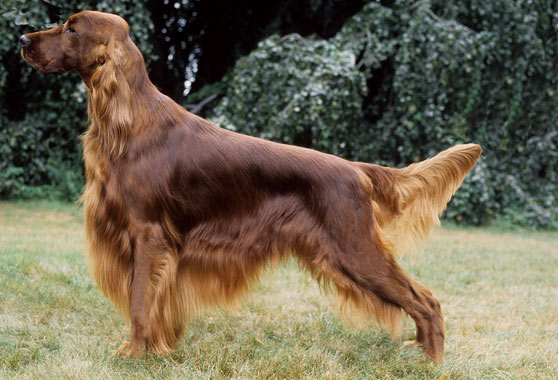
\includegraphics[max width=0.95\textwidth,max height=0.7\textheight]{{Images/irishsetter}.jpg}
\end{center}
\end{column}
\end{columns}
\end{frame}
\subsection*{Q3}
\begin{frame}[t]{Dog Breeds, Question 3}
% \vspace{0.5em}
\begin{columns}[T,totalwidth=\linewidth]
\begin{column}{0.32\linewidth}
\begin{block}{Question}
Name the breed.
\end{block}
\end{column}
\begin{column}{0.65\linewidth}
\begin{center}
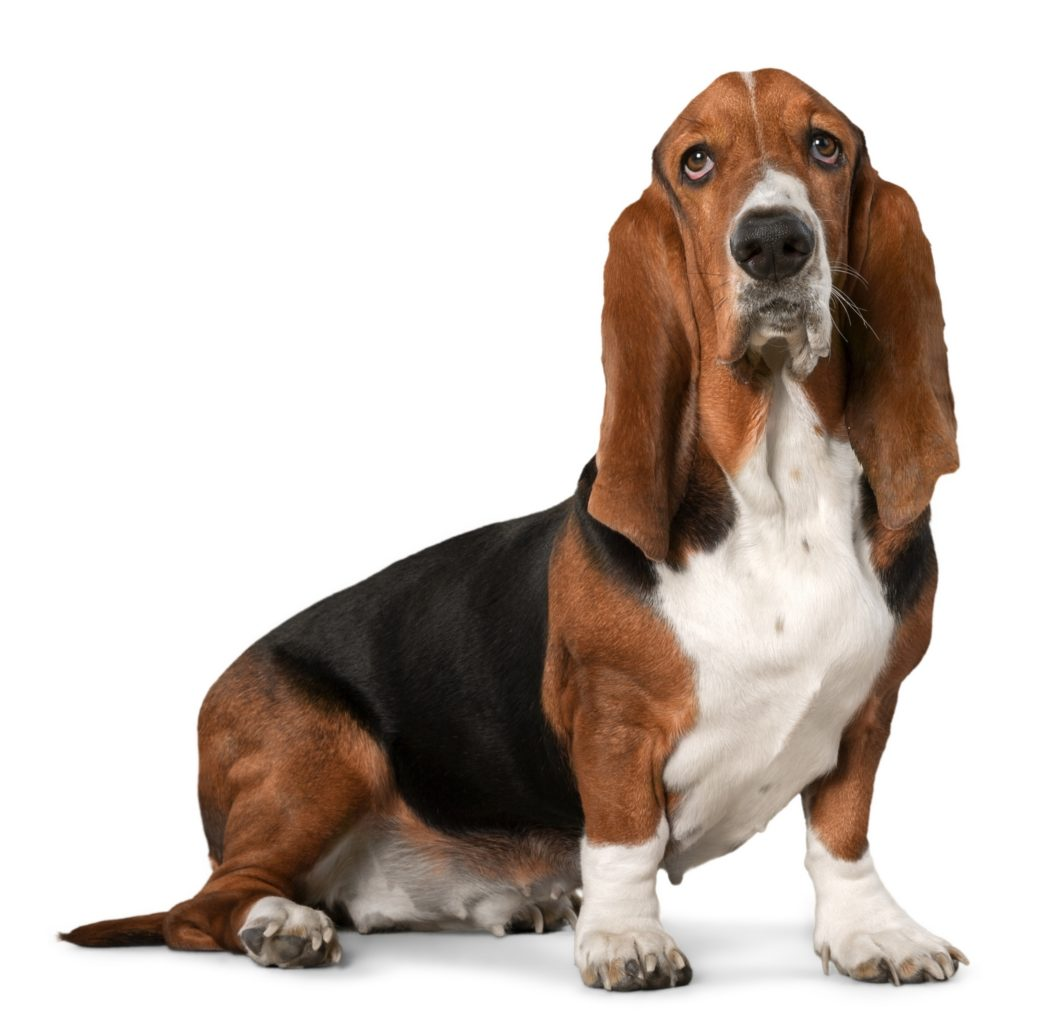
\includegraphics[max width=0.95\textwidth,max height=0.7\textheight]{{Images/bassethound}.jpg}
\end{center}
\end{column}
\end{columns}
\end{frame}
\subsection*{Q4}
\begin{frame}[t]{Dog Breeds, Question 4}
% \vspace{0.5em}
\begin{columns}[T,totalwidth=\linewidth]
\begin{column}{0.32\linewidth}
\begin{block}{Question}
Name the breed.
\end{block}
\end{column}
\begin{column}{0.65\linewidth}
\begin{center}
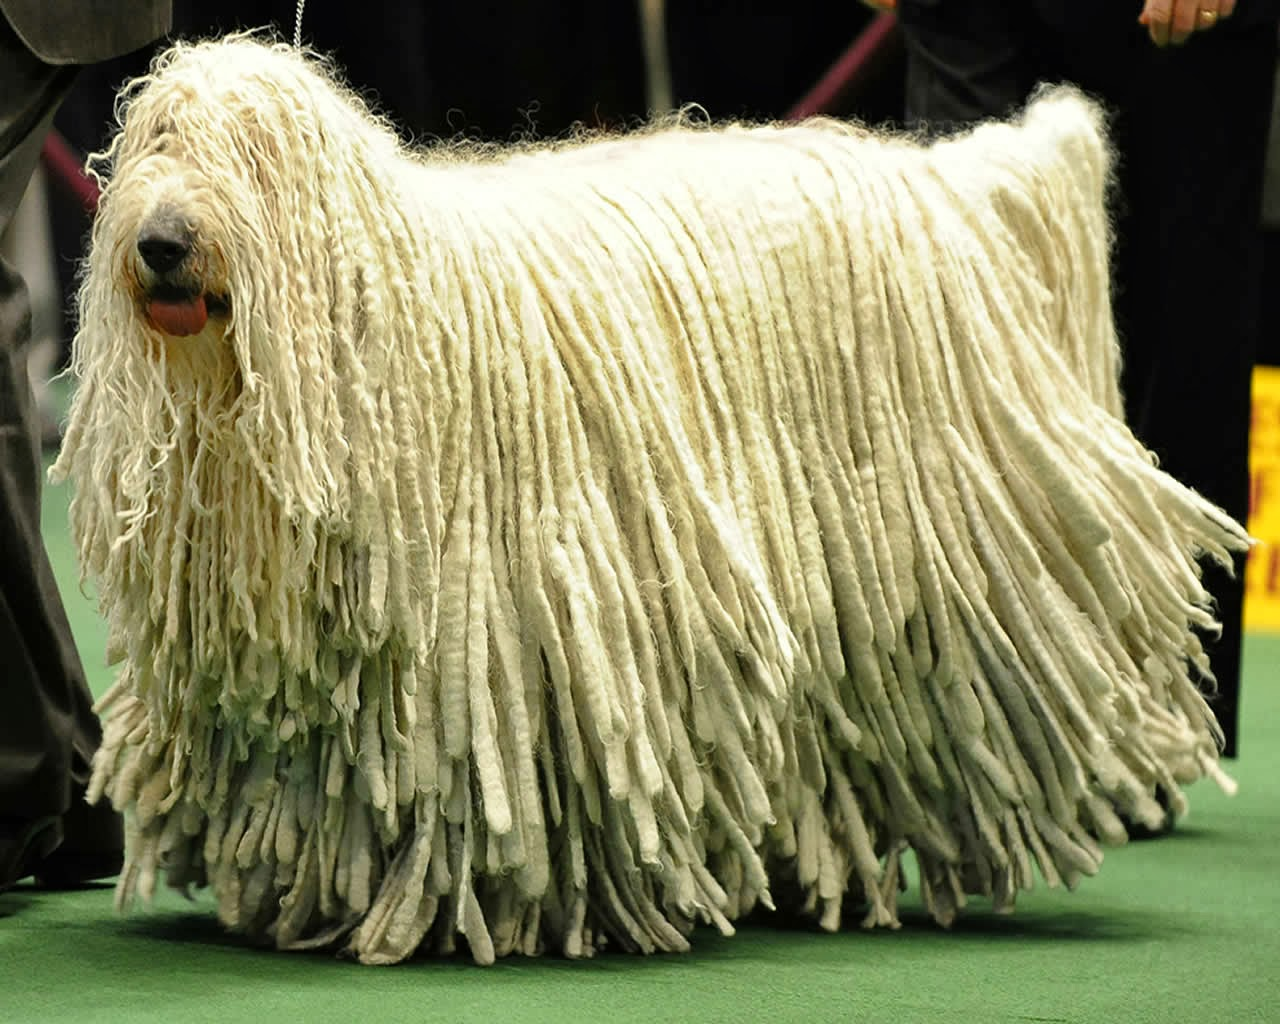
\includegraphics[max width=0.95\textwidth,max height=0.7\textheight]{{Images/komondor}.jpg}
\end{center}
\end{column}
\end{columns}
\end{frame}
\subsection*{Q5}
\begin{frame}[t]{Dog Breeds, Question 5}
% \vspace{0.5em}
\begin{columns}[T,totalwidth=\linewidth]
\begin{column}{0.32\linewidth}
\begin{block}{Question}
Name the breed.
\end{block}
\end{column}
\begin{column}{0.65\linewidth}
\begin{center}
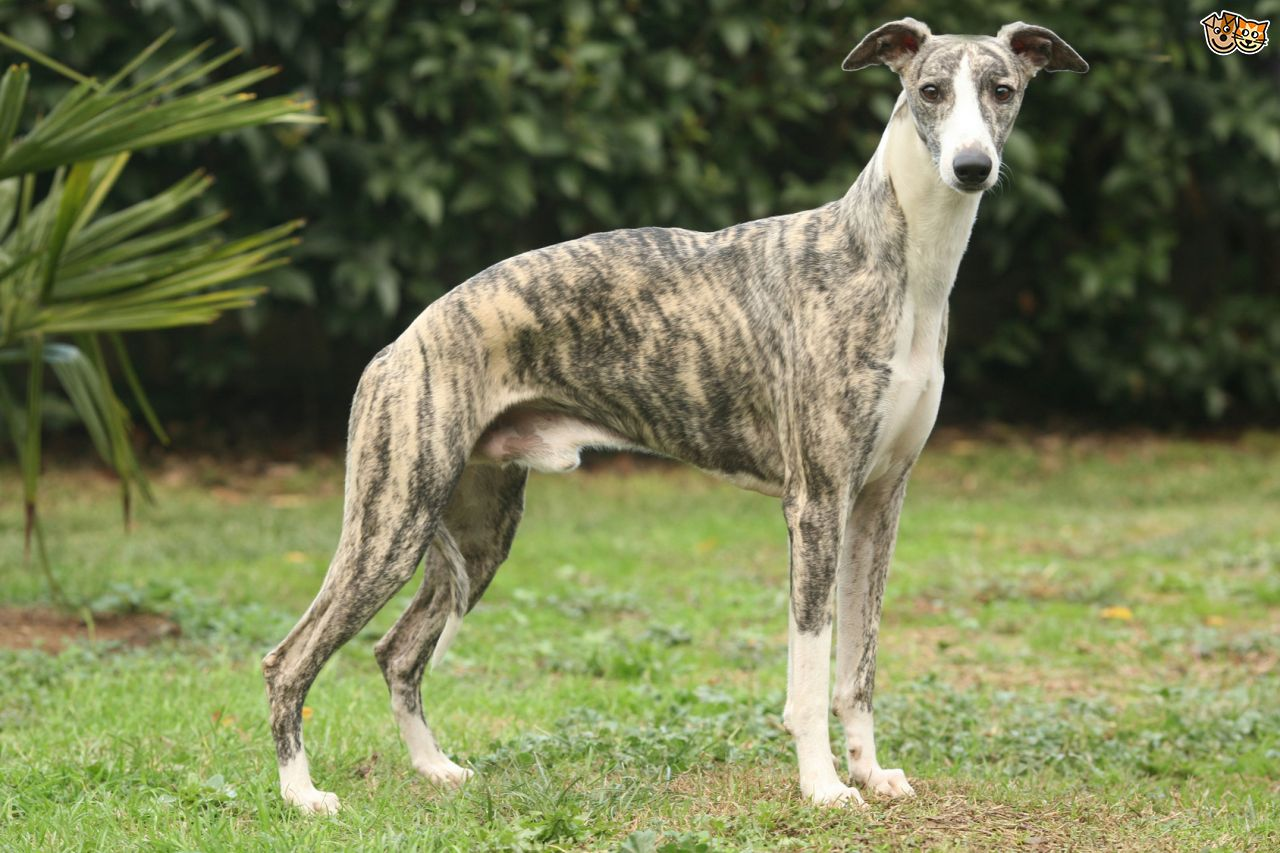
\includegraphics[max width=0.95\textwidth,max height=0.7\textheight]{{Images/whippet}.jpg}
\end{center}
\end{column}
\end{columns}
\end{frame}
\subsection*{Q6}
\begin{frame}[t]{Dog Breeds, Question 6}
% \vspace{0.5em}
\begin{columns}[T,totalwidth=\linewidth]
\begin{column}{0.32\linewidth}
\begin{block}{Question}
Name the breed.
\end{block}
\end{column}
\begin{column}{0.65\linewidth}
\begin{center}
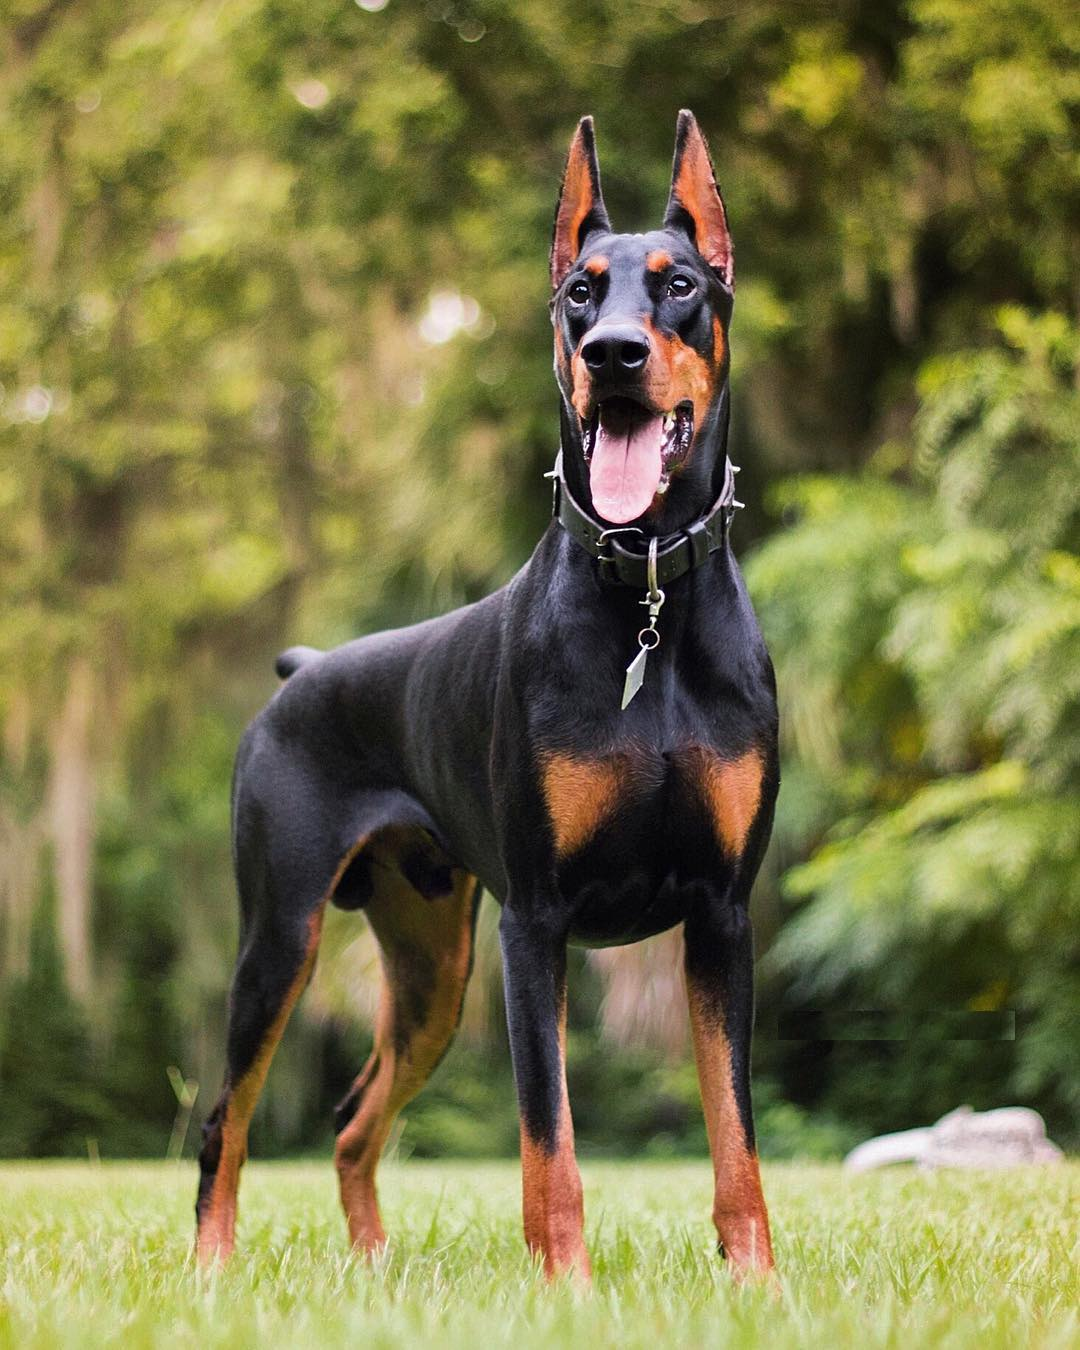
\includegraphics[max width=0.95\textwidth,max height=0.7\textheight]{{Images/doberman}.jpg}
\end{center}
\end{column}
\end{columns}
\end{frame}
\subsection*{Q7}
\begin{frame}[t]{Dog Breeds, Question 7}
% \vspace{0.5em}
\begin{columns}[T,totalwidth=\linewidth]
\begin{column}{0.32\linewidth}
\begin{block}{Question}
Name the breed.
\end{block}
\end{column}
\begin{column}{0.65\linewidth}
\begin{center}
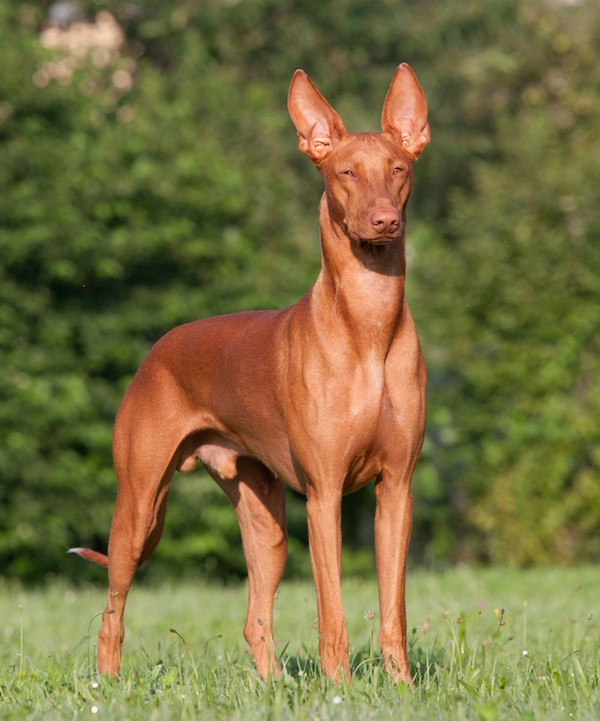
\includegraphics[max width=0.95\textwidth,max height=0.7\textheight]{{Images/pharaohhound}.jpg}
\end{center}
\end{column}
\end{columns}
\end{frame}
\subsection*{Q8}
\begin{frame}[t]{Dog Breeds, Question 8}
% \vspace{0.5em}
\begin{columns}[T,totalwidth=\linewidth]
\begin{column}{0.32\linewidth}
\begin{block}{Question}
Name the breed.
\end{block}
\end{column}
\begin{column}{0.65\linewidth}
\begin{center}
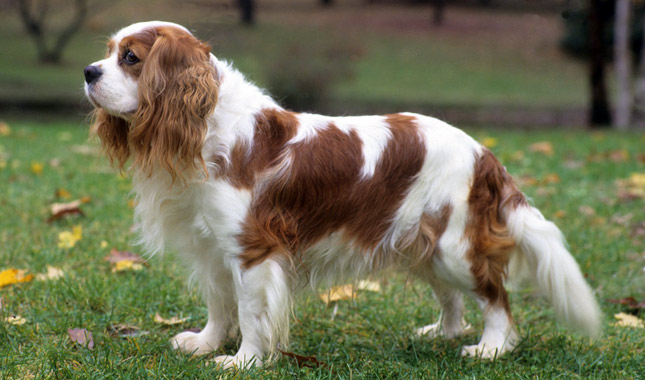
\includegraphics[max width=0.95\textwidth,max height=0.7\textheight]{{Images/ckcs}.jpg}
\end{center}
\end{column}
\end{columns}
\end{frame}
\subsection*{Q9}
\begin{frame}[t]{Dog Breeds, Question 9}
% \vspace{0.5em}
\begin{columns}[T,totalwidth=\linewidth]
\begin{column}{0.32\linewidth}
\begin{block}{Question}
Name the breed.
\end{block}
\end{column}
\begin{column}{0.65\linewidth}
\begin{center}
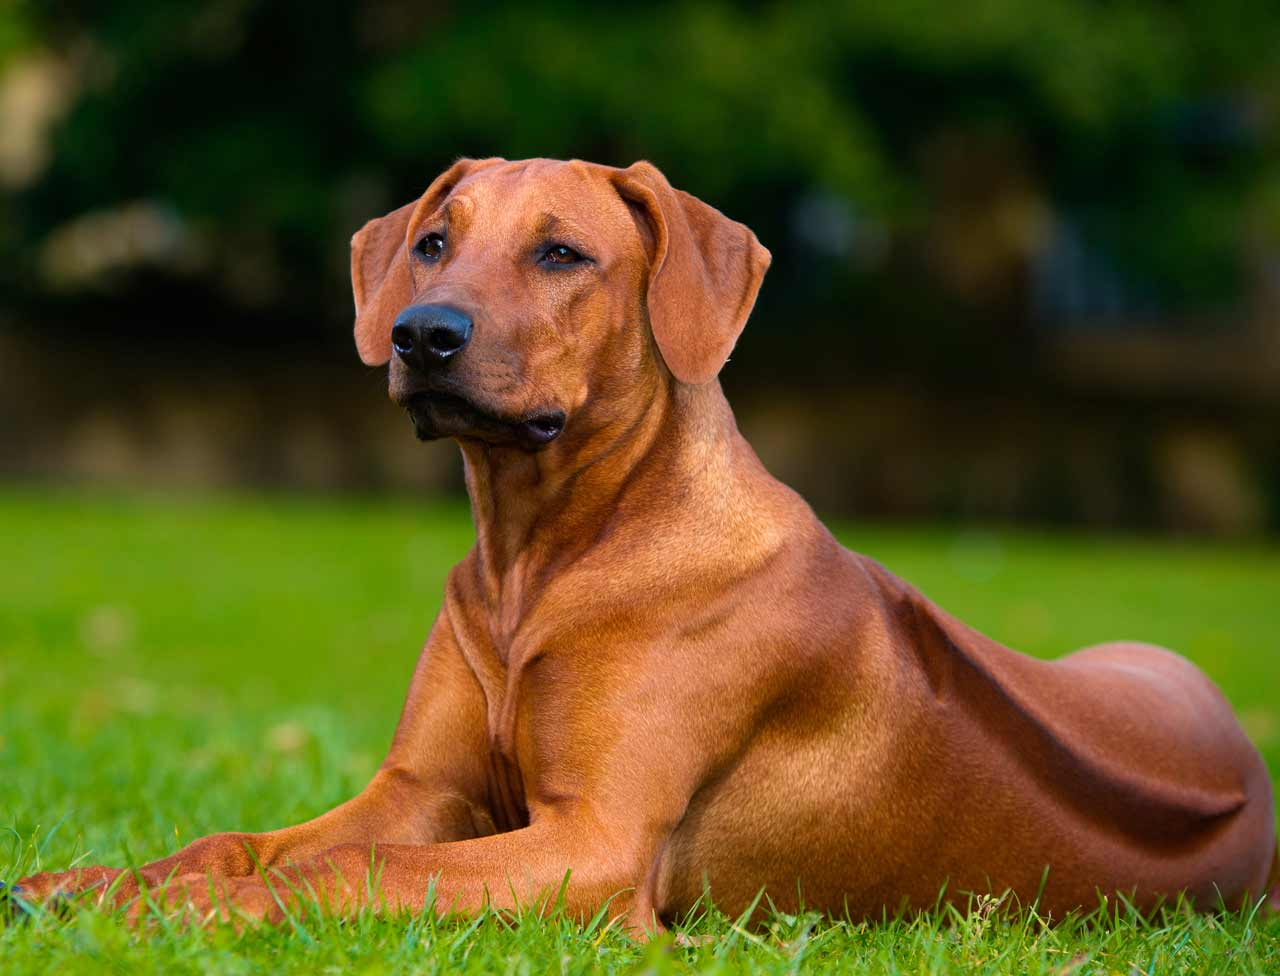
\includegraphics[max width=0.95\textwidth,max height=0.7\textheight]{{Images/rhodesianridgeback}.jpg}
\end{center}
\end{column}
\end{columns}
\end{frame}
\subsection*{Q10}
\begin{frame}[t]{Dog Breeds, Question 10}
% \vspace{0.5em}
\begin{columns}[T,totalwidth=\linewidth]
\begin{column}{0.32\linewidth}
\begin{block}{Question}
Name the breed.
\end{block}
\end{column}
\begin{column}{0.65\linewidth}
\begin{center}
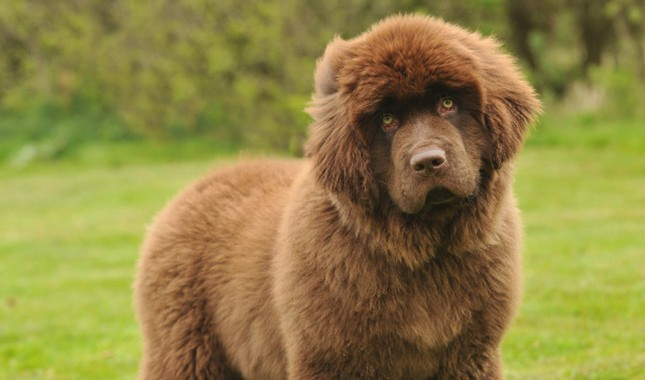
\includegraphics[max width=0.95\textwidth,max height=0.7\textheight]{{Images/newfoundland}.jpeg}
\end{center}
\end{column}
\end{columns}
\end{frame}
\subsection{Answers}
\begin{frame}[t]{Dog Breeds, Answer 1}
% \vspace{0.5em}
\begin{columns}[T,totalwidth=\linewidth]
\begin{column}{0.32\linewidth}
\begin{block}{Question}
Name the breed.
\end{block}
\visible<2->{
    \begin{block}{Answer}
    Afghan hound
    \end{block}
}
\end{column}
\begin{column}{0.65\linewidth}
\begin{center}
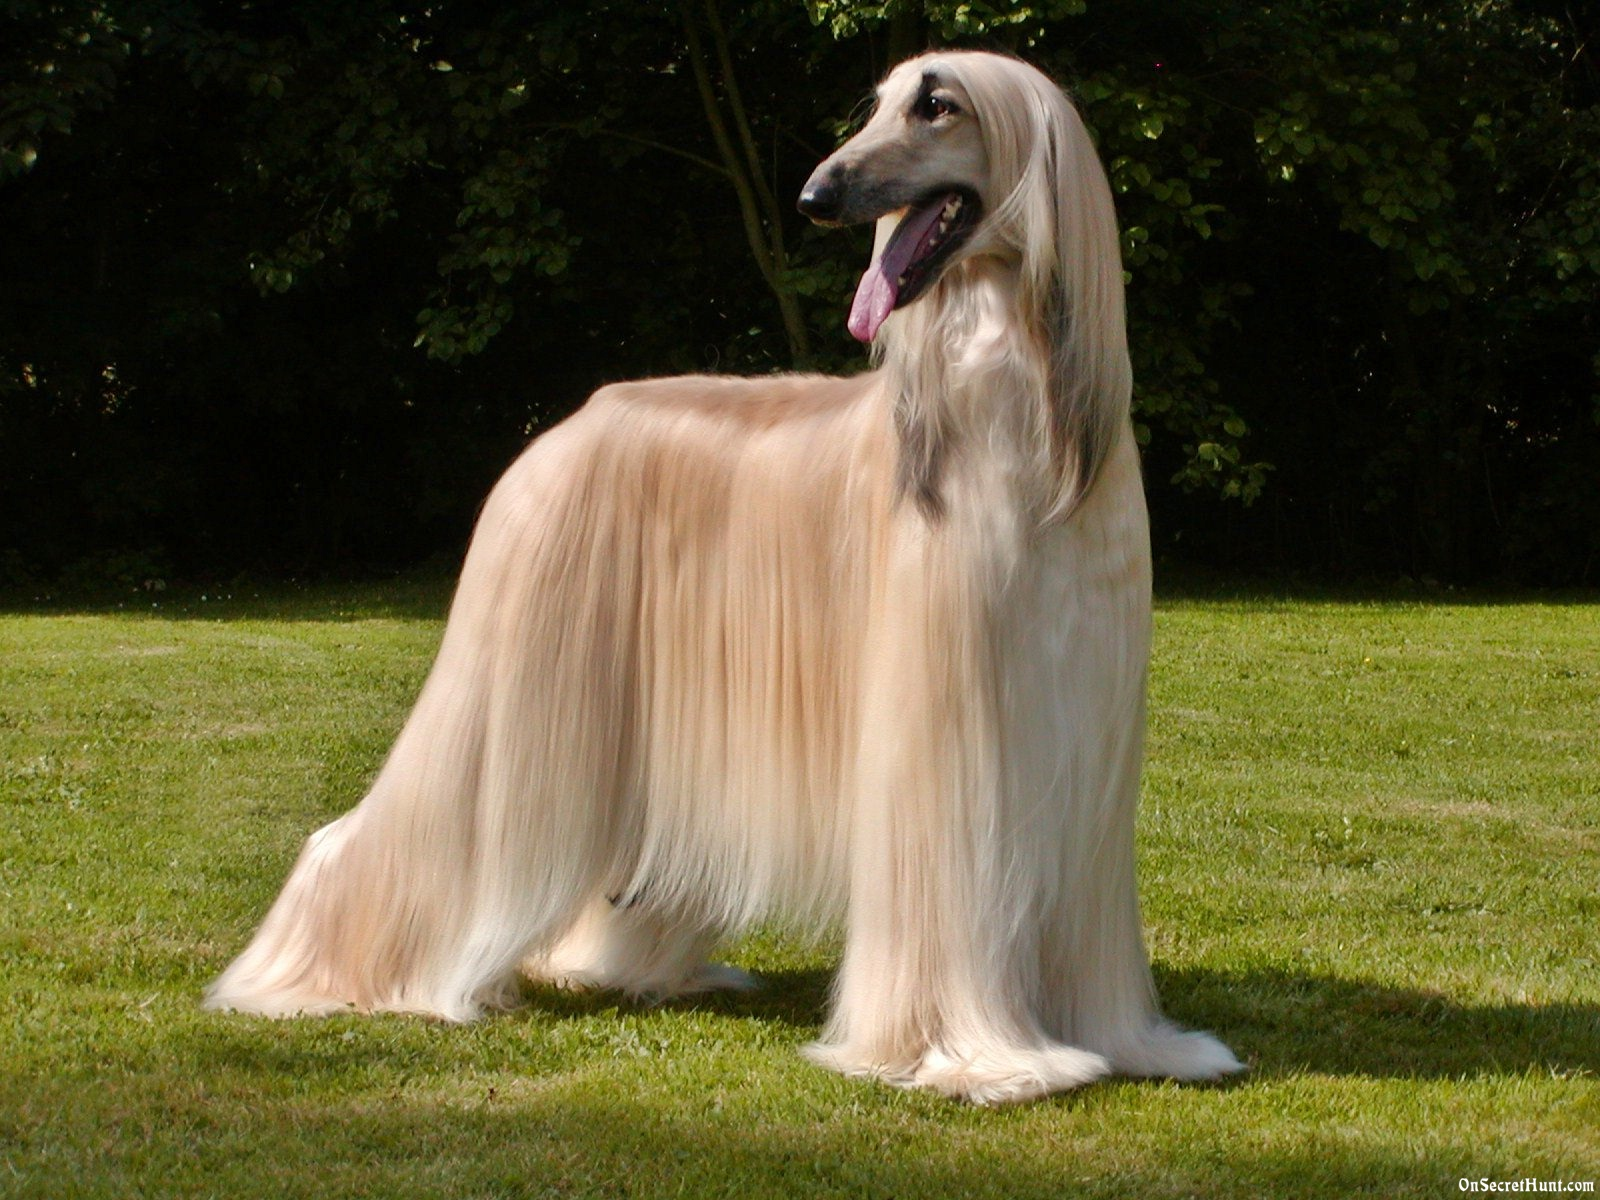
\includegraphics[max width=0.95\textwidth,max height=0.7\textheight]{{Images/afghanhound}.jpg}
\end{center}
\end{column}
\end{columns}
\end{frame}
\begin{frame}[t]{Dog Breeds, Answer 2}
% \vspace{0.5em}
\begin{columns}[T,totalwidth=\linewidth]
\begin{column}{0.32\linewidth}
\begin{block}{Question}
Name the breed.
\end{block}
\visible<2->{
    \begin{block}{Answer}
    Irish setter
    \end{block}
}
\end{column}
\begin{column}{0.65\linewidth}
\begin{center}
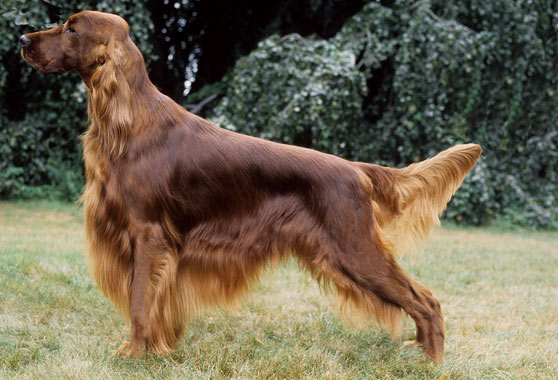
\includegraphics[max width=0.95\textwidth,max height=0.7\textheight]{{Images/irishsetter}.jpg}
\end{center}
\end{column}
\end{columns}
\end{frame}
\begin{frame}[t]{Dog Breeds, Answer 3}
% \vspace{0.5em}
\begin{columns}[T,totalwidth=\linewidth]
\begin{column}{0.32\linewidth}
\begin{block}{Question}
Name the breed.
\end{block}
\visible<2->{
    \begin{block}{Answer}
    Basset hound
    \end{block}
}
\end{column}
\begin{column}{0.65\linewidth}
\begin{center}
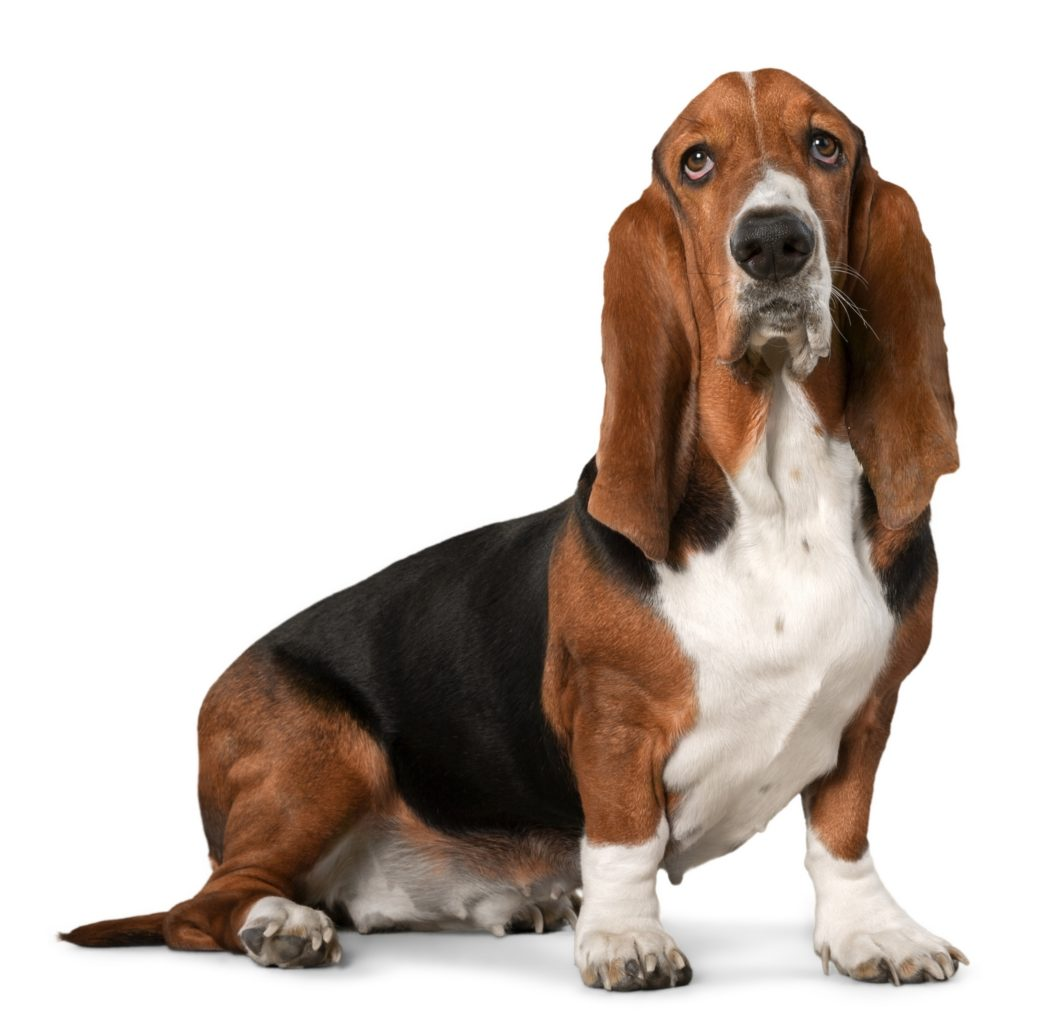
\includegraphics[max width=0.95\textwidth,max height=0.7\textheight]{{Images/bassethound}.jpg}
\end{center}
\end{column}
\end{columns}
\end{frame}
\begin{frame}[t]{Dog Breeds, Answer 4}
% \vspace{0.5em}
\begin{columns}[T,totalwidth=\linewidth]
\begin{column}{0.32\linewidth}
\begin{block}{Question}
Name the breed.
\end{block}
\visible<2->{
    \begin{block}{Answer}
    Komondor (but we'll also accept Puli)
    \end{block}
}
\end{column}
\begin{column}{0.65\linewidth}
\begin{center}
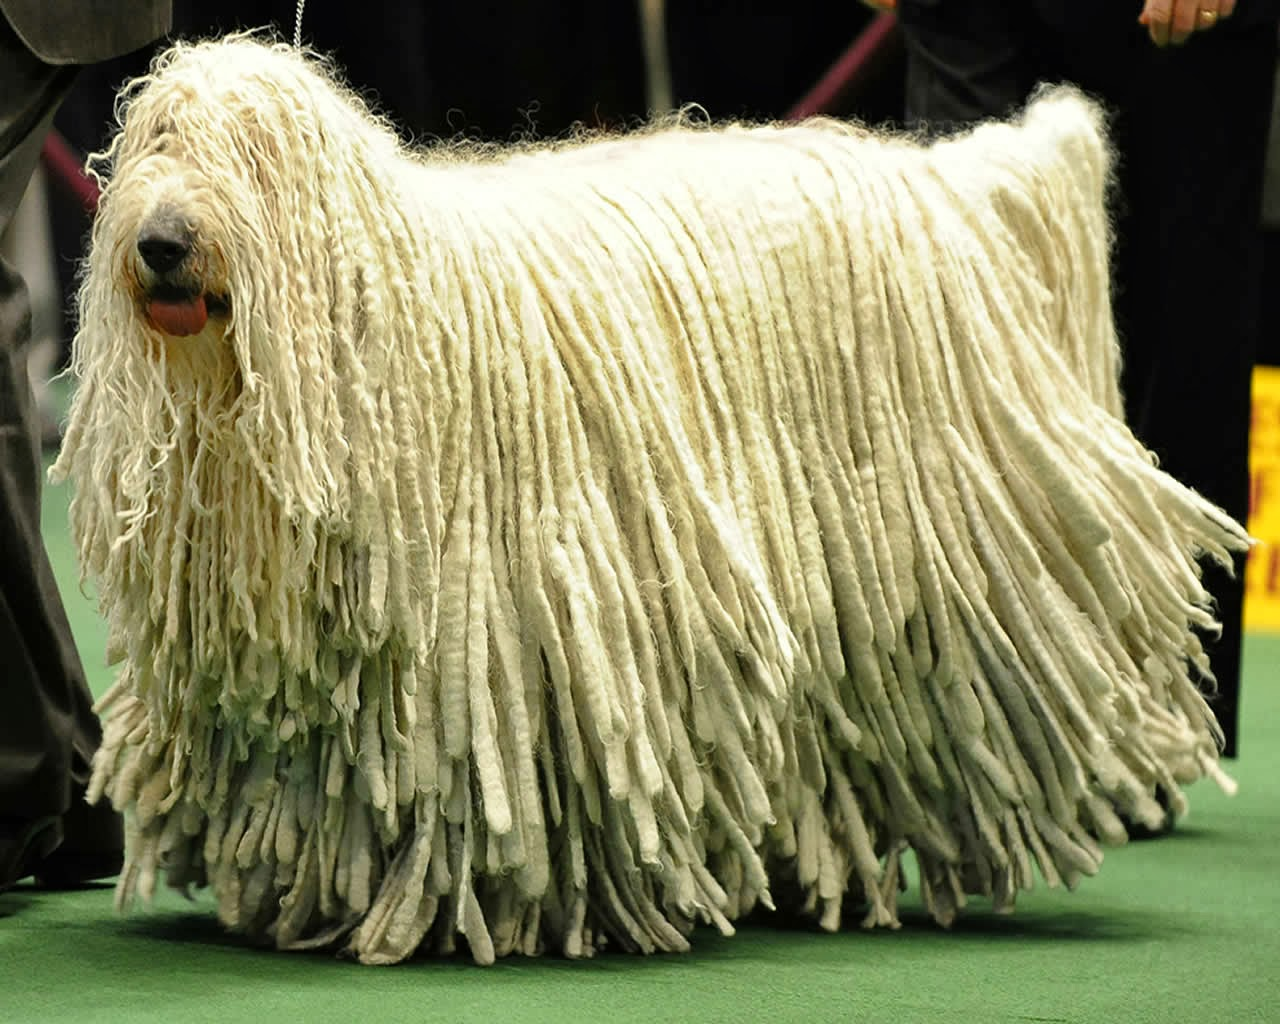
\includegraphics[max width=0.95\textwidth,max height=0.7\textheight]{{Images/komondor}.jpg}
\end{center}
\end{column}
\end{columns}
\end{frame}
\begin{frame}[t]{Dog Breeds, Answer 5}
% \vspace{0.5em}
\begin{columns}[T,totalwidth=\linewidth]
\begin{column}{0.32\linewidth}
\begin{block}{Question}
Name the breed.
\end{block}
\visible<2->{
    \begin{block}{Answer}
    Whippet
    \end{block}
}
\end{column}
\begin{column}{0.65\linewidth}
\begin{center}
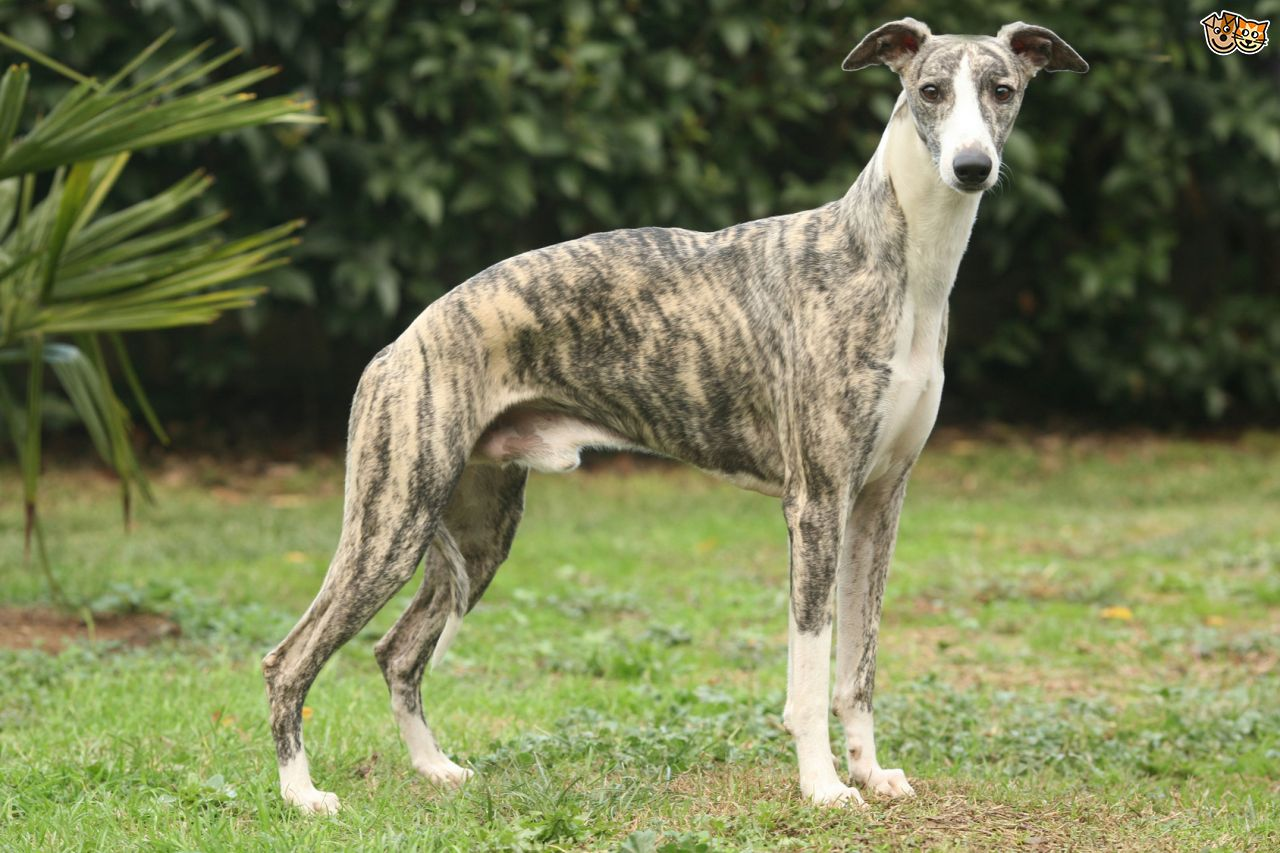
\includegraphics[max width=0.95\textwidth,max height=0.7\textheight]{{Images/whippet}.jpg}
\end{center}
\end{column}
\end{columns}
\end{frame}
\begin{frame}[t]{Dog Breeds, Answer 6}
% \vspace{0.5em}
\begin{columns}[T,totalwidth=\linewidth]
\begin{column}{0.32\linewidth}
\begin{block}{Question}
Name the breed.
\end{block}
\visible<2->{
    \begin{block}{Answer}
    Doberman Pinscher
    \end{block}
}
\end{column}
\begin{column}{0.65\linewidth}
\begin{center}
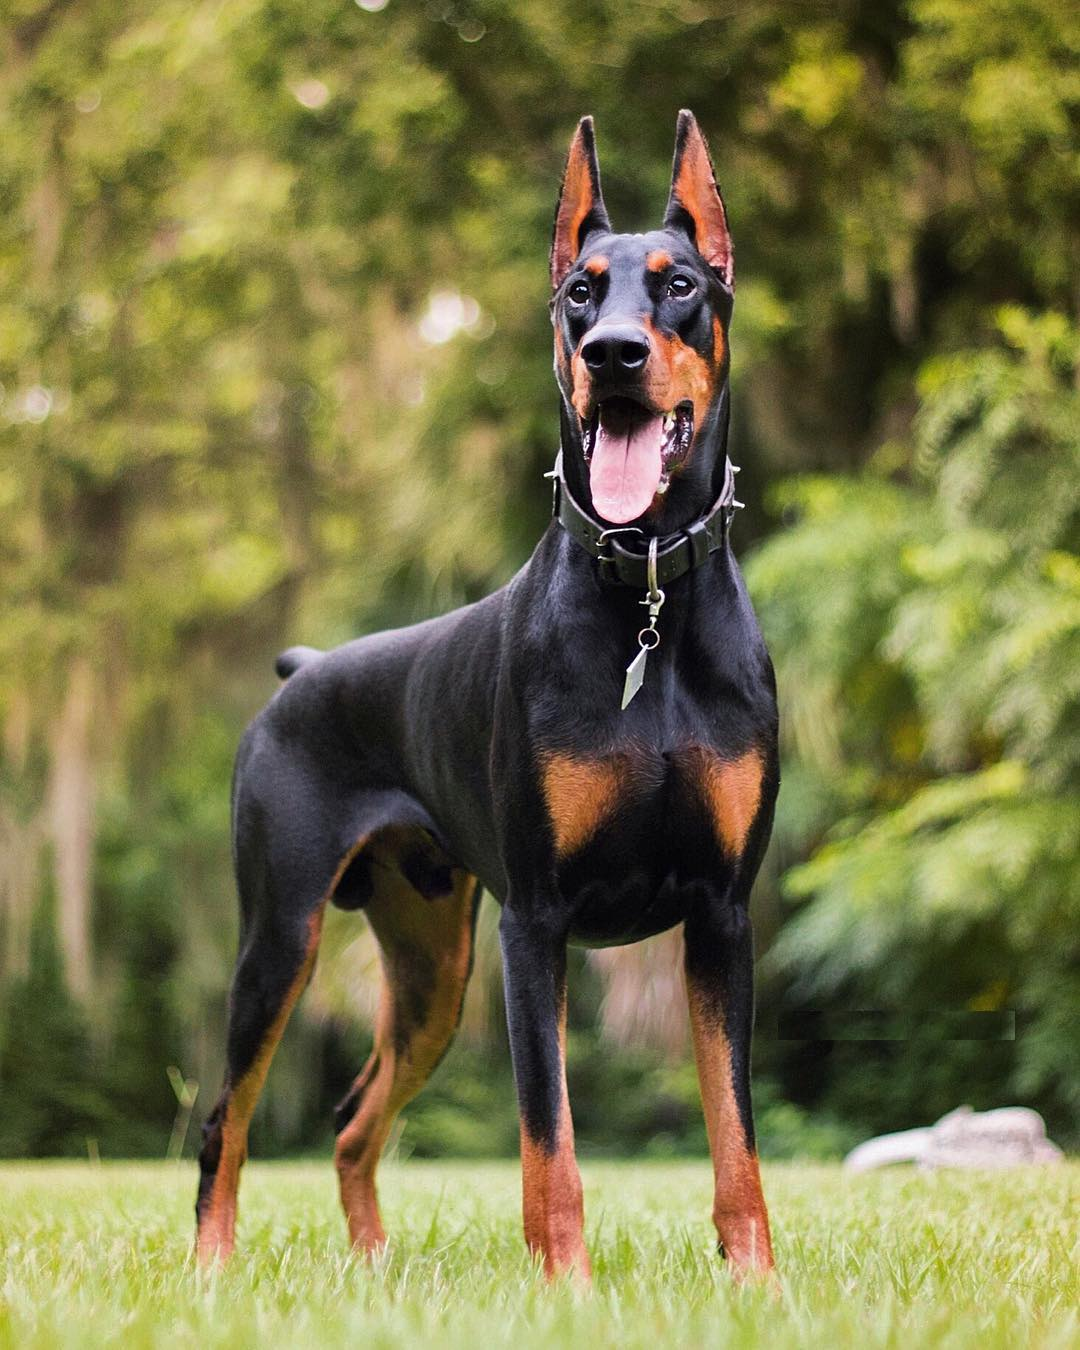
\includegraphics[max width=0.95\textwidth,max height=0.7\textheight]{{Images/doberman}.jpg}
\end{center}
\end{column}
\end{columns}
\end{frame}
\begin{frame}[t]{Dog Breeds, Answer 7}
% \vspace{0.5em}
\begin{columns}[T,totalwidth=\linewidth]
\begin{column}{0.32\linewidth}
\begin{block}{Question}
Name the breed.
\end{block}
\visible<2->{
    \begin{block}{Answer}
    Pharaoh hound
    \end{block}
}
\end{column}
\begin{column}{0.65\linewidth}
\begin{center}
\includegraphics[max width=0.95\textwidth,max height=0.7\textheight]{{Images/pharaohhound}.jpg}
\end{center}
\end{column}
\end{columns}
\end{frame}
\begin{frame}[t]{Dog Breeds, Answer 8}
% \vspace{0.5em}
\begin{columns}[T,totalwidth=\linewidth]
\begin{column}{0.32\linewidth}
\begin{block}{Question}
Name the breed.
\end{block}
\visible<2->{
    \begin{block}{Answer}
    Cavalier King Charles spaniel
    \end{block}
}
\end{column}
\begin{column}{0.65\linewidth}
\begin{center}
\includegraphics[max width=0.95\textwidth,max height=0.7\textheight]{{Images/ckcs}.jpg}
\end{center}
\end{column}
\end{columns}
\end{frame}
\begin{frame}[t]{Dog Breeds, Answer 9}
% \vspace{0.5em}
\begin{columns}[T,totalwidth=\linewidth]
\begin{column}{0.32\linewidth}
\begin{block}{Question}
Name the breed.
\end{block}
\visible<2->{
    \begin{block}{Answer}
    Rhodesian ridgeback 
    \end{block}
}
\end{column}
\begin{column}{0.65\linewidth}
\begin{center}
\includegraphics[max width=0.95\textwidth,max height=0.7\textheight]{{Images/rhodesianridgeback}.jpg}
\end{center}
\end{column}
\end{columns}
\end{frame}
\begin{frame}[t]{Dog Breeds, Answer 10}
% \vspace{0.5em}
\begin{columns}[T,totalwidth=\linewidth]
\begin{column}{0.32\linewidth}
\begin{block}{Question}
Name the breed.
\end{block}
\visible<2->{
    \begin{block}{Answer}
    Newfoundland
    \end{block}
}
\end{column}
\begin{column}{0.65\linewidth}
\begin{center}
\includegraphics[max width=0.95\textwidth,max height=0.7\textheight]{{Images/newfoundland}.jpeg}
\end{center}
\end{column}
\end{columns}
\end{frame}
\def\thisSectionName{Disney}
\section{Round 5}
\subsection*{Q1}
\begin{frame}[t]{Disney, Question 1}
% \vspace{0.5em}
\begin{columns}[T,totalwidth=\linewidth]
\begin{column}{0.32\linewidth}
\begin{block}{Question}
In \emph{The Lion King}, what is Simba's mother's name?
\end{block}
\end{column}
\begin{column}{0.65\linewidth}
\begin{center}
\includegraphics[max width=0.95\textwidth,max height=0.7\textheight]{{Images/sarabi}.jpeg}
\end{center}
\end{column}
\end{columns}
\end{frame}
\subsection*{Q2}
\begin{frame}[t]{Disney, Question 2}
% \vspace{0.5em}
\begin{block}{Question}
Who is the only Disney princess who has a star on the Hollywood Walk of Fame?
\end{block}
\end{frame}
\subsection*{Q3}
\begin{frame}[t]{Disney, Question 3}
% \vspace{0.5em}
\begin{columns}[T,totalwidth=\linewidth]
\begin{column}{0.32\linewidth}
\begin{block}{Question}
In \emph{The Little Mermaid}, what were the maritime-themed names of Ursula's two pet eels?
\end{block}
\end{column}
\begin{column}{0.65\linewidth}
\begin{center}
\includegraphics[max width=0.95\textwidth,max height=0.7\textheight]{{Images/flotsamjetsam}.jpg}
\end{center}
\end{column}
\end{columns}
\end{frame}
\subsection*{Q4}
\begin{frame}[t]{Disney, Question 4}
% \vspace{0.5em}
\begin{columns}[T,totalwidth=\linewidth]
\begin{column}{0.32\linewidth}
\begin{block}{Question}
In \emph{Ratatouille}, which actor voiced the main character Remy?
\end{block}
\end{column}
\begin{column}{0.65\linewidth}
\begin{center}
\includegraphics[max width=0.95\textwidth,max height=0.7\textheight]{{Images/remy}.jpg}
\end{center}
\end{column}
\end{columns}
\end{frame}
\subsection*{Q5}
\begin{frame}[t]{Disney, Question 5}
% \vspace{0.5em}
\begin{block}{Question}
In \emph{Finding Nemo}, what species of fish is Dory?
\end{block}
\end{frame}
\subsection*{Q6}
\begin{frame}[t]{Disney, Question 6}
% \vspace{0.5em}
\begin{columns}[T,totalwidth=\linewidth]
\begin{column}{0.32\linewidth}
\begin{block}{Question}
Which Disney character is pictured here?
\end{block}
\end{column}
\begin{column}{0.65\linewidth}
\begin{center}
\includegraphics[max width=0.95\textwidth,max height=0.7\textheight]{{Images/geppetto}.jpg}
\end{center}
\end{column}
\end{columns}
\end{frame}
\subsection*{Q7}
\begin{frame}[t]{Disney, Question 7}
% \vspace{0.5em}
\begin{block}{Question}
How many stepsisters does Cinderella have?
\end{block}
\end{frame}
\subsection*{Q8}
\begin{frame}[t]{Disney, Question 8}
% \vspace{0.5em}
\begin{block}{Question}
Mickey Mouse spoke his first words in the 1929 short film \emph{The Karnival Kid}. What were the first two words he said?
\end{block}
\end{frame}
\subsection*{Q9}
\begin{frame}[t]{Disney, Question 9}
% \vspace{0.5em}
\begin{block}{Question}
Which Disney movie is the song ``I'll Make a Man Out of You'' from?
\end{block}
\end{frame}
\subsection*{Q10}
\begin{frame}[t]{Disney, Question 10}
% \vspace{0.5em}
\begin{block}{Question}
To within \$500M, for how much money (in USD) did Disney pay to acquire Lucasfilm?
\end{block}
\end{frame}
\subsection{Answers}
\begin{frame}[t]{Disney, Answer 1}
% \vspace{0.5em}
\begin{columns}[T,totalwidth=\linewidth]
\begin{column}{0.32\linewidth}
\begin{block}{Question}
In \emph{The Lion King}, what is Simba's mother's name?
\end{block}
\visible<2->{
    \begin{block}{Answer}
    Sarabi
    \end{block}
}
\end{column}
\begin{column}{0.65\linewidth}
\begin{center}
\includegraphics[max width=0.95\textwidth,max height=0.7\textheight]{{Images/sarabi}.jpeg}
\end{center}
\end{column}
\end{columns}
\end{frame}
\begin{frame}[t]{Disney, Answer 2}
% \vspace{0.5em}
\begin{block}{Question}
Who is the only Disney princess who has a star on the Hollywood Walk of Fame?
\end{block}

\visible<2->{
    \begin{columns}[T,totalwidth=\linewidth]
    \begin{column}{0.32\linewidth}
    \begin{block}{Answer}
    Snow White
    \end{block}
    \end{column}
    \begin{column}{0.65\linewidth}
    \begin{center}
    \includegraphics[max width=0.95\textwidth,
        max height=0.54000\textheight]{{Images/snowwhite}.jpg}
    \end{center}
    \end{column}
    \end{columns}
}
\end{frame}
\begin{frame}[t]{Disney, Answer 3}
% \vspace{0.5em}
\begin{columns}[T,totalwidth=\linewidth]
\begin{column}{0.32\linewidth}
\begin{block}{Question}
In \emph{The Little Mermaid}, what were the maritime-themed names of Ursula's two pet eels?
\end{block}
\visible<2->{
    \begin{block}{Answer}
    Flotsam and Jetsam
    \end{block}
}
\end{column}
\begin{column}{0.65\linewidth}
\begin{center}
\includegraphics[max width=0.95\textwidth,max height=0.7\textheight]{{Images/flotsamjetsam}.jpg}
\end{center}
\end{column}
\end{columns}
\end{frame}
\begin{frame}[t]{Disney, Answer 4}
% \vspace{0.5em}
\begin{columns}[T,totalwidth=\linewidth]
\begin{column}{0.32\linewidth}
\begin{block}{Question}
In \emph{Ratatouille}, which actor voiced the main character Remy?
\end{block}
\end{column}
\begin{column}{0.65\linewidth}
\begin{center}
\includegraphics[max width=0.95\textwidth,max height=0.35\textheight]{{Images/remy}.jpg}
\end{center}
\end{column}
\end{columns}

\visible<2->{
    \begin{columns}[T,totalwidth=\linewidth]
    \begin{column}{0.32\linewidth}
    \begin{block}{Answer}
    Patton Oswalt
    \end{block}
    \end{column}
    \begin{column}{0.65\linewidth}
    \begin{center}
    \includegraphics[max width=0.95\textwidth,
        max height=0.38\textheight]{{Images/oswalt}.jpg}
    \end{center}
    \end{column}
    \end{columns}
}
\end{frame}
\begin{frame}[t]{Disney, Answer 5}
% \vspace{0.5em}
\begin{block}{Question}
In \emph{Finding Nemo}, what species of fish is Dory?
\end{block}

\visible<2->{
    \begin{columns}[T,totalwidth=\linewidth]
    \begin{column}{0.32\linewidth}
    \begin{block}{Answer}
    Blue Tang
    \end{block}
    \end{column}
    \begin{column}{0.65\linewidth}
    \begin{center}
    \includegraphics[max width=0.95\textwidth,
        max height=0.54000\textheight]{{Images/dorybluetang}.jpg}
    \end{center}
    \end{column}
    \end{columns}
}
\end{frame}
\begin{frame}[t]{Disney, Answer 6}
% \vspace{0.5em}
\begin{columns}[T,totalwidth=\linewidth]
\begin{column}{0.32\linewidth}
\begin{block}{Question}
Which Disney character is pictured here?
\end{block}
\visible<2->{
    \begin{block}{Answer}
    Geppetto (from \emph{Pinocchio})
    \end{block}
}
\end{column}
\begin{column}{0.65\linewidth}
\begin{center}
\includegraphics[max width=0.95\textwidth,max height=0.7\textheight]{{Images/geppetto}.jpg}
\end{center}
\end{column}
\end{columns}
\end{frame}
\begin{frame}[t]{Disney, Answer 7}
% \vspace{0.5em}
\begin{block}{Question}
How many stepsisters does Cinderella have?
\end{block}

\visible<2->{
    \begin{columns}[T,totalwidth=\linewidth]
    \begin{column}{0.32\linewidth}
    \begin{block}{Answer}
    Two
    \end{block}
    \end{column}
    \begin{column}{0.65\linewidth}
    \begin{center}
    \includegraphics[max width=0.95\textwidth,
        max height=0.58000\textheight]{{Images/cinderellastepsisters}.jpg}
    \end{center}
    \end{column}
    \end{columns}
}
\end{frame}
\begin{frame}[t]{Disney, Answer 8}
% \vspace{0.5em}
\begin{block}{Question}
Mickey Mouse spoke his first words in the 1929 short film \emph{The Karnival Kid}. What were the first two words he said?
\end{block}

\visible<2->{
    \begin{columns}[T,totalwidth=\linewidth]
    \begin{column}{0.32\linewidth}
    \begin{block}{Answer}
    ``Hot dogs'' or ``hot dog''
    \end{block}
    \end{column}
    \begin{column}{0.65\linewidth}
    \begin{center}
    \includegraphics[max width=0.95\textwidth,
        max height=0.50000\textheight]{{Images/karnivalkid}.jpg}
    \end{center}
    \end{column}
    \end{columns}
}
\end{frame}
\begin{frame}[t]{Disney, Answer 9}
% \vspace{0.5em}
\begin{block}{Question}
Which Disney movie is the song ``I'll Make a Man Out of You'' from?
\end{block}

\visible<2->{
    \begin{columns}[T,totalwidth=\linewidth]
    \begin{column}{0.32\linewidth}
    \begin{block}{Answer}
    \emph{Mulan}
    \end{block}
    \end{column}
    \begin{column}{0.65\linewidth}
    \begin{center}
    \includegraphics[max width=0.95\textwidth,
        max height=0.54000\textheight]{{Images/mulan}.jpg}
    \end{center}
    \end{column}
    \end{columns}
}
\end{frame}
\begin{frame}[t]{Disney, Answer 10}
% \vspace{0.5em}
\begin{block}{Question}
To within \$500M, for how much money (in USD) did Disney pay to acquire Lucasfilm?
\end{block}

\visible<2->{
    \begin{columns}[T,totalwidth=\linewidth]
    \begin{column}{0.32\linewidth}
    \begin{block}{Answer}
    \$4.05 billion (\$3.55B--\$4.55B will be accepted)
    \end{block}
    \end{column}
    \begin{column}{0.65\linewidth}
    \begin{center}
    \includegraphics[max width=0.95\textwidth,
        max height=0.54000\textheight]{{Images/lucasfilm}.jpg}
    \end{center}
    \end{column}
    \end{columns}
}
\end{frame}
\def\thisSectionName{National Parks}
\section{Round 6}
\subsection*{Q1}
\begin{frame}[t]{National Parks, Question 1}
% \vspace{0.5em}
\begin{block}{Question}
The highest point in North America belongs to a mountain that shares its name with the national park in which it is situated. What is the name of the national park?
\end{block}
\end{frame}
\subsection*{Q2}
\begin{frame}[t]{National Parks, Question 2}
% \vspace{0.5em}
\begin{block}{Question}
Which national park is named after the most prominent type of plant it contains, whose scientific name is \emph{Yucca brevifolia}?
\end{block}
\end{frame}
\subsection*{Q3}
\begin{frame}[t]{National Parks, Question 3}
% \vspace{0.5em}
\begin{block}{Question}
Re-designated from a national monument to a national park on December 20, 2019, what is the newest national park in the U.S.?
\end{block}
\end{frame}
\subsection*{Q4}
\begin{frame}[t]{National Parks, Question 4}
% \vspace{0.5em}
\begin{columns}[T,totalwidth=\linewidth]
\begin{column}{0.32\linewidth}
\begin{block}{Question}
Which photographer took this famous photograph of Yosemite's Half Dome?
\end{block}
\end{column}
\begin{column}{0.65\linewidth}
\begin{center}
\includegraphics[max width=0.95\textwidth,max height=0.7\textheight]{{Images/halfdome}.jpeg}
\end{center}
\end{column}
\end{columns}
\end{frame}
\subsection*{Q5}
\begin{frame}[t]{National Parks, Question 5}
% \vspace{0.5em}
\begin{block}{Question}
To within five, how many national parks are there in the U.S.?
\end{block}
\end{frame}
\subsection*{Q6}
\begin{frame}[t]{National Parks, Question 6}
% \vspace{0.5em}
\begin{block}{Question}
The four largest national parks by area are all located in the same state. Which state is it?
\end{block}
\end{frame}
\subsection*{Q7}
\begin{frame}[t]{National Parks, Question 7}
% \vspace{0.5em}
\begin{block}{Question}
Which is the only national park that is partly located in three different U.S. states?
\end{block}
\end{frame}
\subsection*{Q8}
\begin{frame}[t]{National Parks, Question 8}
% \vspace{0.5em}
\begin{columns}[T,totalwidth=\linewidth]
\begin{column}{0.32\linewidth}
\begin{block}{Question}
Which national park is pictured here?
\end{block}
\end{column}
\begin{column}{0.65\linewidth}
\begin{center}
\includegraphics[max width=0.95\textwidth,max height=0.7\textheight]{{Images/brycecanyon}.jpg}
\end{center}
\end{column}
\end{columns}
\end{frame}
\subsection*{Q9}
\begin{frame}[t]{National Parks, Question 9}
% \vspace{0.5em}
\begin{columns}[T,totalwidth=\linewidth]
\begin{column}{0.32\linewidth}
\begin{block}{Question}
Yellowstone National Park is home to the world's tallest currently active geyser, with an eruption height of up to 300ft. What is this geyser's name?
\end{block}
\end{column}
\begin{column}{0.65\linewidth}
\begin{center}
\includegraphics[max width=0.95\textwidth,max height=0.7\textheight]{{Images/steamboargeyser}.jpg}
\end{center}
\end{column}
\end{columns}
\end{frame}
\subsection*{Q10}
\begin{frame}[t]{National Parks, Question 10}
% \vspace{0.5em}
\begin{block}{Question}
From which national park can see you see the sunrise before anyone else in the U.S.?
\end{block}
\end{frame}
\subsection{Answers}
\begin{frame}[t]{National Parks, Answer 1}
% \vspace{0.5em}
\begin{block}{Question}
The highest point in North America belongs to a mountain that shares its name with the national park in which it is situated. What is the name of the national park?
\end{block}

\visible<2->{
    \begin{columns}[T,totalwidth=\linewidth]
    \begin{column}{0.32\linewidth}
    \begin{block}{Answer}
    Denali National Park, Alaska (after Mount Denali, formerly Mount McKinley)
    \end{block}
    \end{column}
    \begin{column}{0.65\linewidth}
    \begin{center}
    \includegraphics[max width=0.95\textwidth,
        max height=0.46000\textheight]{{Images/denali}.jpg}
    \end{center}
    \end{column}
    \end{columns}
}
\end{frame}
\begin{frame}[t]{National Parks, Answer 2}
% \vspace{0.5em}
\begin{block}{Question}
Which national park is named after the most prominent type of plant it contains, whose scientific name is \emph{Yucca brevifolia}?
\end{block}

\visible<2->{
    \begin{columns}[T,totalwidth=\linewidth]
    \begin{column}{0.32\linewidth}
    \begin{block}{Answer}
    Joshua Tree National Park, California
    \end{block}
    \end{column}
    \begin{column}{0.65\linewidth}
    \begin{center}
    \includegraphics[max width=0.95\textwidth,
        max height=0.50000\textheight]{{Images/joshuatree}.jpg}
    \end{center}
    \end{column}
    \end{columns}
}
\end{frame}
\begin{frame}[t]{National Parks, Answer 3}
% \vspace{0.5em}
\begin{block}{Question}
Re-designated from a national monument to a national park on December 20, 2019, what is the newest national park in the U.S.?
\end{block}

\visible<2->{
    \begin{columns}[T,totalwidth=\linewidth]
    \begin{column}{0.32\linewidth}
    \begin{block}{Answer}
    White Sands National Park, New Mexico
    \end{block}
    \end{column}
    \begin{column}{0.65\linewidth}
    \begin{center}
    \includegraphics[max width=0.95\textwidth,
        max height=0.50000\textheight]{{Images/whitesands}.jpg}
    \end{center}
    \end{column}
    \end{columns}
}
\end{frame}
\begin{frame}[t]{National Parks, Answer 4}
% \vspace{0.5em}
\begin{columns}[T,totalwidth=\linewidth]
\begin{column}{0.32\linewidth}
\begin{block}{Question}
Which photographer took this famous photograph of Yosemite's Half Dome?
\end{block}
\end{column}
\begin{column}{0.65\linewidth}
\begin{center}
\includegraphics[max width=0.95\textwidth,max height=0.35\textheight]{{Images/halfdome}.jpeg}
\end{center}
\end{column}
\end{columns}

\visible<2->{
    \begin{columns}[T,totalwidth=\linewidth]
    \begin{column}{0.32\linewidth}
    \begin{block}{Answer}
    Ansel Adams
    \end{block}
    \end{column}
    \begin{column}{0.65\linewidth}
    \begin{center}
    \includegraphics[max width=0.95\textwidth,
        max height=0.38\textheight]{{Images/anseladams}.jpeg}
    \end{center}
    \end{column}
    \end{columns}
}
\end{frame}
\begin{frame}[t]{National Parks, Answer 5}
% \vspace{0.5em}
\begin{block}{Question}
To within five, how many national parks are there in the U.S.?
\end{block}
\visible<2->{
    \begin{block}{Answer}
    62 (57--67 will be accepted)
    \end{block}
}
\end{frame}
\begin{frame}[t]{National Parks, Answer 6}
% \vspace{0.5em}
\begin{block}{Question}
The four largest national parks by area are all located in the same state. Which state is it?
\end{block}

\visible<2->{
    \begin{columns}[T,totalwidth=\linewidth]
    \begin{column}{0.32\linewidth}
    \begin{block}{Answer}
    Alaska
    \end{block}
    \end{column}
    \begin{column}{0.65\linewidth}
    \begin{center}
    \includegraphics[max width=0.95\textwidth,
        max height=0.54000\textheight]{{Images/alaskanationalparks}.jpg}
    \end{center}
    \end{column}
    \end{columns}
}
\end{frame}
\begin{frame}[t]{National Parks, Answer 7}
% \vspace{0.5em}
\begin{block}{Question}
Which is the only national park that is partly located in three different U.S. states?
\end{block}

\visible<2->{
    \begin{columns}[T,totalwidth=\linewidth]
    \begin{column}{0.32\linewidth}
    \begin{block}{Answer}
    Yellowstone National Park (Wyoming, Montana, Idaho)
    \end{block}
    \end{column}
    \begin{column}{0.65\linewidth}
    \begin{center}
    \includegraphics[max width=0.95\textwidth,
        max height=0.54000\textheight]{{Images/yellowstone}.jpg}
    \end{center}
    \end{column}
    \end{columns}
}
\end{frame}
\begin{frame}[t]{National Parks, Answer 8}
% \vspace{0.5em}
\begin{columns}[T,totalwidth=\linewidth]
\begin{column}{0.32\linewidth}
\begin{block}{Question}
Which national park is pictured here?
\end{block}
\visible<2->{
    \begin{block}{Answer}
    Bryce Canyon
    \end{block}
}
\end{column}
\begin{column}{0.65\linewidth}
\begin{center}
\includegraphics[max width=0.95\textwidth,max height=0.7\textheight]{{Images/brycecanyon}.jpg}
\end{center}
\end{column}
\end{columns}
\end{frame}
\begin{frame}[t]{National Parks, Answer 9}
% \vspace{0.5em}
\begin{columns}[T,totalwidth=\linewidth]
\begin{column}{0.32\linewidth}
\begin{block}{Question}
Yellowstone National Park is home to the world's tallest currently active geyser, with an eruption height of up to 300ft. What is this geyser's name?
\end{block}
\visible<2->{
    \begin{block}{Answer}
    Steamboat geyser
    \end{block}
}
\end{column}
\begin{column}{0.65\linewidth}
\begin{center}
\includegraphics[max width=0.95\textwidth,max height=0.7\textheight]{{Images/steamboargeyser}.jpg}
\end{center}
\end{column}
\end{columns}
\end{frame}
\begin{frame}[t]{National Parks, Answer 10}
% \vspace{0.5em}
\begin{block}{Question}
From which national park can see you see the sunrise before anyone else in the U.S.?
\end{block}

\visible<2->{
    \begin{columns}[T,totalwidth=\linewidth]
    \begin{column}{0.32\linewidth}
    \begin{block}{Answer}
    Acadia National Park, Maine
    \end{block}
    \end{column}
    \begin{column}{0.65\linewidth}
    \begin{center}
    \includegraphics[max width=0.95\textwidth,
        max height=0.54000\textheight]{{Images/acadia}.jpg}
    \end{center}
    \end{column}
    \end{columns}
}
\end{frame}
\def\thisSectionName{Rome}
\section{Round 7}
\subsection*{Q1}
\begin{frame}[t]{Rome, Question 1}
% \vspace{0.5em}
\begin{block}{Question}
Who designed the famous columns in Vatican Square?
\end{block}
\end{frame}
\subsection*{Q2}
\begin{frame}[t]{Rome, Question 2}
% \vspace{0.5em}
\begin{block}{Question}
Rome is famous for its seven hills. Name three of them.
\end{block}
\end{frame}
\subsection*{Q3}
\begin{frame}[t]{Rome, Question 3}
% \vspace{0.5em}
\begin{block}{Question}
What is the name of the 1945 Italian film that was shot in Rome and that dealt with the brutality of the German occupation of the city?
\end{block}
\end{frame}
\subsection*{Q4}
\begin{frame}[t]{Rome, Question 4}
% \vspace{0.5em}
\begin{block}{Question}
What is the name of Nero's Roman palace, which you can visit today?
\end{block}
\end{frame}
\subsection*{Q5}
\begin{frame}[t]{Rome, Question 5}
% \vspace{0.5em}
\begin{block}{Question}
What are the names of the legendary founders of Rome who were raised by a she-wolf?
\end{block}
\end{frame}
\subsection*{Q6}
\begin{frame}[t]{Rome, Question 6}
% \vspace{0.5em}
\begin{block}{Question}
Where were chariot races in Ancient Rome held?
\end{block}
\end{frame}
\subsection*{Q7}
\begin{frame}[t]{Rome, Question 7}
% \vspace{0.5em}
\begin{block}{Question}
Give either of the names of the principal airport serving Rome.
\end{block}
\end{frame}
\subsection*{Q8}
\begin{frame}[t]{Rome, Question 8}
% \vspace{0.5em}
\begin{block}{Question}
What animals are by law allowed to live forever in the place in Rome where they were born?
\end{block}
\end{frame}
\subsection*{Q9}
\begin{frame}[t]{Rome, Question 9}
% \vspace{0.5em}
\begin{block}{Question}
What famous Michelangelo sculpture can be seen inside St.\ Peter's Basilica?  
\end{block}
\end{frame}
\subsection*{Q10}
\begin{frame}[t]{Rome, Question 10}
% \vspace{0.5em}
\begin{block}{Question}
What is the monument to Victor Emmanuel II colloquially known as?
\end{block}
\end{frame}
\subsection{Answers}
\begin{frame}[t]{Rome, Answer 1}
% \vspace{0.5em}
\begin{block}{Question}
Who designed the famous columns in Vatican Square?
\end{block}

\visible<2->{
    \begin{columns}[T,totalwidth=\linewidth]
    \begin{column}{0.32\linewidth}
    \begin{block}{Answer}
    Gian Lorenzo Bernini
    \end{block}
    \end{column}
    \begin{column}{0.65\linewidth}
    \begin{center}
    \includegraphics[max width=0.95\textwidth,
        max height=0.58000\textheight]{{Images/vaticansq}.jpg}
    \end{center}
    \end{column}
    \end{columns}
}
\end{frame}
\begin{frame}[t]{Rome, Answer 2}
% \vspace{0.5em}
\begin{block}{Question}
Rome is famous for its seven hills. Name three of them.
\end{block}

\visible<2->{
    \begin{columns}[T,totalwidth=\linewidth]
    \begin{column}{0.32\linewidth}
    \begin{block}{Answer}
    Aventine, Caelian, Capitoline, Esquiline, Palatine, Quirinal, and Verminal
    \end{block}
    \end{column}
    \begin{column}{0.65\linewidth}
    \begin{center}
    \includegraphics[max width=0.95\textwidth,
        max height=0.54000\textheight]{{Images/hillsofrome}.jpg}
    \end{center}
    \end{column}
    \end{columns}
}
\end{frame}
\begin{frame}[t]{Rome, Answer 3}
% \vspace{0.5em}
\begin{block}{Question}
What is the name of the 1945 Italian film that was shot in Rome and that dealt with the brutality of the German occupation of the city?
\end{block}

\visible<2->{
    \begin{columns}[T,totalwidth=\linewidth]
    \begin{column}{0.32\linewidth}
    \begin{block}{Answer}
    Rome, Open City (Roma, città aperta)
    \end{block}
    \end{column}
    \begin{column}{0.65\linewidth}
    \begin{center}
    \includegraphics[max width=0.95\textwidth,
        max height=0.50000\textheight]{{Images/romacittaaperta}.jpg}
    \end{center}
    \end{column}
    \end{columns}
}
\end{frame}
\begin{frame}[t]{Rome, Answer 4}
% \vspace{0.5em}
\begin{block}{Question}
What is the name of Nero's Roman palace, which you can visit today?
\end{block}

\visible<2->{
    \begin{columns}[T,totalwidth=\linewidth]
    \begin{column}{0.32\linewidth}
    \begin{block}{Answer}
    The Golden House (Domus Aurea)
    \end{block}
    \end{column}
    \begin{column}{0.65\linewidth}
    \begin{center}
    \includegraphics[max width=0.95\textwidth,
        max height=0.54000\textheight]{{Images/domusaurea}.jpg}
    \end{center}
    \end{column}
    \end{columns}
}
\end{frame}
\begin{frame}[t]{Rome, Answer 5}
% \vspace{0.5em}
\begin{block}{Question}
What are the names of the legendary founders of Rome who were raised by a she-wolf?
\end{block}

\visible<2->{
    \begin{columns}[T,totalwidth=\linewidth]
    \begin{column}{0.32\linewidth}
    \begin{block}{Answer}
    Romulus and Remus
    \end{block}
    \end{column}
    \begin{column}{0.65\linewidth}
    \begin{center}
    \includegraphics[max width=0.95\textwidth,
        max height=0.54000\textheight]{{Images/romulusremus}.jpg}
    \end{center}
    \end{column}
    \end{columns}
}
\end{frame}
\begin{frame}[t]{Rome, Answer 6}
% \vspace{0.5em}
\begin{block}{Question}
Where were chariot races in Ancient Rome held?
\end{block}

\visible<2->{
    \begin{columns}[T,totalwidth=\linewidth]
    \begin{column}{0.32\linewidth}
    \begin{block}{Answer}
    The Circus Maximus
    \end{block}
    \end{column}
    \begin{column}{0.65\linewidth}
    \begin{center}
    \includegraphics[max width=0.95\textwidth,
        max height=0.58000\textheight]{{Images/circusmaximus}.jpg}
    \end{center}
    \end{column}
    \end{columns}
}
\end{frame}
\begin{frame}[t]{Rome, Answer 7}
% \vspace{0.5em}
\begin{block}{Question}
Give either of the names of the principal airport serving Rome.
\end{block}

\visible<2->{
    \begin{columns}[T,totalwidth=\linewidth]
    \begin{column}{0.32\linewidth}
    \begin{block}{Answer}
    Fumicino, also known as Leonardo da Vinci
    \end{block}
    \end{column}
    \begin{column}{0.65\linewidth}
    \begin{center}
    \includegraphics[max width=0.95\textwidth,
        max height=0.54000\textheight]{{Images/fumicino}.jpg}
    \end{center}
    \end{column}
    \end{columns}
}
\end{frame}
\begin{frame}[t]{Rome, Answer 8}
% \vspace{0.5em}
\begin{block}{Question}
What animals are by law allowed to live forever in the place in Rome where they were born?
\end{block}

\visible<2->{
    \begin{columns}[T,totalwidth=\linewidth]
    \begin{column}{0.32\linewidth}
    \begin{block}{Answer}
    Cats
    \end{block}
    \end{column}
    \begin{column}{0.65\linewidth}
    \begin{center}
    \includegraphics[max width=0.95\textwidth,
        max height=0.54000\textheight]{{Images/catsrome}.jpg}
    \end{center}
    \end{column}
    \end{columns}
}
\end{frame}
\begin{frame}[t]{Rome, Answer 9}
% \vspace{0.5em}
\begin{block}{Question}
What famous Michelangelo sculpture can be seen inside St.\ Peter's Basilica?  
\end{block}

\visible<2->{
    \begin{columns}[T,totalwidth=\linewidth]
    \begin{column}{0.32\linewidth}
    \begin{block}{Answer}
    The Pietà
    \end{block}
    \end{column}
    \begin{column}{0.65\linewidth}
    \begin{center}
    \includegraphics[max width=0.95\textwidth,
        max height=0.54000\textheight]{{Images/pieta}.jpg}
    \end{center}
    \end{column}
    \end{columns}
}
\end{frame}
\begin{frame}[t]{Rome, Answer 10}
% \vspace{0.5em}
\begin{block}{Question}
What is the monument to Victor Emmanuel II colloquially known as?
\end{block}

\visible<2->{
    \begin{columns}[T,totalwidth=\linewidth]
    \begin{column}{0.32\linewidth}
    \begin{block}{Answer}
    The Wedding Cake
    \end{block}
    \end{column}
    \begin{column}{0.65\linewidth}
    \begin{center}
    \includegraphics[max width=0.95\textwidth,
        max height=0.54000\textheight]{{Images/weddingbuilding}.jpg}
    \end{center}
    \end{column}
    \end{columns}
}
\end{frame}
\def\thisSectionName{Books that had a Big Impact}
\section{Round 8}
\subsection*{Q1}
\begin{frame}[t]{Books that had a Big Impact, Question 1}
% \vspace{0.5em}
\begin{block}{Question}
What 1852 novel did Pres. Lincoln, among others, say contributed to starting the Civil War?
\end{block}
\end{frame}
\subsection*{Q2}
\begin{frame}[t]{Books that had a Big Impact, Question 2}
% \vspace{0.5em}
\begin{block}{Question}
What book --- principally about the mistreatment of  American laborers --- became known for its description of unsanitary conditions in the meatpacking industry?
\end{block}
\end{frame}
\subsection*{Q3}
\begin{frame}[t]{Books that had a Big Impact, Question 3}
% \vspace{0.5em}
\begin{block}{Question}
This 1941 book used text and photography to tell the story of American sharecroppers during the Great Depression.
\end{block}
\end{frame}
\subsection*{Q4}
\begin{frame}[t]{Books that had a Big Impact, Question 4}
% \vspace{0.5em}
\begin{block}{Question}
What reform-era book brought slum conditions in New York City to light?
\end{block}
\end{frame}
\subsection*{Q5}
\begin{frame}[t]{Books that had a Big Impact, Question 5}
% \vspace{0.5em}
\begin{block}{Question}
What 1970 book helped non-Native Americans consider Western expansion from the Native American point of view?
\end{block}
\end{frame}
\subsection*{Q6}
\begin{frame}[t]{Books that had a Big Impact, Question 6}
% \vspace{0.5em}
\begin{block}{Question}
What 1611 English-language translation of the Bible has long been considered as much a work of literature as a religious text?
\end{block}
\end{frame}
\subsection*{Q7}
\begin{frame}[t]{Books that had a Big Impact, Question 7}
% \vspace{0.5em}
\begin{block}{Question}
What 1851 study of destructive obsession was largely ignored when it came out but it is now considered to be one of the greatest American novels?
\end{block}
\end{frame}
\subsection*{Q8}
\begin{frame}[t]{Books that had a Big Impact, Question 8}
% \vspace{0.5em}
\begin{block}{Question}
What book proposed a theory that was considered by many to be sacrilegious when the book was published in 1859, but which has since come to be accepted as a way to understand everything from biodiversity to the mutation of viruses?
\end{block}
\end{frame}
\subsection*{Q9}
\begin{frame}[t]{Books that had a Big Impact, Question 9}
% \vspace{0.5em}
\begin{block}{Question}
What 1963 book has been credited with helping to spark second-wave feminism in the United States?
\end{block}
\end{frame}
\subsection*{Q10}
\begin{frame}[t]{Books that had a Big Impact, Question 10}
% \vspace{0.5em}
\begin{block}{Question}
What 1982 book that was serialized in The New Yorker magazine gave an impetus to the nuclear disarmament movement?
\end{block}
\end{frame}
\subsection{Answers}
\begin{frame}[t]{Books that had a Big Impact, Answer 1}
% \vspace{0.5em}
\begin{block}{Question}
What 1852 novel did Pres. Lincoln, among others, say contributed to starting the Civil War?
\end{block}

\visible<2->{
    \begin{columns}[T,totalwidth=\linewidth]
    \begin{column}{0.32\linewidth}
    \begin{block}{Answer}
    \emph{Uncle Tom's Cabin}, by Harriet Beecher Stowe
    \end{block}
    \end{column}
    \begin{column}{0.65\linewidth}
    \begin{center}
    \includegraphics[max width=0.95\textwidth,
        max height=0.54000\textheight]{{Images/uncletom}.jpg}
    \end{center}
    \end{column}
    \end{columns}
}
\end{frame}
\begin{frame}[t]{Books that had a Big Impact, Answer 2}
% \vspace{0.5em}
\begin{block}{Question}
What book --- principally about the mistreatment of  American laborers --- became known for its description of unsanitary conditions in the meatpacking industry?
\end{block}

\visible<2->{
    \begin{columns}[T,totalwidth=\linewidth]
    \begin{column}{0.32\linewidth}
    \begin{block}{Answer}
    \emph{The Jungle}, by Upton Sinclair (1906)
    \end{block}
    \end{column}
    \begin{column}{0.65\linewidth}
    \begin{center}
    \includegraphics[max width=0.95\textwidth,
        max height=0.46000\textheight]{{Images/jungle}.JPG}
    \end{center}
    \end{column}
    \end{columns}
}
\end{frame}
\begin{frame}[t]{Books that had a Big Impact, Answer 3}
% \vspace{0.5em}
\begin{block}{Question}
This 1941 book used text and photography to tell the story of American sharecroppers during the Great Depression.
\end{block}

\visible<2->{
    \begin{columns}[T,totalwidth=\linewidth]
    \begin{column}{0.32\linewidth}
    \begin{block}{Answer}
    \emph{Let Us Now Praise Famous Men}, by James Agee (text) and Walker Evans (photography)
    \end{block}
    \end{column}
    \begin{column}{0.65\linewidth}
    \begin{center}
    \includegraphics[max width=0.95\textwidth,
        max height=0.50000\textheight]{{Images/famousmen}.jpg}
    \end{center}
    \end{column}
    \end{columns}
}
\end{frame}
\begin{frame}[t]{Books that had a Big Impact, Answer 4}
% \vspace{0.5em}
\begin{block}{Question}
What reform-era book brought slum conditions in New York City to light?
\end{block}

\visible<2->{
    \begin{columns}[T,totalwidth=\linewidth]
    \begin{column}{0.32\linewidth}
    \begin{block}{Answer}
    \emph{How the Other Half Lives: Studies among the Tenements of New York}, by Jacob  Riis (1890)
    \end{block}
    \end{column}
    \begin{column}{0.65\linewidth}
    \begin{center}
    \includegraphics[max width=0.95\textwidth,
        max height=0.54000\textheight]{{Images/howotherhalflives}.jpg}
    \end{center}
    \end{column}
    \end{columns}
}
\end{frame}
\begin{frame}[t]{Books that had a Big Impact, Answer 5}
% \vspace{0.5em}
\begin{block}{Question}
What 1970 book helped non-Native Americans consider Western expansion from the Native American point of view?
\end{block}

\visible<2->{
    \begin{columns}[T,totalwidth=\linewidth]
    \begin{column}{0.32\linewidth}
    \begin{block}{Answer}
    \emph{Bury My Heart at Wounded Knee: An Indian History of the American West}, by Dee Brown
    \end{block}
    \end{column}
    \begin{column}{0.65\linewidth}
    \begin{center}
    \includegraphics[max width=0.95\textwidth,
        max height=0.50000\textheight]{{Images/woundedknee}.jpeg}
    \end{center}
    \end{column}
    \end{columns}
}
\end{frame}
\begin{frame}[t]{Books that had a Big Impact, Answer 6}
% \vspace{0.5em}
\begin{block}{Question}
What 1611 English-language translation of the Bible has long been considered as much a work of literature as a religious text?
\end{block}

\visible<2->{
    \begin{columns}[T,totalwidth=\linewidth]
    \begin{column}{0.32\linewidth}
    \begin{block}{Answer}
    The King James Bible
    \end{block}
    \end{column}
    \begin{column}{0.65\linewidth}
    \begin{center}
    \includegraphics[max width=0.95\textwidth,
        max height=0.50000\textheight]{{Images/kingjames}.jpg}
    \end{center}
    \end{column}
    \end{columns}
}
\end{frame}
\begin{frame}[t]{Books that had a Big Impact, Answer 7}
% \vspace{0.5em}
\begin{block}{Question}
What 1851 study of destructive obsession was largely ignored when it came out but it is now considered to be one of the greatest American novels?
\end{block}

\visible<2->{
    \begin{columns}[T,totalwidth=\linewidth]
    \begin{column}{0.32\linewidth}
    \begin{block}{Answer}
    \emph{Moby Dick; or, the Whale}, by Herman Melville
    \end{block}
    \end{column}
    \begin{column}{0.65\linewidth}
    \begin{center}
    \includegraphics[max width=0.95\textwidth,
        max height=0.50000\textheight]{{Images/mobydick}.jpg}
    \end{center}
    \end{column}
    \end{columns}
}
\end{frame}
\begin{frame}[t]{Books that had a Big Impact, Answer 8}
% \vspace{0.5em}
\begin{block}{Question}
What book proposed a theory that was considered by many to be sacrilegious when the book was published in 1859, but which has since come to be accepted as a way to understand everything from biodiversity to the mutation of viruses?
\end{block}

\visible<2->{
    \begin{columns}[T,totalwidth=\linewidth]
    \begin{column}{0.32\linewidth}
    \begin{block}{Answer}
    \emph{On the Origin of Species}, by Charles Darwin
    \end{block}
    \end{column}
    \begin{column}{0.65\linewidth}
    \begin{center}
    \includegraphics[max width=0.95\textwidth,
        max height=0.42000\textheight]{{Images/oosdarwin}.jpg}
    \end{center}
    \end{column}
    \end{columns}
}
\end{frame}
\begin{frame}[t]{Books that had a Big Impact, Answer 9}
% \vspace{0.5em}
\begin{block}{Question}
What 1963 book has been credited with helping to spark second-wave feminism in the United States?
\end{block}

\visible<2->{
    \begin{columns}[T,totalwidth=\linewidth]
    \begin{column}{0.32\linewidth}
    \begin{block}{Answer}
    \emph{The Feminine Mystique}, by Betty Freidan
    \end{block}
    \end{column}
    \begin{column}{0.65\linewidth}
    \begin{center}
    \includegraphics[max width=0.95\textwidth,
        max height=0.54000\textheight]{{Images/femininemiystique}.jpg}
    \end{center}
    \end{column}
    \end{columns}
}
\end{frame}
\begin{frame}[t]{Books that had a Big Impact, Answer 10}
% \vspace{0.5em}
\begin{block}{Question}
What 1982 book that was serialized in The New Yorker magazine gave an impetus to the nuclear disarmament movement?
\end{block}

\visible<2->{
    \begin{columns}[T,totalwidth=\linewidth]
    \begin{column}{0.32\linewidth}
    \begin{block}{Answer}
    \emph{The Fate of the Earth}, by Jonathan Schell
    \end{block}
    \end{column}
    \begin{column}{0.65\linewidth}
    \begin{center}
    \includegraphics[max width=0.95\textwidth,
        max height=0.50000\textheight]{{Images/schell}.jpg}
    \end{center}
    \end{column}
    \end{columns}
}
\end{frame}
\def\thisSectionName{Inventors and Inventions}
\section{Round 9}
\subsection*{Q1}
\begin{frame}[t]{Inventors and Inventions, Question 1}
% \vspace{0.5em}
\begin{block}{Question}
Alfred Fielding and Marc Shuvon set out to create a 3-dimensional wallpaper, but, when that idea failed, repurposed the plastic material they'd created to be which more practical product?
\end{block}
\end{frame}
\subsection*{Q2}
\begin{frame}[t]{Inventors and Inventions, Question 2}
% \vspace{0.5em}
\begin{columns}[T,totalwidth=\linewidth]
\begin{column}{0.32\linewidth}
\begin{block}{Question}
The swivel chair was invented in the 1700's by which prominent American?
\end{block}
\end{column}
\begin{column}{0.65\linewidth}
\begin{center}
\includegraphics[max width=0.95\textwidth,max height=0.7\textheight]{{Images/swivel}.jpg}
\end{center}
\end{column}
\end{columns}
\end{frame}
\subsection*{Q3}
\begin{frame}[t]{Inventors and Inventions, Question 3}
% \vspace{0.5em}
\begin{block}{Question}
Fill in the blank: The Frisbee was named after the Frisbie \textunderscore{}\textunderscore{}\textunderscore{}\textunderscore{}\textunderscore{} Company, which sold a product in a container that its customers ended up (mis)using as the first lightweight flying discs.
\end{block}
\end{frame}
\subsection*{Q4}
\begin{frame}[t]{Inventors and Inventions, Question 4}
% \vspace{0.5em}
\begin{block}{Question}
After reading a prematurely-published obituary of himself that read ``the merchant of death is dead'', which inventor and scientist decided to change his legacy by using his wealth to promote scientific, literary, and other achievement?
\end{block}
\end{frame}
\subsection*{Q5}
\begin{frame}[t]{Inventors and Inventions, Question 5}
% \vspace{0.5em}
\begin{block}{Question}
Which British polymath, often called the father of computing, was the first to devise a machine that could carry out arbitrary mathematical operations mechanically?
\end{block}
\end{frame}
\subsection*{Q6}
\begin{frame}[t]{Inventors and Inventions, Question 6}
% \vspace{0.5em}
\begin{block}{Question}
Bette Nesmith Graham, who worked as a secretary, invented which product to aid typists?
\end{block}
\end{frame}
\subsection*{Q7}
\begin{frame}[t]{Inventors and Inventions, Question 7}
% \vspace{0.5em}
\begin{block}{Question}
During WWII, which actress developed \emph{frequency-hopping spread spectrum}, a method for preventing the jamming of radio signals that is still used in modern wireless communications?
\end{block}
\end{frame}
\subsection*{Q8}
\begin{frame}[t]{Inventors and Inventions, Question 8}
% \vspace{0.5em}
\begin{block}{Question}
George Eastman, who founded Kodak, received his first patent for inventing which piece of photographic equipment that helped make photography accessible to everyone?
\end{block}
\end{frame}
\subsection*{Q9}
\begin{frame}[t]{Inventors and Inventions, Question 9}
% \vspace{0.5em}
\begin{block}{Question}
In his work as a patent clerk, Albert Einstein was exposed to inventions that used electrical signals to do an important task that was necessary due to the increasingly long distances over which travel and communication were occurring. What was the important task --- which would form the basis of Einstein's theory of special relativity --- that these inventions performed?
\end{block}
\end{frame}
\subsection*{Q10}
\begin{frame}[t]{Inventors and Inventions, Question 10}
% \vspace{0.5em}
\begin{block}{Question}
Which podiatrist born in 1882 founded a Fortune 500 foot care company and is credited with designing over 1,000 foot care products?
\end{block}
\end{frame}
\subsection{Answers}
\begin{frame}[t]{Inventors and Inventions, Answer 1}
% \vspace{0.5em}
\begin{block}{Question}
Alfred Fielding and Marc Shuvon set out to create a 3-dimensional wallpaper, but, when that idea failed, repurposed the plastic material they'd created to be which more practical product?
\end{block}

\visible<2->{
    \begin{columns}[T,totalwidth=\linewidth]
    \begin{column}{0.32\linewidth}
    \begin{block}{Answer}
    Bubble wrap
    \end{block}
    \end{column}
    \begin{column}{0.65\linewidth}
    \begin{center}
    \includegraphics[max width=0.95\textwidth,
        max height=0.46000\textheight]{{Images/bubblewrap}.jpeg}
    \end{center}
    \end{column}
    \end{columns}
}
\end{frame}
\begin{frame}[t]{Inventors and Inventions, Answer 2}
% \vspace{0.5em}
\begin{columns}[T,totalwidth=\linewidth]
\begin{column}{0.32\linewidth}
\begin{block}{Question}
The swivel chair was invented in the 1700's by which prominent American?
\end{block}
\end{column}
\begin{column}{0.65\linewidth}
\begin{center}
\includegraphics[max width=0.95\textwidth,max height=0.35\textheight]{{Images/swivel}.jpg}
\end{center}
\end{column}
\end{columns}

\visible<2->{
    \begin{columns}[T,totalwidth=\linewidth]
    \begin{column}{0.32\linewidth}
    \begin{block}{Answer}
    Thomas Jefferson
    \end{block}
    \end{column}
    \begin{column}{0.65\linewidth}
    \begin{center}
    \includegraphics[max width=0.95\textwidth,
        max height=0.38\textheight]{{Images/jefferson}.jpg}
    \end{center}
    \end{column}
    \end{columns}
}
\end{frame}
\begin{frame}[t]{Inventors and Inventions, Answer 3}
% \vspace{0.5em}
\begin{block}{Question}
Fill in the blank: The Frisbee was named after the Frisbie \textunderscore{}\textunderscore{}\textunderscore{}\textunderscore{}\textunderscore{} Company, which sold a product in a container that its customers ended up (mis)using as the first lightweight flying discs.
\end{block}

\visible<2->{
    \begin{columns}[T,totalwidth=\linewidth]
    \begin{column}{0.32\linewidth}
    \begin{block}{Answer}
    Pie (the customers used the pie tins)
    \end{block}
    \end{column}
    \begin{column}{0.65\linewidth}
    \begin{center}
    \includegraphics[max width=0.95\textwidth,
        max height=0.38000\textheight]{{Images/frisbie}.jpg}
    \end{center}
    \end{column}
    \end{columns}
}
\end{frame}
\begin{frame}[t]{Inventors and Inventions, Answer 4}
% \vspace{0.5em}
\begin{block}{Question}
After reading a prematurely-published obituary of himself that read ``the merchant of death is dead'', which inventor and scientist decided to change his legacy by using his wealth to promote scientific, literary, and other achievement?
\end{block}

\visible<2->{
    \begin{columns}[T,totalwidth=\linewidth]
    \begin{column}{0.32\linewidth}
    \begin{block}{Answer}
    Alfred Nobel
    \end{block}
    \end{column}
    \begin{column}{0.65\linewidth}
    \begin{center}
    \includegraphics[max width=0.95\textwidth,
        max height=0.42000\textheight]{{Images/nobel}.jpg}
    \end{center}
    \end{column}
    \end{columns}
}
\end{frame}
\begin{frame}[t]{Inventors and Inventions, Answer 5}
% \vspace{0.5em}
\begin{block}{Question}
Which British polymath, often called the father of computing, was the first to devise a machine that could carry out arbitrary mathematical operations mechanically?
\end{block}

\visible<2->{
    \begin{columns}[T,totalwidth=\linewidth]
    \begin{column}{0.32\linewidth}
    \begin{block}{Answer}
    Charles Babbage
    \end{block}
    \end{column}
    \begin{column}{0.65\linewidth}
    \begin{center}
    \includegraphics[max width=0.95\textwidth,
        max height=0.46000\textheight]{{Images/babbage}.png}
    \end{center}
    \end{column}
    \end{columns}
}
\end{frame}
\begin{frame}[t]{Inventors and Inventions, Answer 6}
% \vspace{0.5em}
\begin{block}{Question}
Bette Nesmith Graham, who worked as a secretary, invented which product to aid typists?
\end{block}

\visible<2->{
    \begin{columns}[T,totalwidth=\linewidth]
    \begin{column}{0.32\linewidth}
    \begin{block}{Answer}
    Wite-Out, white out, Liquid Paper, Mistake Out, or correction fluid (she was also the mother of Mike Nesmith of the Monkees)
    \end{block}
    \end{column}
    \begin{column}{0.65\linewidth}
    \begin{center}
    \includegraphics[max width=0.95\textwidth,
        max height=0.54000\textheight]{{Images/liquidpaper}.jpg}
    \end{center}
    \end{column}
    \end{columns}
}
\end{frame}
\begin{frame}[t]{Inventors and Inventions, Answer 7}
% \vspace{0.5em}
\begin{block}{Question}
During WWII, which actress developed \emph{frequency-hopping spread spectrum}, a method for preventing the jamming of radio signals that is still used in modern wireless communications?
\end{block}

\visible<2->{
    \begin{columns}[T,totalwidth=\linewidth]
    \begin{column}{0.32\linewidth}
    \begin{block}{Answer}
    Hedy Lamarr (That's Hedley --- wait, no it's not.)
    \end{block}
    \end{column}
    \begin{column}{0.65\linewidth}
    \begin{center}
    \includegraphics[max width=0.95\textwidth,
        max height=0.46000\textheight]{{Images/hedylamarr}.jpg}
    \end{center}
    \end{column}
    \end{columns}
}
\end{frame}
\begin{frame}[t]{Inventors and Inventions, Answer 8}
% \vspace{0.5em}
\begin{block}{Question}
George Eastman, who founded Kodak, received his first patent for inventing which piece of photographic equipment that helped make photography accessible to everyone?
\end{block}

\visible<2->{
    \begin{columns}[T,totalwidth=\linewidth]
    \begin{column}{0.32\linewidth}
    \begin{block}{Answer}
    Film (which replaced photographic plates)
    \end{block}
    \end{column}
    \begin{column}{0.65\linewidth}
    \begin{center}
    \includegraphics[max width=0.95\textwidth,
        max height=0.46000\textheight]{{Images/eastman}.jpg}
    \end{center}
    \end{column}
    \end{columns}
}
\end{frame}
\begin{frame}[t]{Inventors and Inventions, Answer 9}
% \vspace{0.5em}
\begin{block}{Question}
In his work as a patent clerk, Albert Einstein was exposed to inventions that used electrical signals to do an important task that was necessary due to the increasingly long distances over which travel and communication were occurring. What was the important task --- which would form the basis of Einstein's theory of special relativity --- that these inventions performed?
\end{block}

\visible<2->{
    \begin{columns}[T,totalwidth=\linewidth]
    \begin{column}{0.32\linewidth}
    \begin{block}{Answer}
    Synchronizing timekeeping devices or keeping clocks in sync
    \end{block}
    \end{column}
    \begin{column}{0.65\linewidth}
    \begin{center}
    \includegraphics[max width=0.95\textwidth,
        max height=0.30000\textheight]{{Images/clocksync}.jpg}
    \end{center}
    \end{column}
    \end{columns}
}
\end{frame}
\begin{frame}[t]{Inventors and Inventions, Answer 10}
% \vspace{0.5em}
\begin{block}{Question}
Which podiatrist born in 1882 founded a Fortune 500 foot care company and is credited with designing over 1,000 foot care products?
\end{block}

\visible<2->{
    \begin{columns}[T,totalwidth=\linewidth]
    \begin{column}{0.32\linewidth}
    \begin{block}{Answer}
    Dr.\ Scholl (of Dr.\ Scholl's)
    \end{block}
    \end{column}
    \begin{column}{0.65\linewidth}
    \begin{center}
    \includegraphics[max width=0.95\textwidth,
        max height=0.50000\textheight]{{Images/drscholl}.png}
    \end{center}
    \end{column}
    \end{columns}
}
\end{frame}
\def\thisSectionName{California}
\section{Round 10}
\subsection*{Q1}
\begin{frame}[t]{California, Question 1}
% \vspace{0.5em}
\begin{block}{Question}
UCLA is surrounded by three Los Angeles neighborhoods the names of each of which begin with the letter ``B''.  What are they? (We need all three.)
\end{block}
\end{frame}
\subsection*{Q2}
\begin{frame}[t]{California, Question 2}
% \vspace{0.5em}
\begin{columns}[T,totalwidth=\linewidth]
\begin{column}{0.32\linewidth}
\begin{block}{Question}
California is home to a 4,851 year old bristlecone pine tree named after which biblical figure?
\end{block}
\end{column}
\begin{column}{0.65\linewidth}
\begin{center}
\includegraphics[max width=0.95\textwidth,max height=0.7\textheight]{{Images/methuselah}.jpg}
\end{center}
\end{column}
\end{columns}
\end{frame}
\subsection*{Q3}
\begin{frame}[t]{California, Question 3}
% \vspace{0.5em}
\begin{block}{Question}
Referring to the discovery of gold in the state, California chose which Greek word to be its state motto?
\end{block}
\end{frame}
\subsection*{Q4}
\begin{frame}[t]{California, Question 4}
% \vspace{0.5em}
\begin{block}{Question}
The highest and lowest points in the contiguous U.S. (the 48 states excluding Hawaii and Alaska) are both located in California and are only about 90 miles apart. Name both points.
\end{block}
\end{frame}
\subsection*{Q5}
\begin{frame}[t]{California, Question 5}
% \vspace{0.5em}
\begin{block}{Question}
In 1947, at the age of 21, which actress born in Los Angeles was crowned honorary ``Artichoke Queen'' of Castroville, CA, the artichoke capital of the world?
\end{block}
\end{frame}
\subsection*{Q6}
\begin{frame}[t]{California, Question 6}
% \vspace{0.5em}
\begin{block}{Question}
What sawmill is associated with the discovery of gold in California in 1848?
\end{block}
\end{frame}
\subsection*{Q7}
\begin{frame}[t]{California, Question 7}
% \vspace{0.5em}
\begin{block}{Question}
By population, Los Angeles is the largest city in California and San Diego is the second largest.  What is the third largest city in the state? 
\end{block}
\end{frame}
\subsection*{Q8}
\begin{frame}[t]{California, Question 8}
% \vspace{0.5em}
\begin{block}{Question}
In what city is the California Institute of Technology (Caltech) located?
\end{block}
\end{frame}
\subsection*{Q9}
\begin{frame}[t]{California, Question 9}
% \vspace{0.5em}
\begin{block}{Question}
According to the California Department of Food and Agriculture, excluding milk and other diary products, what agricultural product generated the largest aggregate revenues for California farmers in 2018?
\end{block}
\end{frame}
\subsection*{Q10}
\begin{frame}[t]{California, Question 10}
% \vspace{0.5em}
\begin{block}{Question}
Name the father and son California governors (need both the first and last names of both of them).
\end{block}
\end{frame}
\subsection{Answers}
\begin{frame}[t]{California, Answer 1}
% \vspace{0.5em}
\begin{block}{Question}
UCLA is surrounded by three Los Angeles neighborhoods the names of each of which begin with the letter ``B''.  What are they? (We need all three.)
\end{block}

\visible<2->{
    \begin{columns}[T,totalwidth=\linewidth]
    \begin{column}{0.32\linewidth}
    \begin{block}{Answer}
    Bel Air, Brentwood, and Beverly Hills.
    \end{block}
    \end{column}
    \begin{column}{0.65\linewidth}
    \begin{center}
    \includegraphics[max width=0.95\textwidth,
        max height=0.50000\textheight]{{Images/ucla}.jpg}
    \end{center}
    \end{column}
    \end{columns}
}
\end{frame}
\begin{frame}[t]{California, Answer 2}
% \vspace{0.5em}
\begin{columns}[T,totalwidth=\linewidth]
\begin{column}{0.32\linewidth}
\begin{block}{Question}
California is home to a 4,851 year old bristlecone pine tree named after which biblical figure?
\end{block}
\visible<2->{
    \begin{block}{Answer}
    Methuselah
    \end{block}
}
\end{column}
\begin{column}{0.65\linewidth}
\begin{center}
\includegraphics[max width=0.95\textwidth,max height=0.7\textheight]{{Images/methuselah}.jpg}
\end{center}
\end{column}
\end{columns}
\end{frame}
\begin{frame}[t]{California, Answer 3}
% \vspace{0.5em}
\begin{block}{Question}
Referring to the discovery of gold in the state, California chose which Greek word to be its state motto?
\end{block}

\visible<2->{
    \begin{columns}[T,totalwidth=\linewidth]
    \begin{column}{0.32\linewidth}
    \begin{block}{Answer}
    Eureka (Greek for ``I have found it'')
    \end{block}
    \end{column}
    \begin{column}{0.65\linewidth}
    \begin{center}
    \includegraphics[max width=0.95\textwidth,
        max height=0.50000\textheight]{{Images/eureka}.jpg}
    \end{center}
    \end{column}
    \end{columns}
}
\end{frame}
\begin{frame}[t]{California, Answer 4}
% \vspace{0.5em}
\begin{block}{Question}
The highest and lowest points in the contiguous U.S. (the 48 states excluding Hawaii and Alaska) are both located in California and are only about 90 miles apart. Name both points.
\end{block}

\visible<2->{
    \begin{columns}[T,totalwidth=\linewidth]
    \begin{column}{0.32\linewidth}
    \begin{block}{Answer}
    Mount Whitney and Badwater Basin (14,505' high and 282' deep, respectively)
    \end{block}
    \end{column}
    \begin{column}{0.65\linewidth}
    \begin{center}
    \includegraphics[max width=0.95\textwidth,
        max height=0.46000\textheight]{{Images/whitneybadwater}.jpg}
    \end{center}
    \end{column}
    \end{columns}
}
\end{frame}
\begin{frame}[t]{California, Answer 5}
% \vspace{0.5em}
\begin{block}{Question}
In 1947, at the age of 21, which actress born in Los Angeles was crowned honorary ``Artichoke Queen'' of Castroville, CA, the artichoke capital of the world?
\end{block}

\visible<2->{
    \begin{columns}[T,totalwidth=\linewidth]
    \begin{column}{0.32\linewidth}
    \begin{block}{Answer}
    Marilyn Monroe
    \end{block}
    \end{column}
    \begin{column}{0.65\linewidth}
    \begin{center}
    \includegraphics[max width=0.95\textwidth,
        max height=0.46000\textheight]{{Images/artichoke}.jpg}
    \end{center}
    \end{column}
    \end{columns}
}
\end{frame}
\begin{frame}[t]{California, Answer 6}
% \vspace{0.5em}
\begin{block}{Question}
What sawmill is associated with the discovery of gold in California in 1848?
\end{block}

\visible<2->{
    \begin{columns}[T,totalwidth=\linewidth]
    \begin{column}{0.32\linewidth}
    \begin{block}{Answer}
    Sutter's Mill
    \end{block}
    \end{column}
    \begin{column}{0.65\linewidth}
    \begin{center}
    \includegraphics[max width=0.95\textwidth,
        max height=0.54000\textheight]{{Images/suttersmill}.jpg}
    \end{center}
    \end{column}
    \end{columns}
}
\end{frame}
\begin{frame}[t]{California, Answer 7}
% \vspace{0.5em}
\begin{block}{Question}
By population, Los Angeles is the largest city in California and San Diego is the second largest.  What is the third largest city in the state? 
\end{block}

\visible<2->{
    \begin{columns}[T,totalwidth=\linewidth]
    \begin{column}{0.32\linewidth}
    \begin{block}{Answer}
    San José
    \end{block}
    \end{column}
    \begin{column}{0.65\linewidth}
    \begin{center}
    \includegraphics[max width=0.95\textwidth,
        max height=0.50000\textheight]{{Images/sanjose}.jpg}
    \end{center}
    \end{column}
    \end{columns}
}
\end{frame}
\begin{frame}[t]{California, Answer 8}
% \vspace{0.5em}
\begin{block}{Question}
In what city is the California Institute of Technology (Caltech) located?
\end{block}

\visible<2->{
    \begin{columns}[T,totalwidth=\linewidth]
    \begin{column}{0.32\linewidth}
    \begin{block}{Answer}
    Pasadena
    \end{block}
    \end{column}
    \begin{column}{0.65\linewidth}
    \begin{center}
    \includegraphics[max width=0.95\textwidth,
        max height=0.54000\textheight]{{Images/pasadena}.png}
    \end{center}
    \end{column}
    \end{columns}
}
\end{frame}
\begin{frame}[t]{California, Answer 9}
% \vspace{0.5em}
\begin{block}{Question}
According to the California Department of Food and Agriculture, excluding milk and other diary products, what agricultural product generated the largest aggregate revenues for California farmers in 2018?
\end{block}

\visible<2->{
    \begin{columns}[T,totalwidth=\linewidth]
    \begin{column}{0.32\linewidth}
    \begin{block}{Answer}
    Grapes (\$6.25 billion)
    \end{block}
    \end{column}
    \begin{column}{0.65\linewidth}
    \begin{center}
    \includegraphics[max width=0.95\textwidth,
        max height=0.42000\textheight]{{Images/grapes}.jpg}
    \end{center}
    \end{column}
    \end{columns}
}
\end{frame}
\begin{frame}[t]{California, Answer 10}
% \vspace{0.5em}
\begin{block}{Question}
Name the father and son California governors (need both the first and last names of both of them).
\end{block}

\visible<2->{
    \begin{columns}[T,totalwidth=\linewidth]
    \begin{column}{0.32\linewidth}
    \begin{block}{Answer}
    Edmund Brown and Jerry Brown
    \end{block}
    \end{column}
    \begin{column}{0.65\linewidth}
    \begin{center}
    \includegraphics[max width=0.95\textwidth,
        max height=0.54000\textheight]{{Images/jerrybrown}.jpg}
    \end{center}
    \end{column}
    \end{columns}
}
\end{frame}
\def\thisSectionName{Bonus}
\section{Bonus Round}
\subsection*{Q1}
\begin{frame}[t]{Bonus Round: Weather}
% \vspace{0.5em}
\begin{block}{Question}
Which city in New York State passed a resolution on March 30, 1992 that read, ``Be it resolved, on behalf of the snow-weary citizens of [this city], any further snowfall is expressly outlawed in [this city] until December 24, 1992''? (The snow didn't get the memo.)
\end{block}
\end{frame}
\subsection*{Q2}
\begin{frame}[t]{Bonus Round: Word Origins}
% \vspace{0.5em}
\begin{block}{Question}
Prior to roughly 1600, the word ``clue'' (originally spelled ``clew'') meant ``a ball of thread'', but of course it now means ``a fact or object that helps to solve a problem or mystery''. By association with which well-known legend did the meaning of ``clue'' change from ``ball of thread'' to its current meaning?
\end{block}
\end{frame}
\subsection*{Q3}
\begin{frame}[t]{Bonus Round: Broadway Musical Names from Song Titles}
% \vspace{0.5em}
\begin{block}{Question}
Someone to Watch Over Me
\end{block}
\end{frame}
\subsection*{Q4}
\begin{frame}[t]{Bonus Round: Dog Breeds}
% \vspace{0.5em}
\begin{block}{Question}
Not counting the miscellaneous group, kennel clubs generally recognize seven groups of dog breeds; the same seven groups are recognized by the Westminster Kennel Club, the U.S. Kennel Club, and the Kennel Club of Philadelphia, which runs the National Dog Show that takes place each year on Thanksgiving. Name five of the seven groups of breeds.
\end{block}
\end{frame}
\subsection*{Q5}
\begin{frame}[t]{Bonus Round: Disney}
% \vspace{0.5em}
\begin{columns}[T,totalwidth=\linewidth]
\begin{column}{0.32\linewidth}
\begin{block}{Question}
The iconic yellow ball with a blue stripe and red star, shown here, has made a cameo in numerous Pixar films. What is the name of the (very) short film in which it made its very first appearance?
\end{block}
\end{column}
\begin{column}{0.65\linewidth}
\begin{center}
\includegraphics[max width=0.95\textwidth,max height=0.7\textheight]{{Images/luxoball}.jpg}
\end{center}
\end{column}
\end{columns}
\end{frame}
\subsection*{Q6}
\begin{frame}[t]{Bonus Round: National Parks}
% \vspace{0.5em}
\begin{block}{Question}
During which U.S. president's presidency were the largest number of national parks established?
\end{block}
\end{frame}
\subsection*{Q7}
\begin{frame}[t]{Bonus Round: Rome}
% \vspace{0.5em}
\begin{block}{Question}
The Spanish Steps lead to what Roman church?
\end{block}
\end{frame}
\subsection*{Q8}
\begin{frame}[t]{Bonus Round: Books that had a Big Impact}
% \vspace{0.5em}
\begin{block}{Question}
What book by a Greek philosopher --- in which he  espoused the idea that a dramatic work should exhibit a unity of time, place and action --- is the earliest surviving work of dramatic and literary theory? 
\end{block}
\end{frame}
\subsection*{Q9}
\begin{frame}[t]{Bonus Round: Inventors and Inventions}
% \vspace{0.5em}
\begin{block}{Question}
Alexander Graham Bell is often credited with the invention of the telephone, but as Tony Soprano would remind us, \emph{this} Italian-American ``invented the telephone and he got robbed --- everybody knows that''. Indeed, in 2002, House Resolution 269 was passed, which read, ``if [this man] had been able to pay the \$10 fee to maintain the [patent] caveat after 1874, no patent could have been issued to Bell.'' Who was the true inventor of the telephone?
\end{block}
\end{frame}
\subsection*{Q10}
\begin{frame}[t]{Bonus Round: California}
% \vspace{0.5em}
\begin{columns}[T,totalwidth=\linewidth]
\begin{column}{0.7\linewidth}
\begin{block}{Question}
California's Central Valley, one of our country's largest and most productive agricultural regions, is bounded to the North, South, East, and West by four different mountain ranges. Name three of the four mountain ranges.
\end{block}
\end{column}
\begin{column}{0.25\linewidth}
\begin{center}
\includegraphics[max width=0.95\textwidth,max height=0.7\textheight]{{Images/calitopomap}.jpg}
\end{center}
\end{column}
\end{columns}
\end{frame}
\subsection{Answers}
\begin{frame}[t]{Bonus Round: Weather}
% \vspace{0.5em}
\begin{block}{Question}
Which city in New York State passed a resolution on March 30, 1992 that read, ``Be it resolved, on behalf of the snow-weary citizens of [this city], any further snowfall is expressly outlawed in [this city] until December 24, 1992''? (The snow didn't get the memo.)
\end{block}

\visible<2->{
    \begin{columns}[T,totalwidth=\linewidth]
    \begin{column}{0.32\linewidth}
    \begin{block}{Answer}
    Syracuse
    \end{block}
    \end{column}
    \begin{column}{0.65\linewidth}
    \begin{center}
    \includegraphics[max width=0.95\textwidth,
        max height=0.38000\textheight]{{Images/syracuse}.jpg}
    \end{center}
    \end{column}
    \end{columns}
}
\end{frame}
\begin{frame}[t]{Bonus Round: Word Origins}
% \vspace{0.5em}
\begin{block}{Question}
Prior to roughly 1600, the word ``clue'' (originally spelled ``clew'') meant ``a ball of thread'', but of course it now means ``a fact or object that helps to solve a problem or mystery''. By association with which well-known legend did the meaning of ``clue'' change from ``ball of thread'' to its current meaning?
\end{block}
\pause{}
\begin{columns}[T,totalwidth=\linewidth]
\begin{column}{0.73\linewidth}
\begin{block}{Answer}
Theseus and the Minotaur, in which Theseus unspools a ball of thread on his way into the labyrinth in order to find his way back out. If your answer included Theseus, the Minotaur, or the labyrinth, you got it right.
\end{block}
\end{column}
\begin{column}{0.23\linewidth}
\includegraphics[max width=0.95\textwidth,
        max height=0.4\textheight]{{Images/theseusclew}.jpg}
\end{column}
\end{columns}
\end{frame}
\begin{frame}[t]{Bonus Round: Broadway Musical Names from Song Titles}
% \vspace{0.5em}
\begin{block}{Question}
Someone to Watch Over Me
\end{block}

\visible<2->{
    \begin{columns}[T,totalwidth=\linewidth]
    \begin{column}{0.32\linewidth}
    \begin{block}{Answer}
    \emph{Oh, Kay!} (Songs by George and Ira Gershwin)
    \end{block}
    \end{column}
    \begin{column}{0.65\linewidth}
    \begin{center}
    \includegraphics[max width=0.95\textwidth,
        max height=0.58000\textheight]{{Images/gershwin}.jpg}
    \end{center}
    \end{column}
    \end{columns}
}
\end{frame}
\begin{frame}[t]{Bonus Round: Dog Breeds}
% \vspace{0.5em}
\begin{block}{Question}
Not counting the miscellaneous group, kennel clubs generally recognize seven groups of dog breeds; the same seven groups are recognized by the Westminster Kennel Club, the U.S. Kennel Club, and the Kennel Club of Philadelphia, which runs the National Dog Show that takes place each year on Thanksgiving. Name five of the seven groups of breeds.
\end{block}
\visible<2->{
    \begin{block}{Answer}
    Any five of these: hound, toy, non-sporting, herding, sporting, working, terrier
    \end{block}
}
\end{frame}
\begin{frame}[t]{Bonus Round: Disney}
% \vspace{0.5em}
\begin{columns}[T,totalwidth=\linewidth]
\begin{column}{0.65\linewidth}
\begin{block}{Question}
The iconic yellow ball with a blue stripe and red star, shown here, has made a cameo in numerous Pixar films. What is the name of the (very) short film in which it made its very first appearance?
\end{block}
\end{column}
\begin{column}{0.35\linewidth}
\begin{center}
\includegraphics[max width=0.95\textwidth,max height=0.35\textheight]{{Images/luxoball}.jpg}
\end{center}
\end{column}
\end{columns}

\visible<2->{
    \begin{columns}[T,totalwidth=\linewidth]
    \begin{column}{0.65\linewidth}
    \begin{block}{Answer}
    \emph{Luxo Jr.} (Fun fact: this short film is also the origin of the Pixar lamp.)
    \end{block}
    \end{column}
    \begin{column}{0.35\linewidth}
    \begin{center}
    \includegraphics[max width=0.95\textwidth,
        max height=0.38\textheight]{{Images/luxojr}.jpg}
    \end{center}
    \end{column}
    \end{columns}
}
\end{frame}
\begin{frame}[t]{Bonus Round: National Parks}
% \vspace{0.5em}
\begin{block}{Question}
During which U.S. president's presidency were the largest number of national parks established?
\end{block}

\visible<2->{
    \begin{columns}[T,totalwidth=\linewidth]
    \begin{column}{0.32\linewidth}
    \begin{block}{Answer}
    Jimmy Carter (11 national parks were established during his presidency)
    \end{block}
    \end{column}
    \begin{column}{0.65\linewidth}
    \begin{center}
    \includegraphics[max width=0.95\textwidth,
        max height=0.54000\textheight]{{Images/carter}.jpg}
    \end{center}
    \end{column}
    \end{columns}
}
\end{frame}
\begin{frame}[t]{Bonus Round: Rome}
% \vspace{0.5em}
\begin{block}{Question}
The Spanish Steps lead to what Roman church?
\end{block}

\visible<2->{
    \begin{columns}[T,totalwidth=\linewidth]
    \begin{column}{0.32\linewidth}
    \begin{block}{Answer}
    Trinità dei Monti or Santissima Trinità dei Monti
    \end{block}
    \end{column}
    \begin{column}{0.65\linewidth}
    \begin{center}
    \includegraphics[max width=0.95\textwidth,
        max height=0.58000\textheight]{{Images/spanishsteps}.jpg}
    \end{center}
    \end{column}
    \end{columns}
}
\end{frame}
\begin{frame}[t]{Bonus Round: Books that had a Big Impact}
% \vspace{0.5em}
\begin{block}{Question}
What book by a Greek philosopher --- in which he  espoused the idea that a dramatic work should exhibit a unity of time, place and action --- is the earliest surviving work of dramatic and literary theory? 
\end{block}

\visible<2->{
    \begin{columns}[T,totalwidth=\linewidth]
    \begin{column}{0.32\linewidth}
    \begin{block}{Answer}
    \emph{Poetics}, by Aristotle
    \end{block}
    \end{column}
    \begin{column}{0.65\linewidth}
    \begin{center}
    \includegraphics[max width=0.95\textwidth,
        max height=0.42000\textheight]{{Images/aristotlepoetics}.jpg}
    \end{center}
    \end{column}
    \end{columns}
}
\end{frame}
\begin{frame}[t]{Bonus Round: Inventors and Inventions}
% \vspace{0.5em}
\begin{block}{Question}
Alexander Graham Bell is often credited with the invention of the telephone, but as Tony Soprano would remind us, \emph{this} Italian-American ``invented the telephone and he got robbed --- everybody knows that''. Indeed, in 2002, House Resolution 269 was passed, which read, ``if [this man] had been able to pay the \$10 fee to maintain the [patent] caveat after 1874, no patent could have been issued to Bell.'' Who was the true inventor of the telephone?
\end{block}

\visible<2->{
    \begin{columns}[T,totalwidth=\linewidth]
    \begin{column}{0.32\linewidth}
    \begin{block}{Answer}
    Antonio Meucci
    \end{block}
    \end{column}
    \begin{column}{0.65\linewidth}
    \begin{center}
    \includegraphics[max width=0.95\textwidth,
        max height=0.22000\textheight]{{Images/meucci}.jpg}
    \end{center}
    \end{column}
    \end{columns}
}
\end{frame}
\begin{frame}[t]{Bonus Round: California}
% \vspace{0.5em}
\begin{columns}[T,totalwidth=\linewidth]
\begin{column}{0.7\linewidth}
\begin{block}{Question}
California's Central Valley, one of our country's largest and most productive agricultural regions, is bounded to the North, South, East, and West by four different mountain ranges. Name three of the four mountain ranges.
\end{block}
\end{column}
\begin{column}{0.25\linewidth}
\begin{center}
\includegraphics[max width=0.95\textwidth,max height=0.7\textheight]{{Images/calitopomap}.jpg}
\end{center}
\end{column}
\end{columns}
\visible<2->{
    \begin{block}{Answer}
    Any three of these: The Cascade Mountains (North), the Tehachapi Mountains (South), the Sierra Nevadas (East), and the Pacific Coast Ranges or Coast Ranges (West)
    \end{block}
}
\end{frame}
\section*{\ }
\subsection*{\ }
\begingroup{}
\setbeamertemplate{headline}{}
\begin{frame}
\vfill{}
\centering{}
\begin{beamercolorbox}[sep=8pt,center,shadow=true,rounded=true]{title}
\usebeamerfont{title}Thanks for playing!\par%
\end{beamercolorbox}
\vfill{}
\end{frame}
\endgroup{}
% \begingroup{}
% \setbeamertemplate{headline}{}
% \section*{Thanks for playing!}
% \subsection*{\ }
% \endgroup{}

\end{document}